\subsection{Binärsystem und binäre Logik} \label{BinarySystem}
In \cite{konradz1z2} und \cite{bruderer2011konrad} ist zu erkennen, dass nahezu alle ersten Rechenmaschinen mit dem Binärsystem arbeiteten. Wie in \cite{zimmermann1998binary} beschrieben, findet dieses Zahlensystem auch in heutigen Computern Anwendung. Hierbei werden allerdings weder Relais, noch Elektronenröhren eingesetzt. Stattdessen benutzt man Transistoren, da diese unter anderem im mikroskopischem Maßstab angefertigt werden können. Dadurch sind moderne Prozessoren besonders platzsparend und leistungsstark. Die Transistoren agieren analog zu den damals verwendeten Relais als Schalter.\\\\
Das Dezimalsystem (\glqq{}decem\grqq{} $\widehat{=}$ zehn) ist das konventionelle Zahlensystem, welches in der Mathematik benutzt wird. Hierbei kann jede Stelle einer Zahl einen von zehn möglichen Zuständen annehmen (0-9). Bei der Darstellung größerer Zahlen, muss auf zusätzliche Stellen zurückgegriffen werden. Jede Stelle einer Zahl im Dezimalsystem hat den zehnfachen Wert der jeweils rechten.\\\\
Im Binärsystem (\glqq{}bi\grqq{} $\widehat{=}$ zwei) stehen für eine Stelle lediglich zwei Zustände zur Auswahl (0 und 1). Das darstellen der Zahl zwei im Binärsystem ist mit nur einer Stelle nicht möglich. Hier muss bereits die nächsthöhere verwendet werden. Die Zahl zwei im Binärsystem wird also als $10$ dargestellt. Erhöht man diese Zahl um den Wert $1$, so ergibt sich $11$. Führt man dies ein weiteres Mal fort, so findet in der ersten Stelle ein \glqq{}Überlauf\grqq{} statt. Das bedeutet, dass der maximale Zahlenbereich dieser Stelle überschritten wurde. Diese beginnt wieder bei null, und die jeweils linke Stelle wird um eins erhöht. Bei $11 + 1$ geschieht dies zweimal, es ergibt sich $100$.\\\\
Jede Stelle einer Zahl im Binärsystem hat den zweifachen Wert der jeweils rechten. Übersetzt man eine Zahl vom Binärsystem zum Dezimalsystem, so betrachtet man alle Stellen mit dem Zustand $1$. Deren Wertigkeiten werden anschließend summiert. Die Binärzahl $1011$ entspricht also $1*8 + 0*4 + 1*2 + 1*1 = 11$ im Dezimalsystem.\\\\
Die Addition zweier Zahlen im Binärsystem funktioniert ähnlich wie im Dezimalsystem. Es werden zunächst die ersten Stellen der beiden Zahlen addiert. Ereignet sich ein Überlauf, so wird eine weitere 1 zur nächsthöheren Stelle übertragen. Dieser Prozess setzt sich bis zur höchsten Stelle fort. Wie in \cite{zimmermann1998binary} zu sehen, ist der Binäraddierer ein elektronisches Bauteil, welches lediglich eine Stelle zweier Binärzahlen addieren kann. Jedoch können auch größere Zahlen summiert werden. Um beispielsweise zwei achtstellige Binärzahlen zu addieren, sind acht Binäraddierer nötig. Jedes dieser Bauteile ist für die Addition einer Stelle der beiden Zahlen zuständig.\\\\
Ein Binäraddierer ist aus einzelnen Logikgattern zusammengesetzt. Diese sind kleine Schaltkreise, welche einfache Rechenoperationen mit binären Werten durchführen. Sie enthalten einen oder mehrere Ein- und Ausgabeanschlüsse. Die Funktionsweise eines Logikgatters wird, wie in \cite{rigotti2003digitale} gezeigt, mithilfe von Wahrheitstabellen veranschaulicht. Diese Tabellen zeigen die Zustände der Ausgabeanschlüsse in Abhängigkeit von denen der Eingabeanschlüsse.

\subsection{UND-Gatter}
\begin{figure}[h]
	\centering
	\hspace{1cm}
	\begin{tabular}{|c|c|c|}
		\hline
		\textbf{A} & \textbf{B} & \textbf{Out} \\
		\hline
		0 & 0 & 0 \\
		1 & 0 & 0 \\
		0 & 1 & 0 \\
		1 & 1 & 1 \\
		\hline
	\end{tabular}
	\caption{Wahrheitstabelle für das logische UND-Gatter}
\end{figure}
Diese Wahrheitstabelle wurde aus \cite{rigotti2003digitale} entnommen. Sie zeigt die Funktionsweise des logischen UND-Gatters. Dieses besitzt zwei Eingabeanschlüsse (A und B), und einen Ausgabeanschluss (Out). Ein niedriges Spannungsniveau wird als $0$ dargestellt, ein hohes als $1$. Wie in \cite{neuser2008erstellung} zu sehen, können für diese beiden Zustände ebenso die Begriffe \glqq{}LOW\grqq{} oder \glqq{}HIGH\grqq{} verwendet werden.\\\\
Die Tabelle zeigt, dass der Ausgabeanschluss nur dann auf HIGH liegt, wenn A und B ebenso auf HIGH gesetzt sind. Ist mindestens einer der beiden Eingabeanschlüsse auf LOW, so ist auch der Ausgabeanschluss auf LOW. Out soll also genau dann mit der Versorgungsspannung verbunden sein, wenn sowohl A, als auch B ebenso damit verbunden sind. Dies kann durch zwei in Reihe geschaltete Transistoren realisiert werden. Setzt man A oder B auf HIGH, sorgt dies dafür, dass der jeweilige Transistor durchschaltet. Liegt die Versorgungsspannung am Kollektor des ersten Transistors, so misst man am Emitter des zweiten eine hohe Spannung, wenn A und B auf HIGH liegen.
\newpage
\begin{figure}[h!]
	\centering
	\begin{circuitikz}
		\draw (0, 0) node[npn](T1){$T_1$};
		\draw (0, -2) node[npn](T2){$T_2$};
		
		\draw (T1.E) to (T2.C);
		
		\draw (T1.B) to[R, l=$R_1$, a=\SI{1}{k\ohm}] ++(-2, 0) to[short, -o] ++(-.5, 0) node[left]{A};
		\draw (T2.B) to[R, l=$R_2$, a=\SI{1}{k\ohm}] ++(-2, 0) to[short, -o] ++(-.5, 0) node[left]{B};
		
		\draw (T1.C) to[short, -|, -o] ++(0, 1) node[above]{$VCC$};
		\draw (T2.E) to[R, l=$R_3$, a=\SI{100}{\ohm}] ++(0, -2) node[ground](GND){};
		\draw (T2.E) to[short, *-] +(1, 0) to (1, -1) to[short, -o] (2, -1) node[right]{Out};
		
		\draw[gray, very thick, densely dashed] (-3, 3) -- (1.5, 3) -- (1.5, -6) -- (-3, -6) -- cycle;
		\draw (1.5, -6) node[above right, gray]{UND-Gatter};
	\end{circuitikz}
	\caption{Schaltplan für die logische UND-Schaltung mithilfe von npn-Transistoren.}
\end{figure}
Die obenstehende Abbildung zeigt meinen Entwurf für das logische UND-Gatter. Die Eingabeanschlüsse A und B sind jeweils mit der Basis eines npn-Transistors verbunden. Dabei wurde an jeder Basis ein Vorwiderstand von $1000\,\Omega$ installiert, um den Basisstrom auf ein angemessenes Niveau ($\approx 3,0\, mA$) zu begrenzen. In \cite{zimmermann1998binary} wird gezeigt, dass in der Praxis auf \glqq{}CMOS\grqq{}-Transistoren zurückgegriffen wird. Diese sind für Logikschaltkreise optimaler, da sie auch mit sehr niedrigen Spannungen arbeiten können. Für einfache Logikschaltkreise sind npn-Transistoren allerdings ebenso geeignet.\\\\
Sind sowohl A als auch B auf HIGH (hier: $VCC=3,0\,V$), so schalten $T_1$ und $T_2$ durch. Somit liegt Out ebenso auf HIGH. Ist mindestens einer der beiden Eingabeanschlüsse auf LOW, so ist die Verbindung zwischen Out und der Versorgungsspannung unterbrochen. Somit wäre Out ein offener Kontakt. Dieser könnte durch äußere Einflüsse, wie elektromagnetische Störsignale, nachfolgende Transistoren ungewollt ansteuern. Um dies zu verhindern, ist Out durch einen Widerstand mit dem Nullniveau verbunden.
\begin{figure}[h!]
	\begin{minipage}{.5\textwidth}
		\centering
		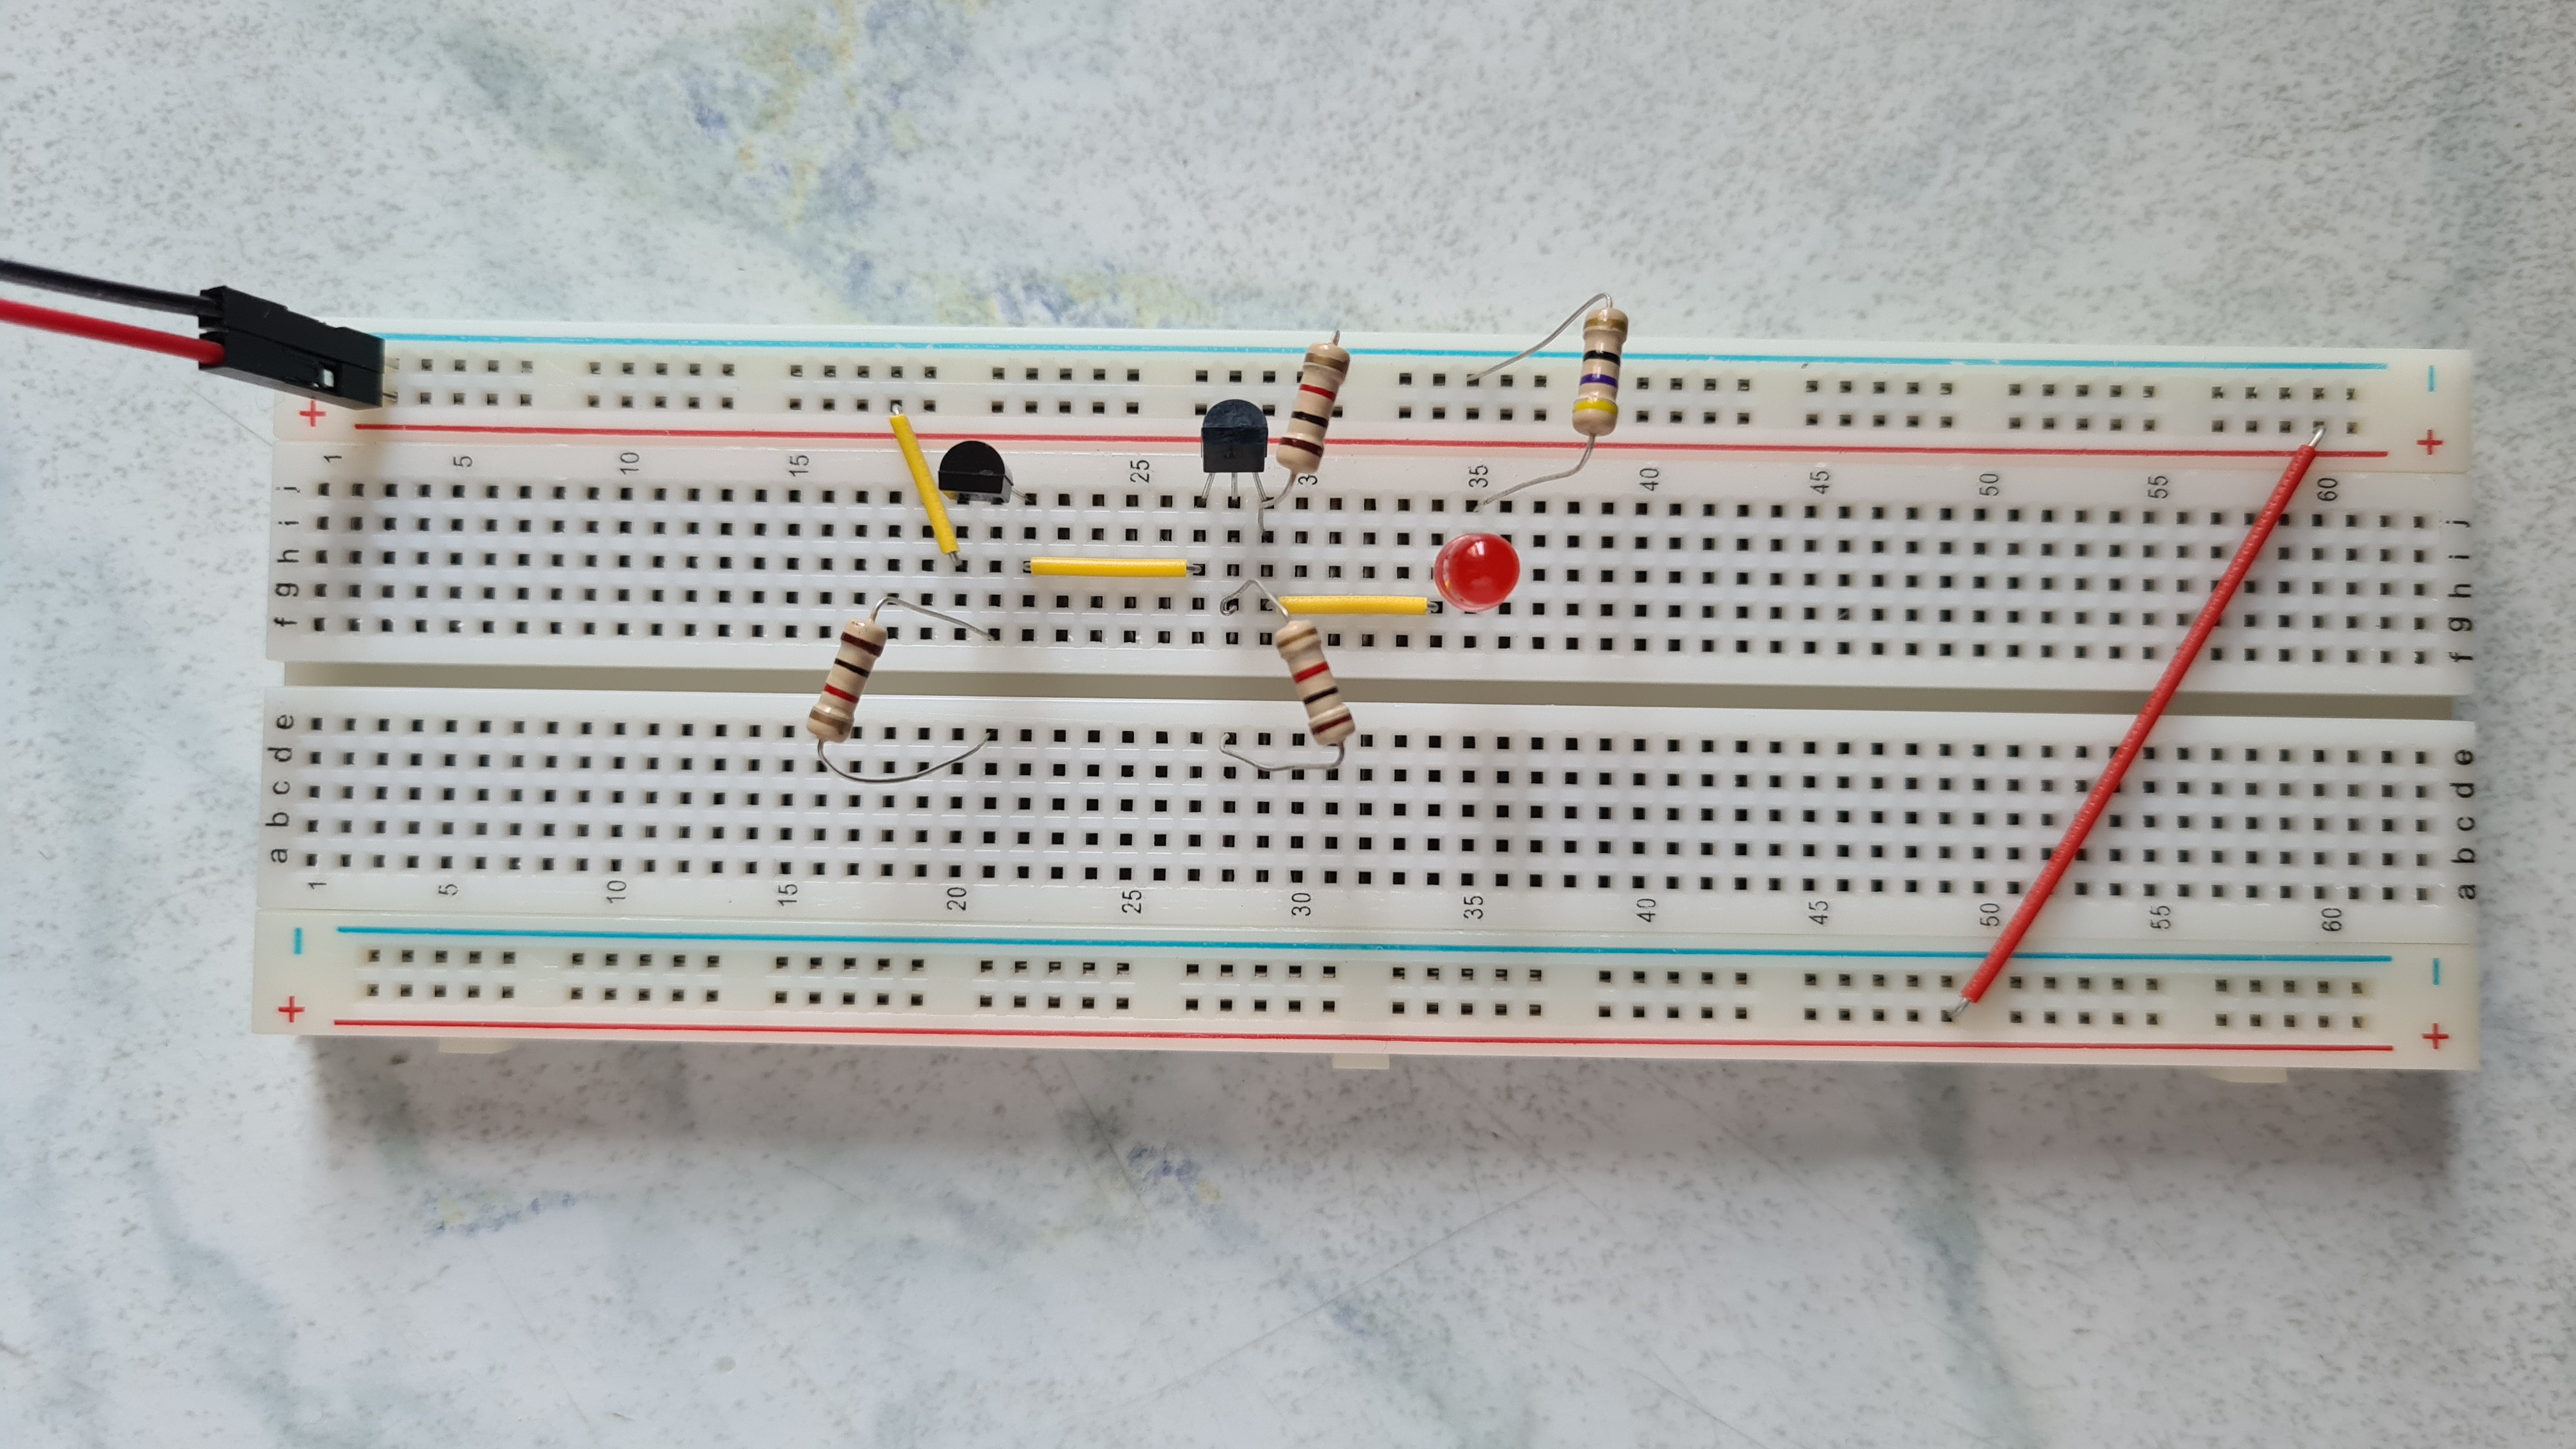
\includegraphics[height=4cm, keepaspectratio]{./Fotos/UND-00.jpg}
		\vspace{1cm}
	\end{minipage}%
	\begin{minipage}{.5\textwidth}
		\centering
		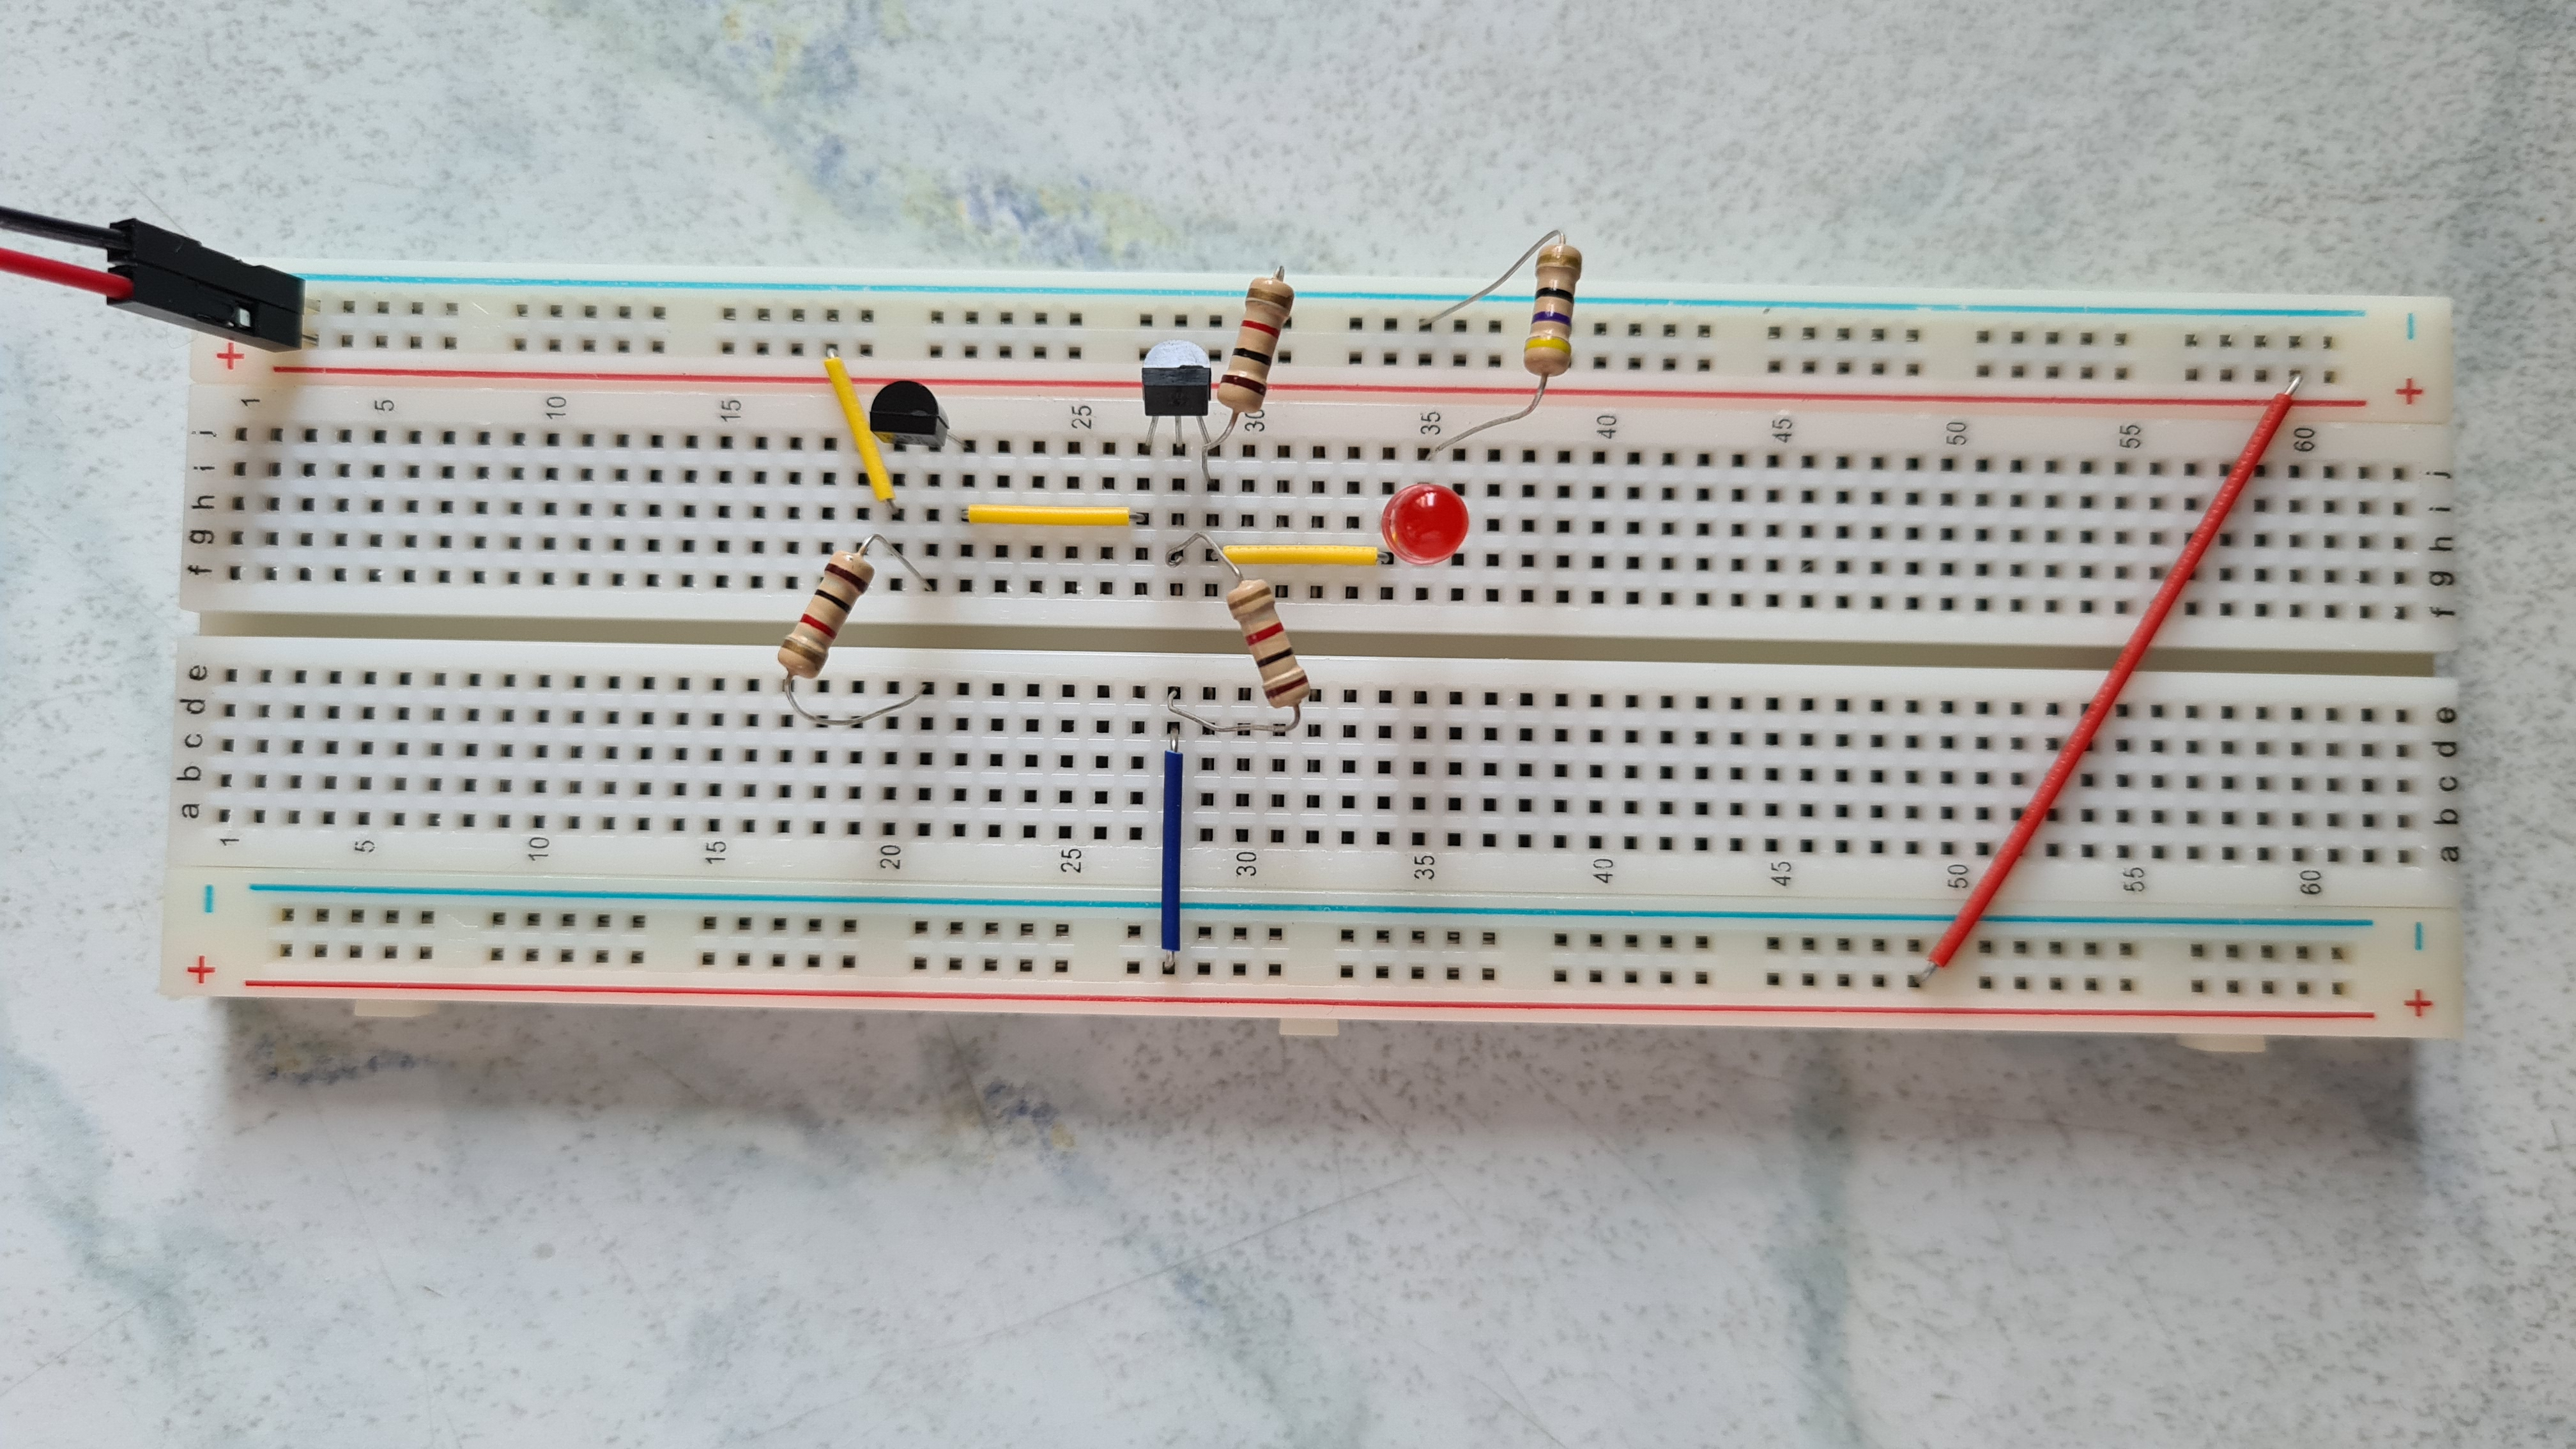
\includegraphics[height=4cm, keepaspectratio]{./Fotos/UND-01.jpg}
		\vspace{1cm}
	\end{minipage}
	\begin{minipage}{.5\textwidth}
		\centering
		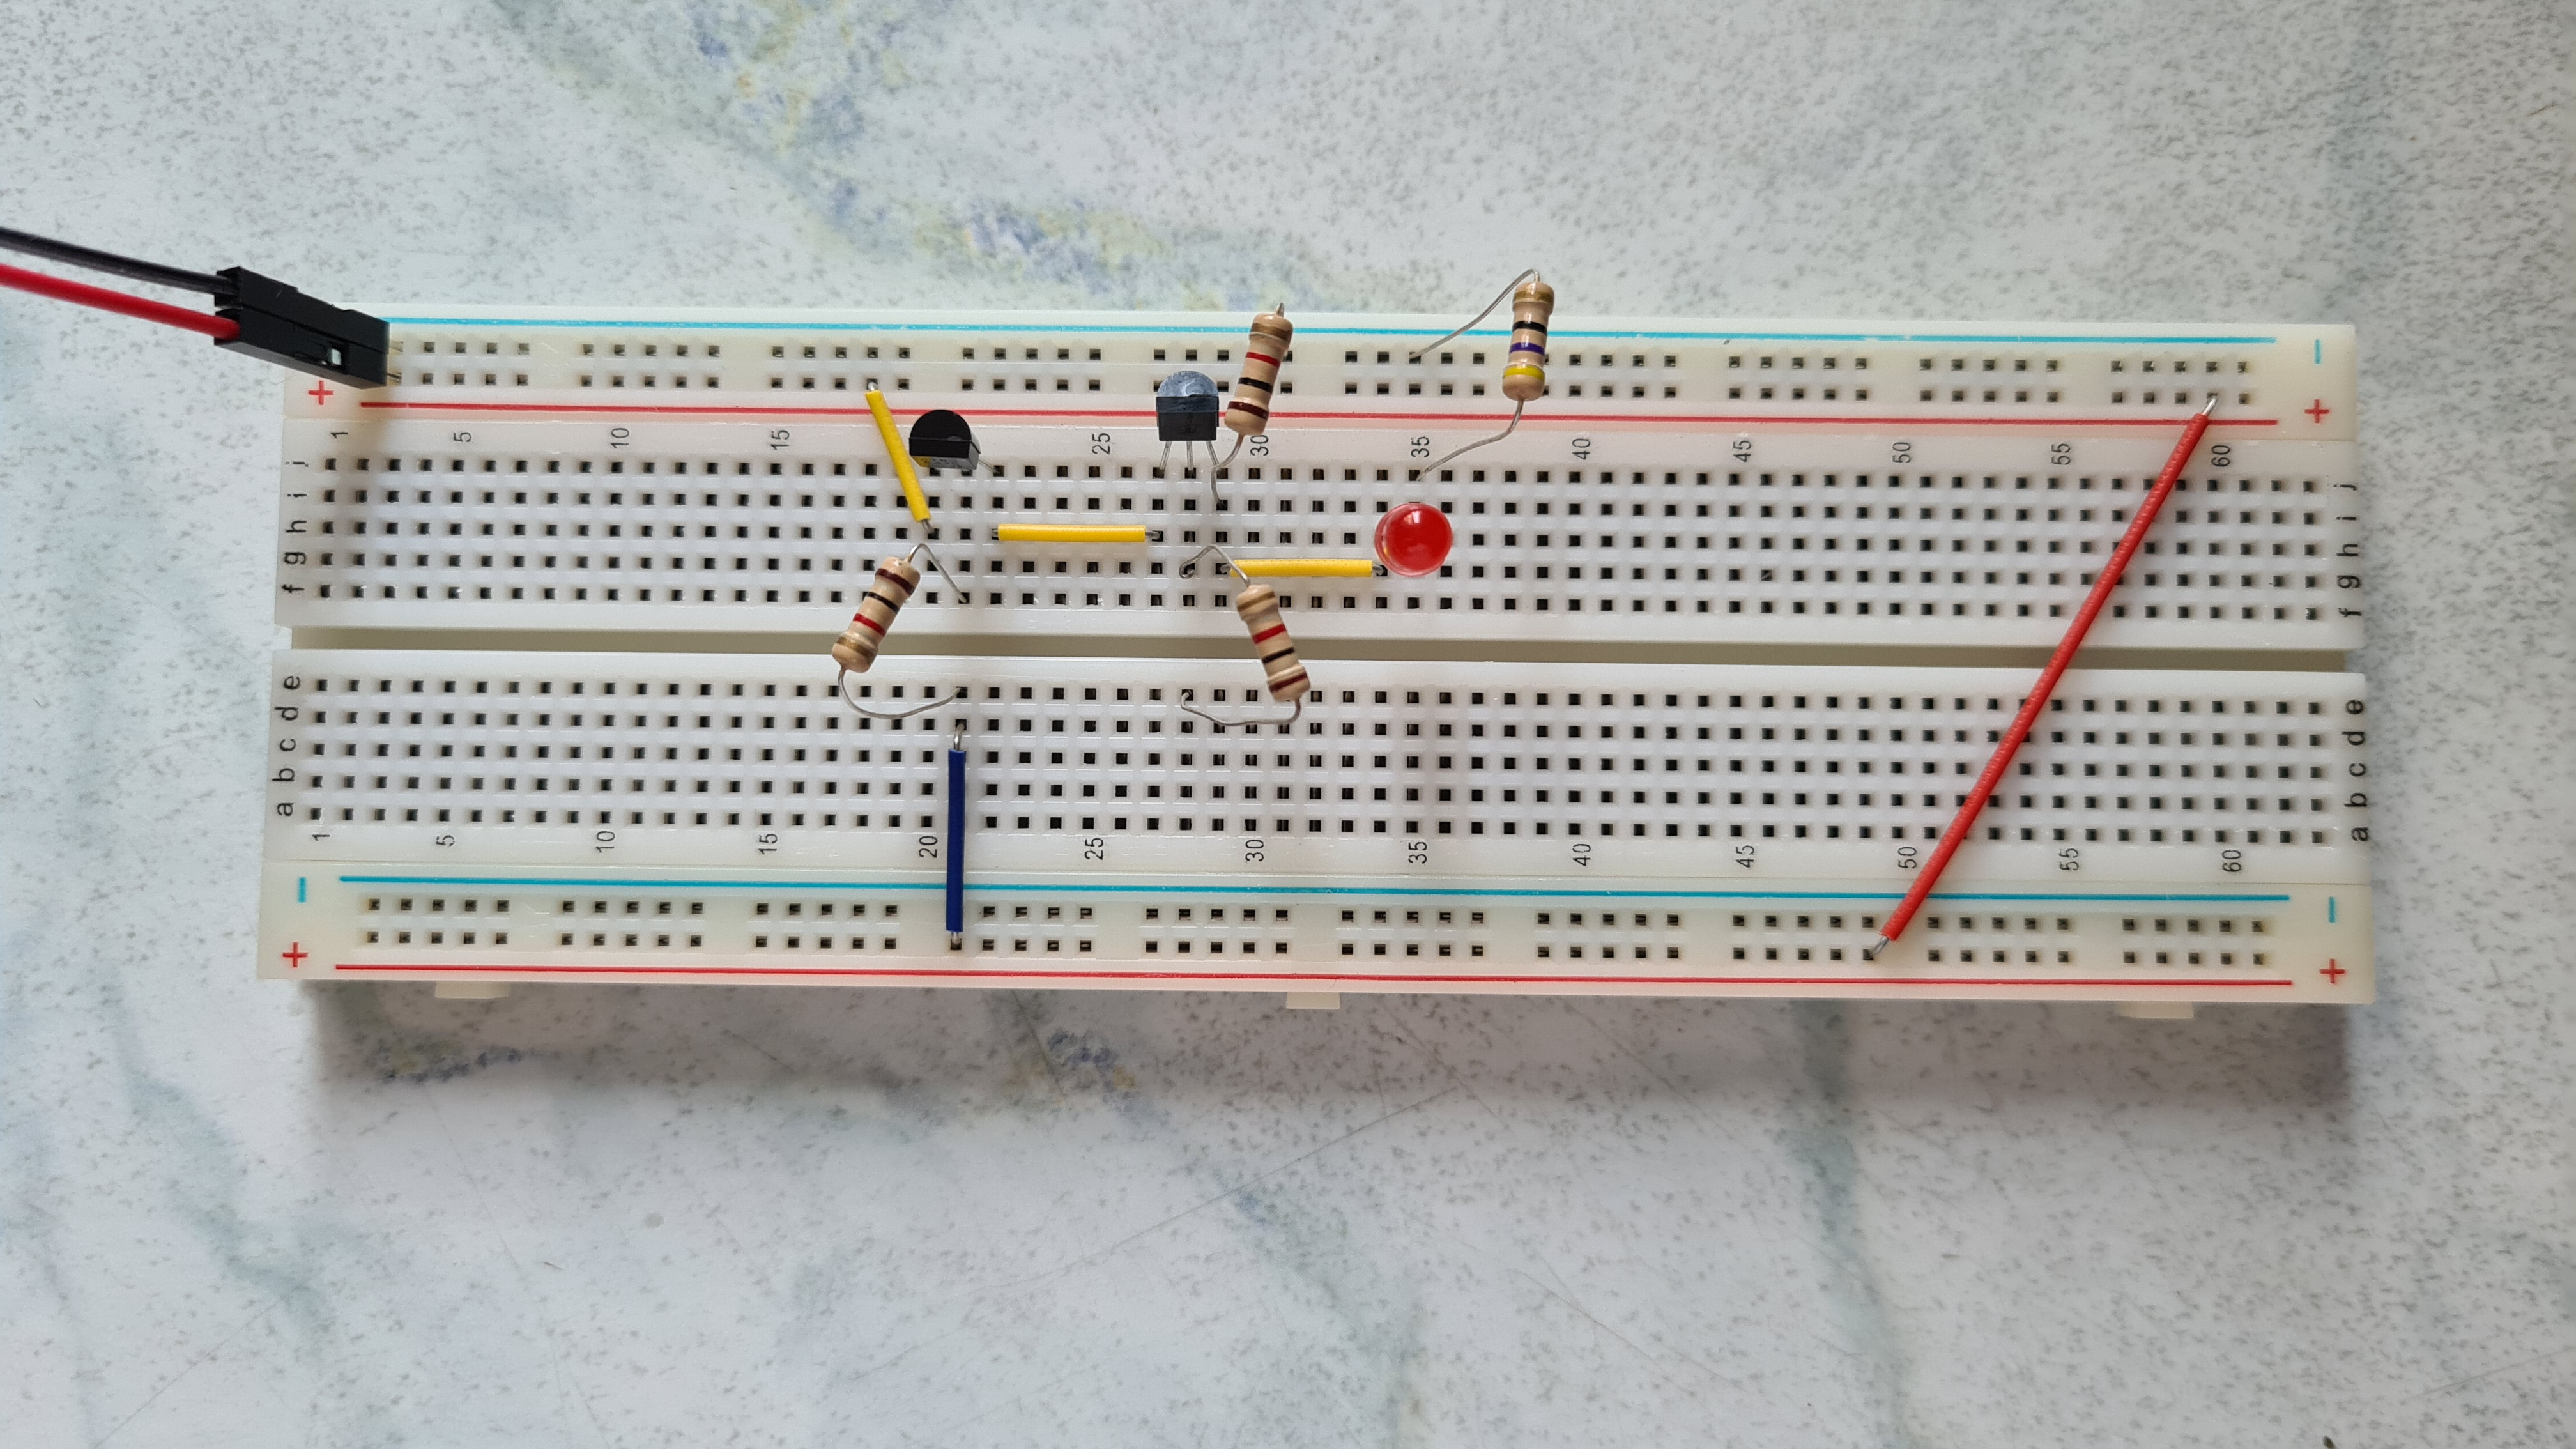
\includegraphics[height=4cm, keepaspectratio]{./Fotos/UND-10.jpg}
	\end{minipage}%
	\begin{minipage}{.5\textwidth}
		\centering
		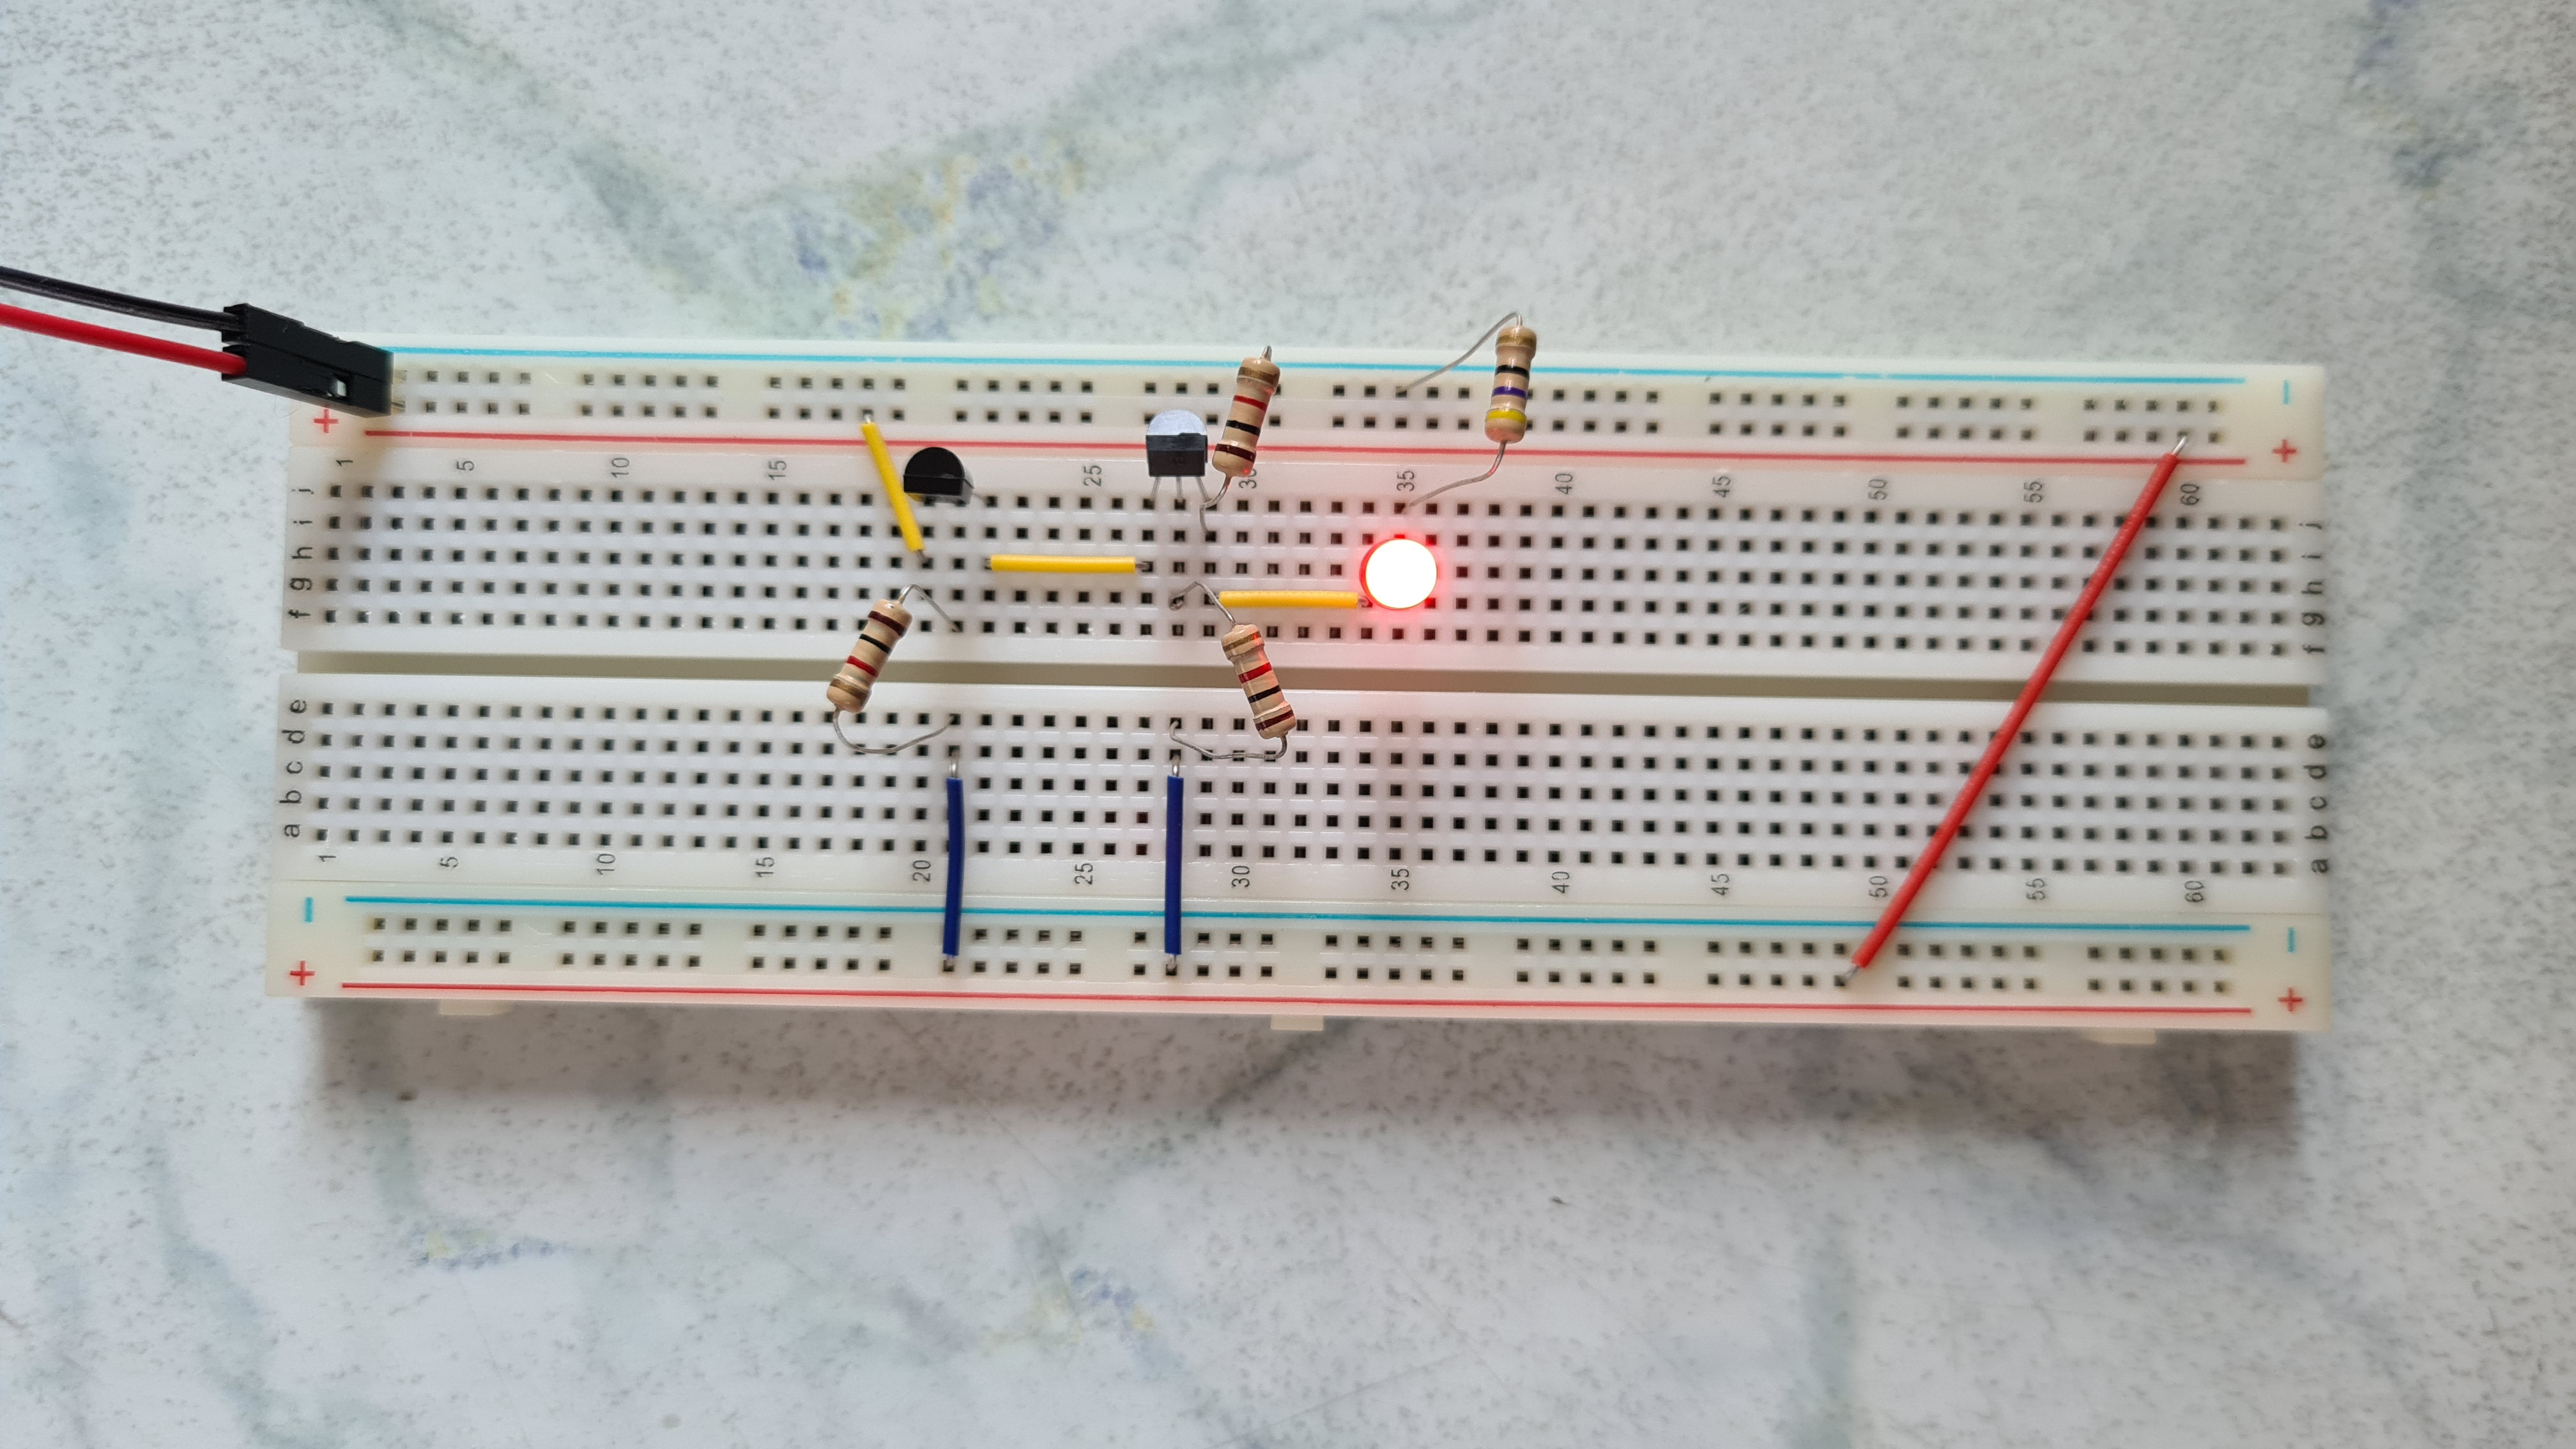
\includegraphics[height=4cm, keepaspectratio]{./Fotos/UND-11.jpg}
	\end{minipage}
	\caption{Praktischer Aufbau des UND-Gatters in allen möglichen Zuständen.}
\end{figure}
\newpage
Diese Abbildung zeigt das logische UND-Gatter auf einem Steckbrett. Die vier möglichen Zustände der Eingabeanschlüsse sind durch die blauen Drähte gegen \glqq{}+\grqq{} erkennbar. Im letzten Bild sind A und B durch diese Drähte mit HIGH verbunden. Die dadurch anliegende Spannung an Out ist durch die leuchtende LED zu erkennen.

\subsection{ODER-Gatter}
\begin{figure}[h]
	\centering
	\hspace{1cm}
	\begin{tabular}{|c|c|c|}
		\hline
		\textbf{A} & \textbf{B} & \textbf{Out} \\
		\hline
		0 & 0 & 0 \\
		1 & 0 & 1 \\
		0 & 1 & 1 \\
		1 & 1 & 1 \\
		\hline
	\end{tabular}
	\caption{Wahrheitstabelle für das logische ODER-Gatter}
\end{figure}
Der Aufbau des ODER-Gatters ist dem des UND-Gatters ähnlich. Die Wahrheitstabelle zeigt, das hier Out auf HIGH liegt, sobald entweder A oder B auf HIGH liegen. Wie beim UND-Gatter kann hier auf zwei Transistoren zurückgegriffen werden. Diese in Reihe zu schalten ist hier allerdings nicht zielführend. Beide Kollektoren müssen mit Plus verbunden sein. Liegen beide Emitter auf Out, genügt das Durchschalten eines Transistors um Out auf HIGH zu setzen. Sind A und B auf LOW, so muss Out auf das Nullniveau gezogen werden. Hierfür wird erneut ein $100\Omega$ Widerstand verwendet.
\newpage
\begin{figure}[h!]
	\centering
	\begin{circuitikz}
		\draw (0, 0) node[npn](T1){$T_1$};
		\draw (2, -2) node[npn](T2){$T_2$};
		
		
		\draw (T1.B) to[R, l=$R_1$, a=\SI{1}{k\ohm}] ++(-2, 0) to[short, -o] ++(-.5, 0) node[left]{A};
		\draw (T2.B) to[R, l=$R_2$, a=\SI{1}{k\ohm}] ++(-4, 0) to[short, -o] ++(-.5, 0) node[left]{B};
		
		\draw (T1.C) to[short, -o] ++(0, 1) node[above]{$VCC$};
		\draw (T2.C) to[short] ++(0, 2) to[short, -*] ++(-2, 0);
		
		\draw (T1.E) to[short] ++(3, 0) to[short, -*] ++(0, -2);
		\draw (T2.E)++(1, 0) to[R, l=$R_3$, a=\SI{100}{\ohm}] ++(0, -2) to[short] ++(0, -.5) node[ground](GND){};
		
		\draw (T2.E) to[short, -o] ++(3, 0) node[right]{Out};
		
		\draw[gray, very thick, densely dashed] (-3, 3) -- (4.5, 3) -- (4.5, -6) -- (-3, -6) -- cycle;
		\draw (4.5, -6) node[above right, gray]{ODER-Gatter};
	\end{circuitikz}
	\caption{Schaltplan für die logische ODER-Schaltung mithilfe von npn-Transistoren.}
\end{figure}
Diese Abbildung beschreibt den Aufbau eines ODER-Gatters. Analog zum UND-Gatter liegen auch hier A und B jeweils an der Basis eines npn-Transistors.
\begin{figure}[h!]
	\begin{minipage}{.5\textwidth}
		\centering
		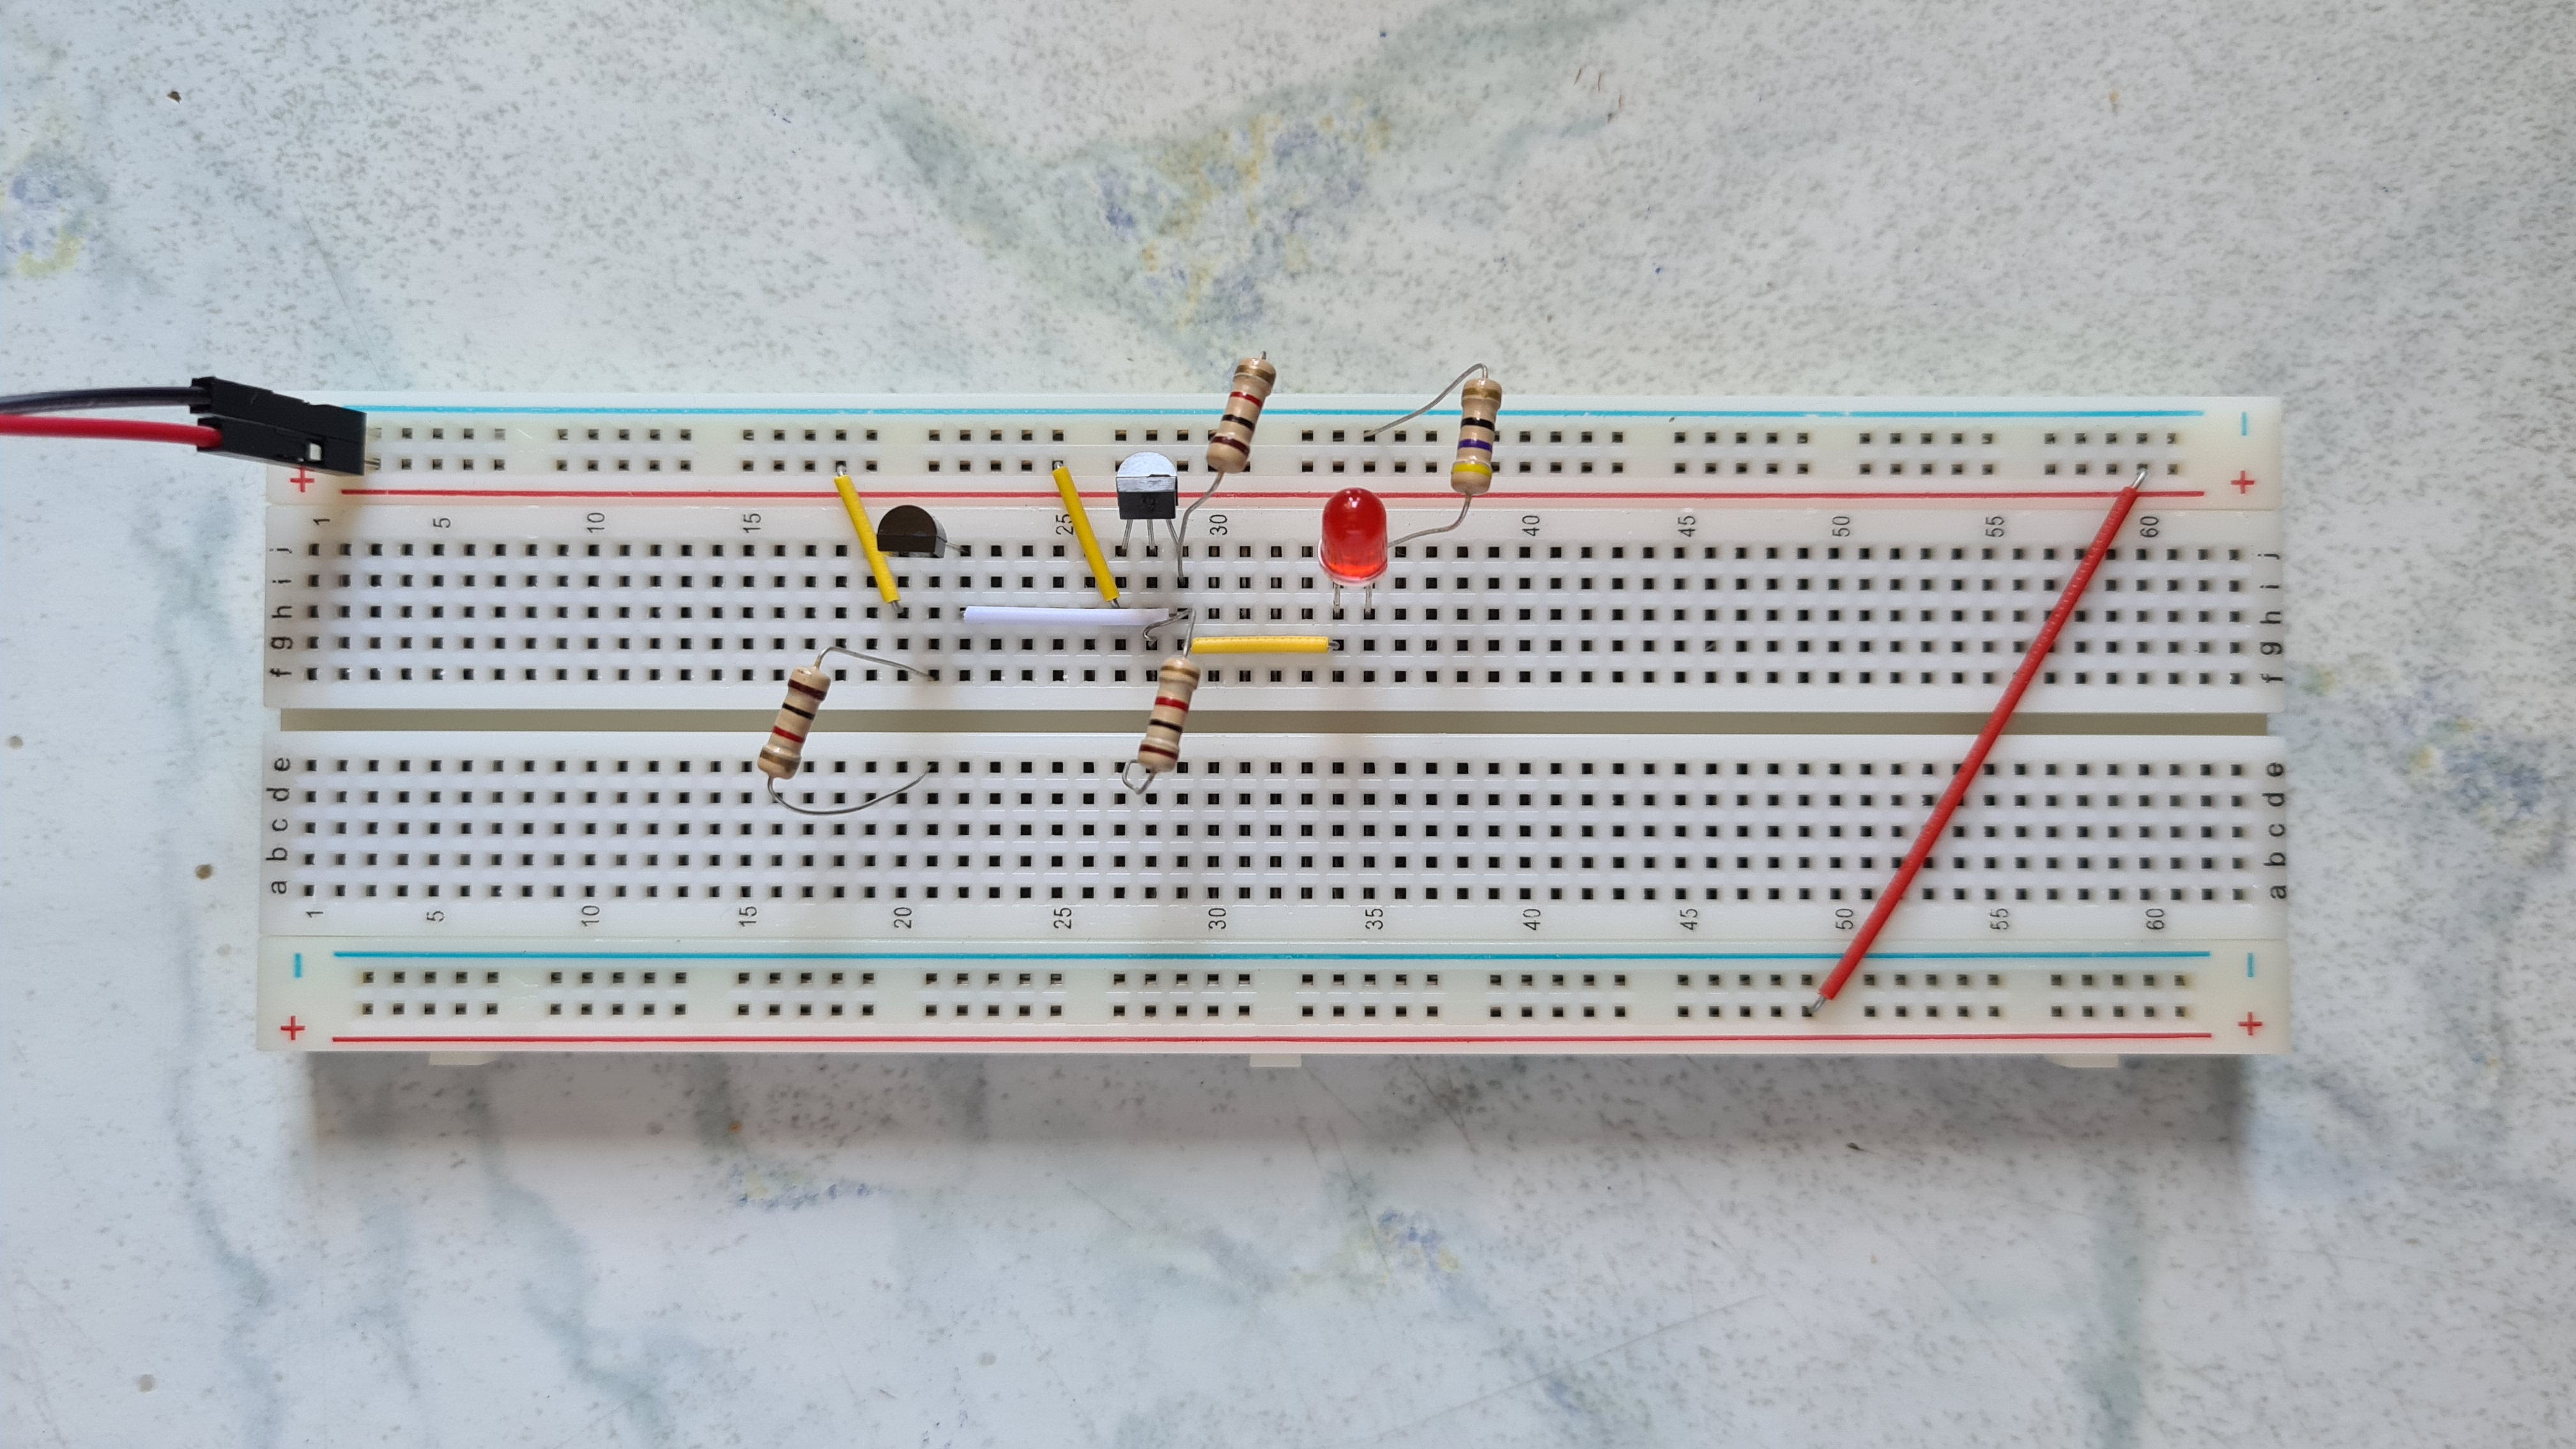
\includegraphics[height=4cm, keepaspectratio]{./Fotos/ODER-00.jpg}
		\vspace{1cm}
	\end{minipage}%
	\begin{minipage}{.5\textwidth}
		\centering
		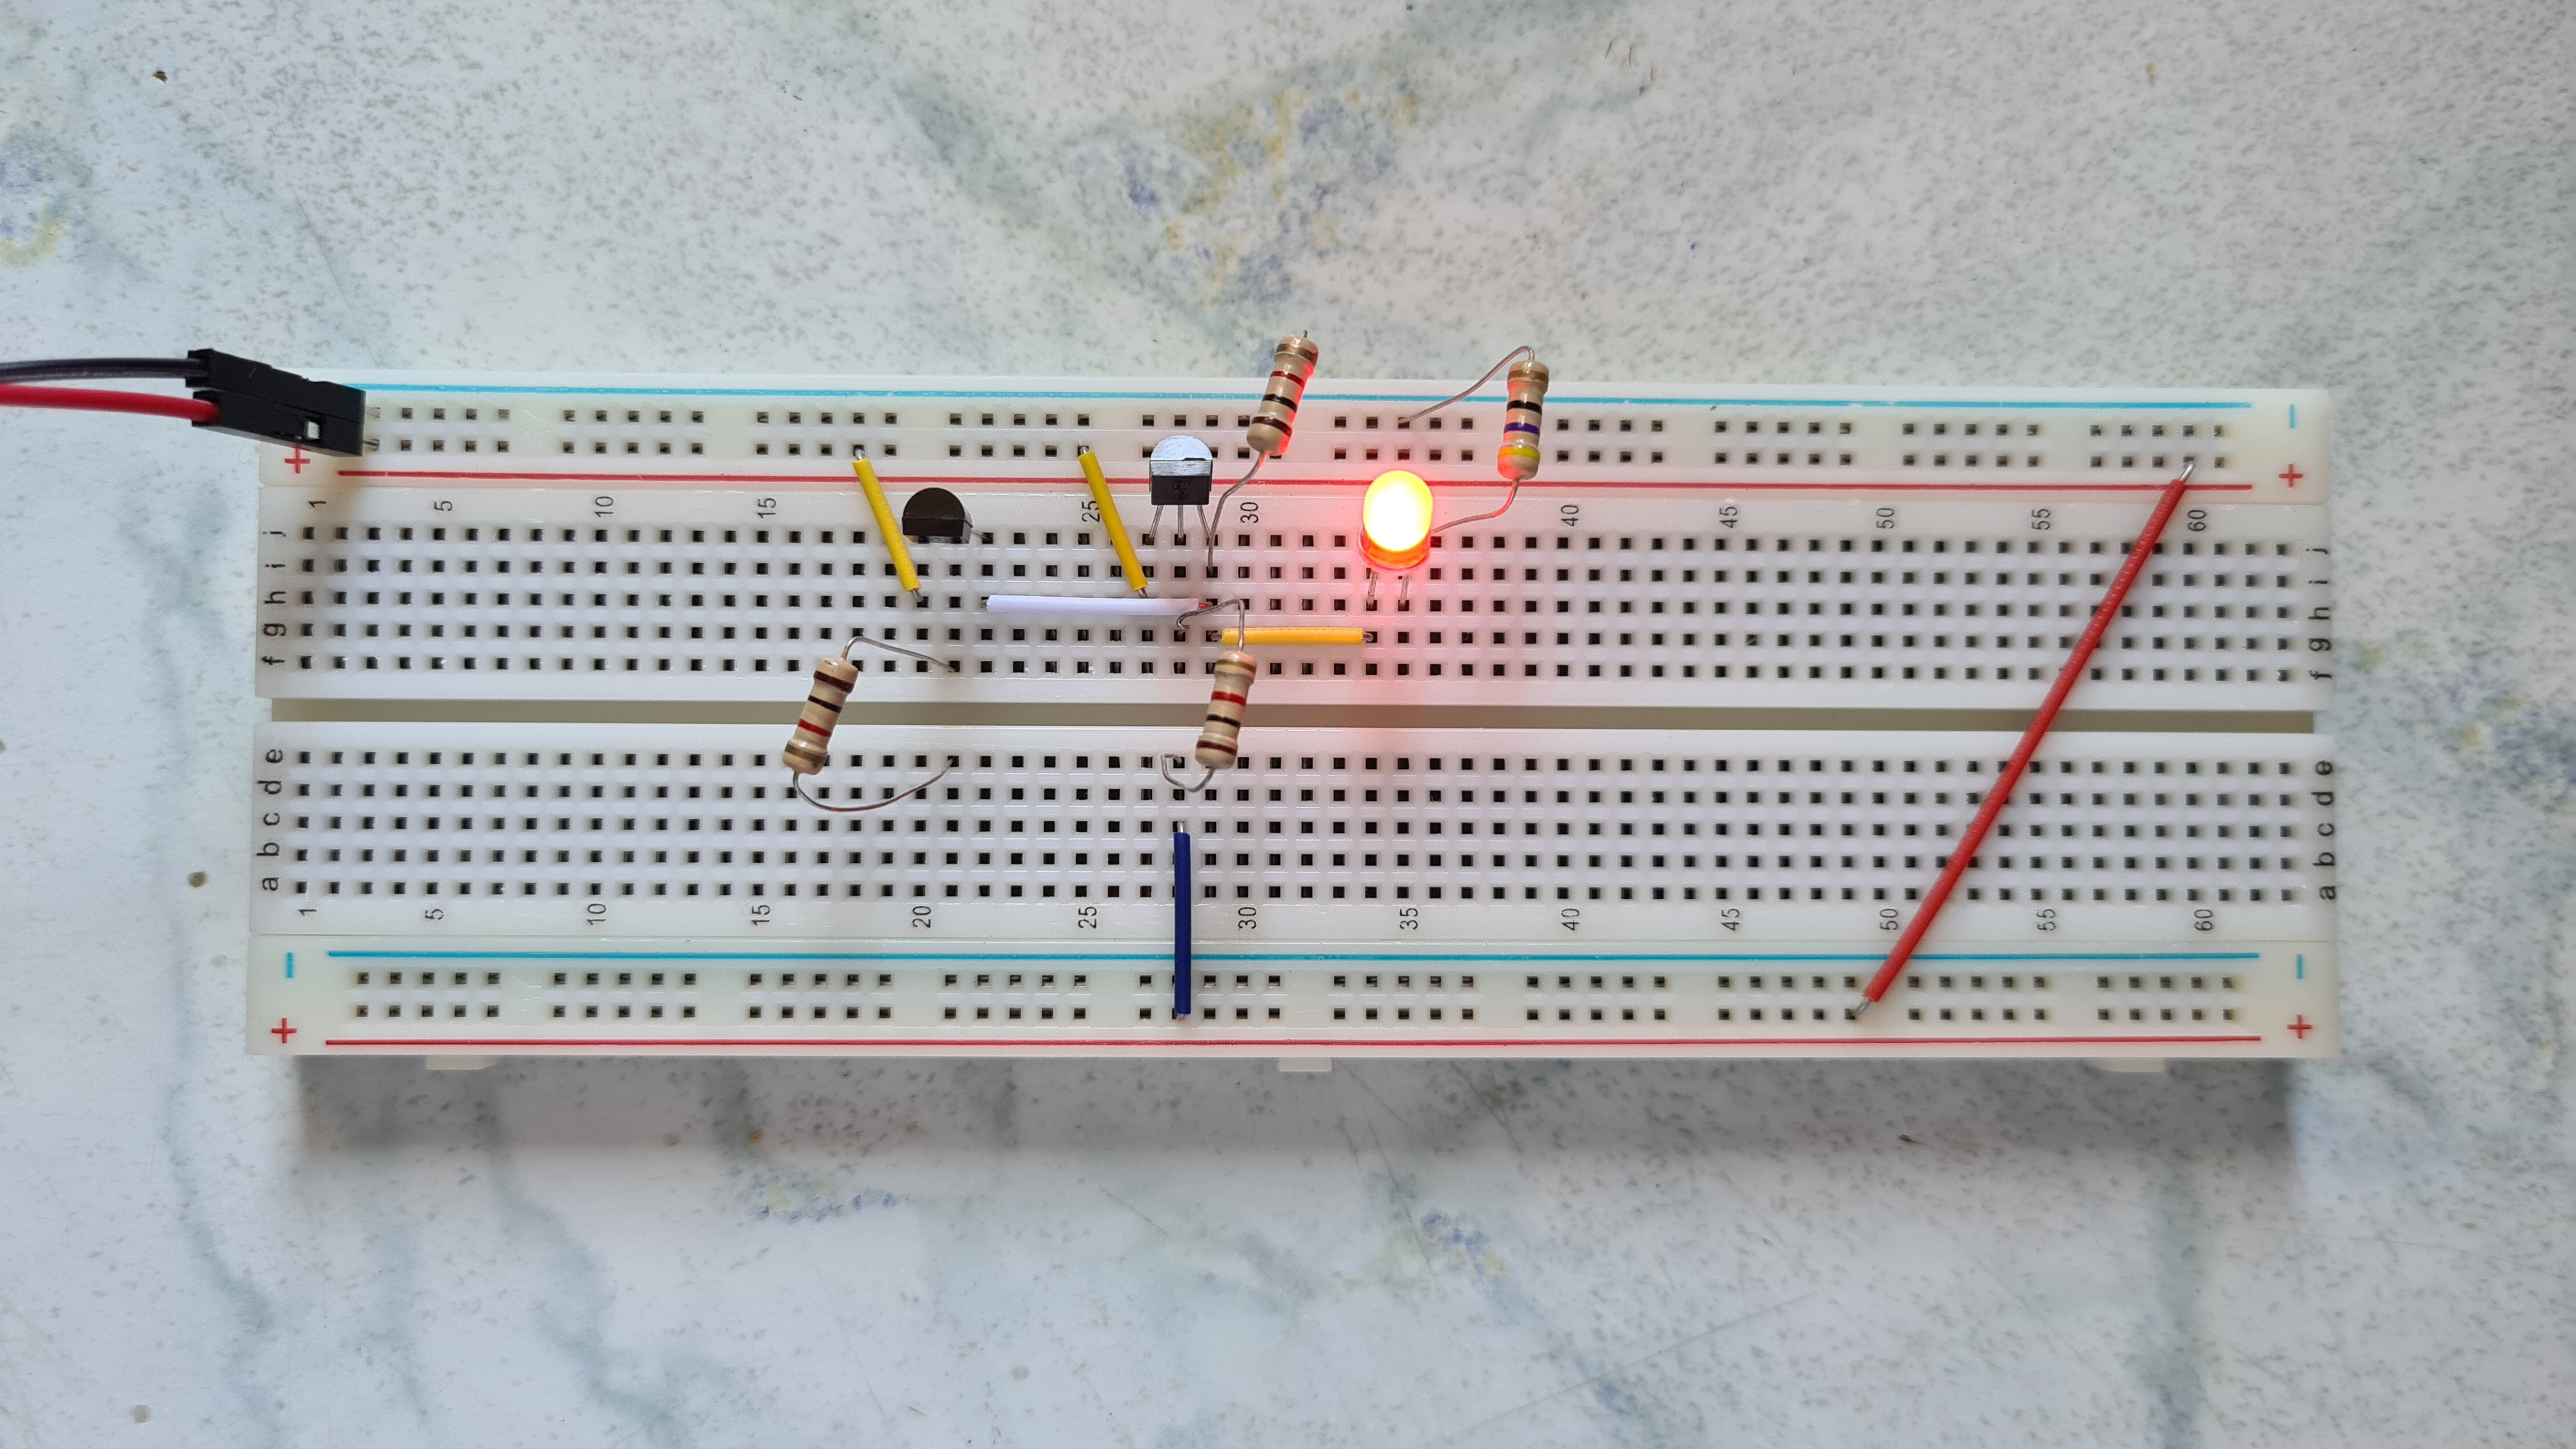
\includegraphics[height=4cm, keepaspectratio]{./Fotos/ODER-01.jpg}
		\vspace{1cm}
	\end{minipage}
	\begin{minipage}{.5\textwidth}
		\centering
		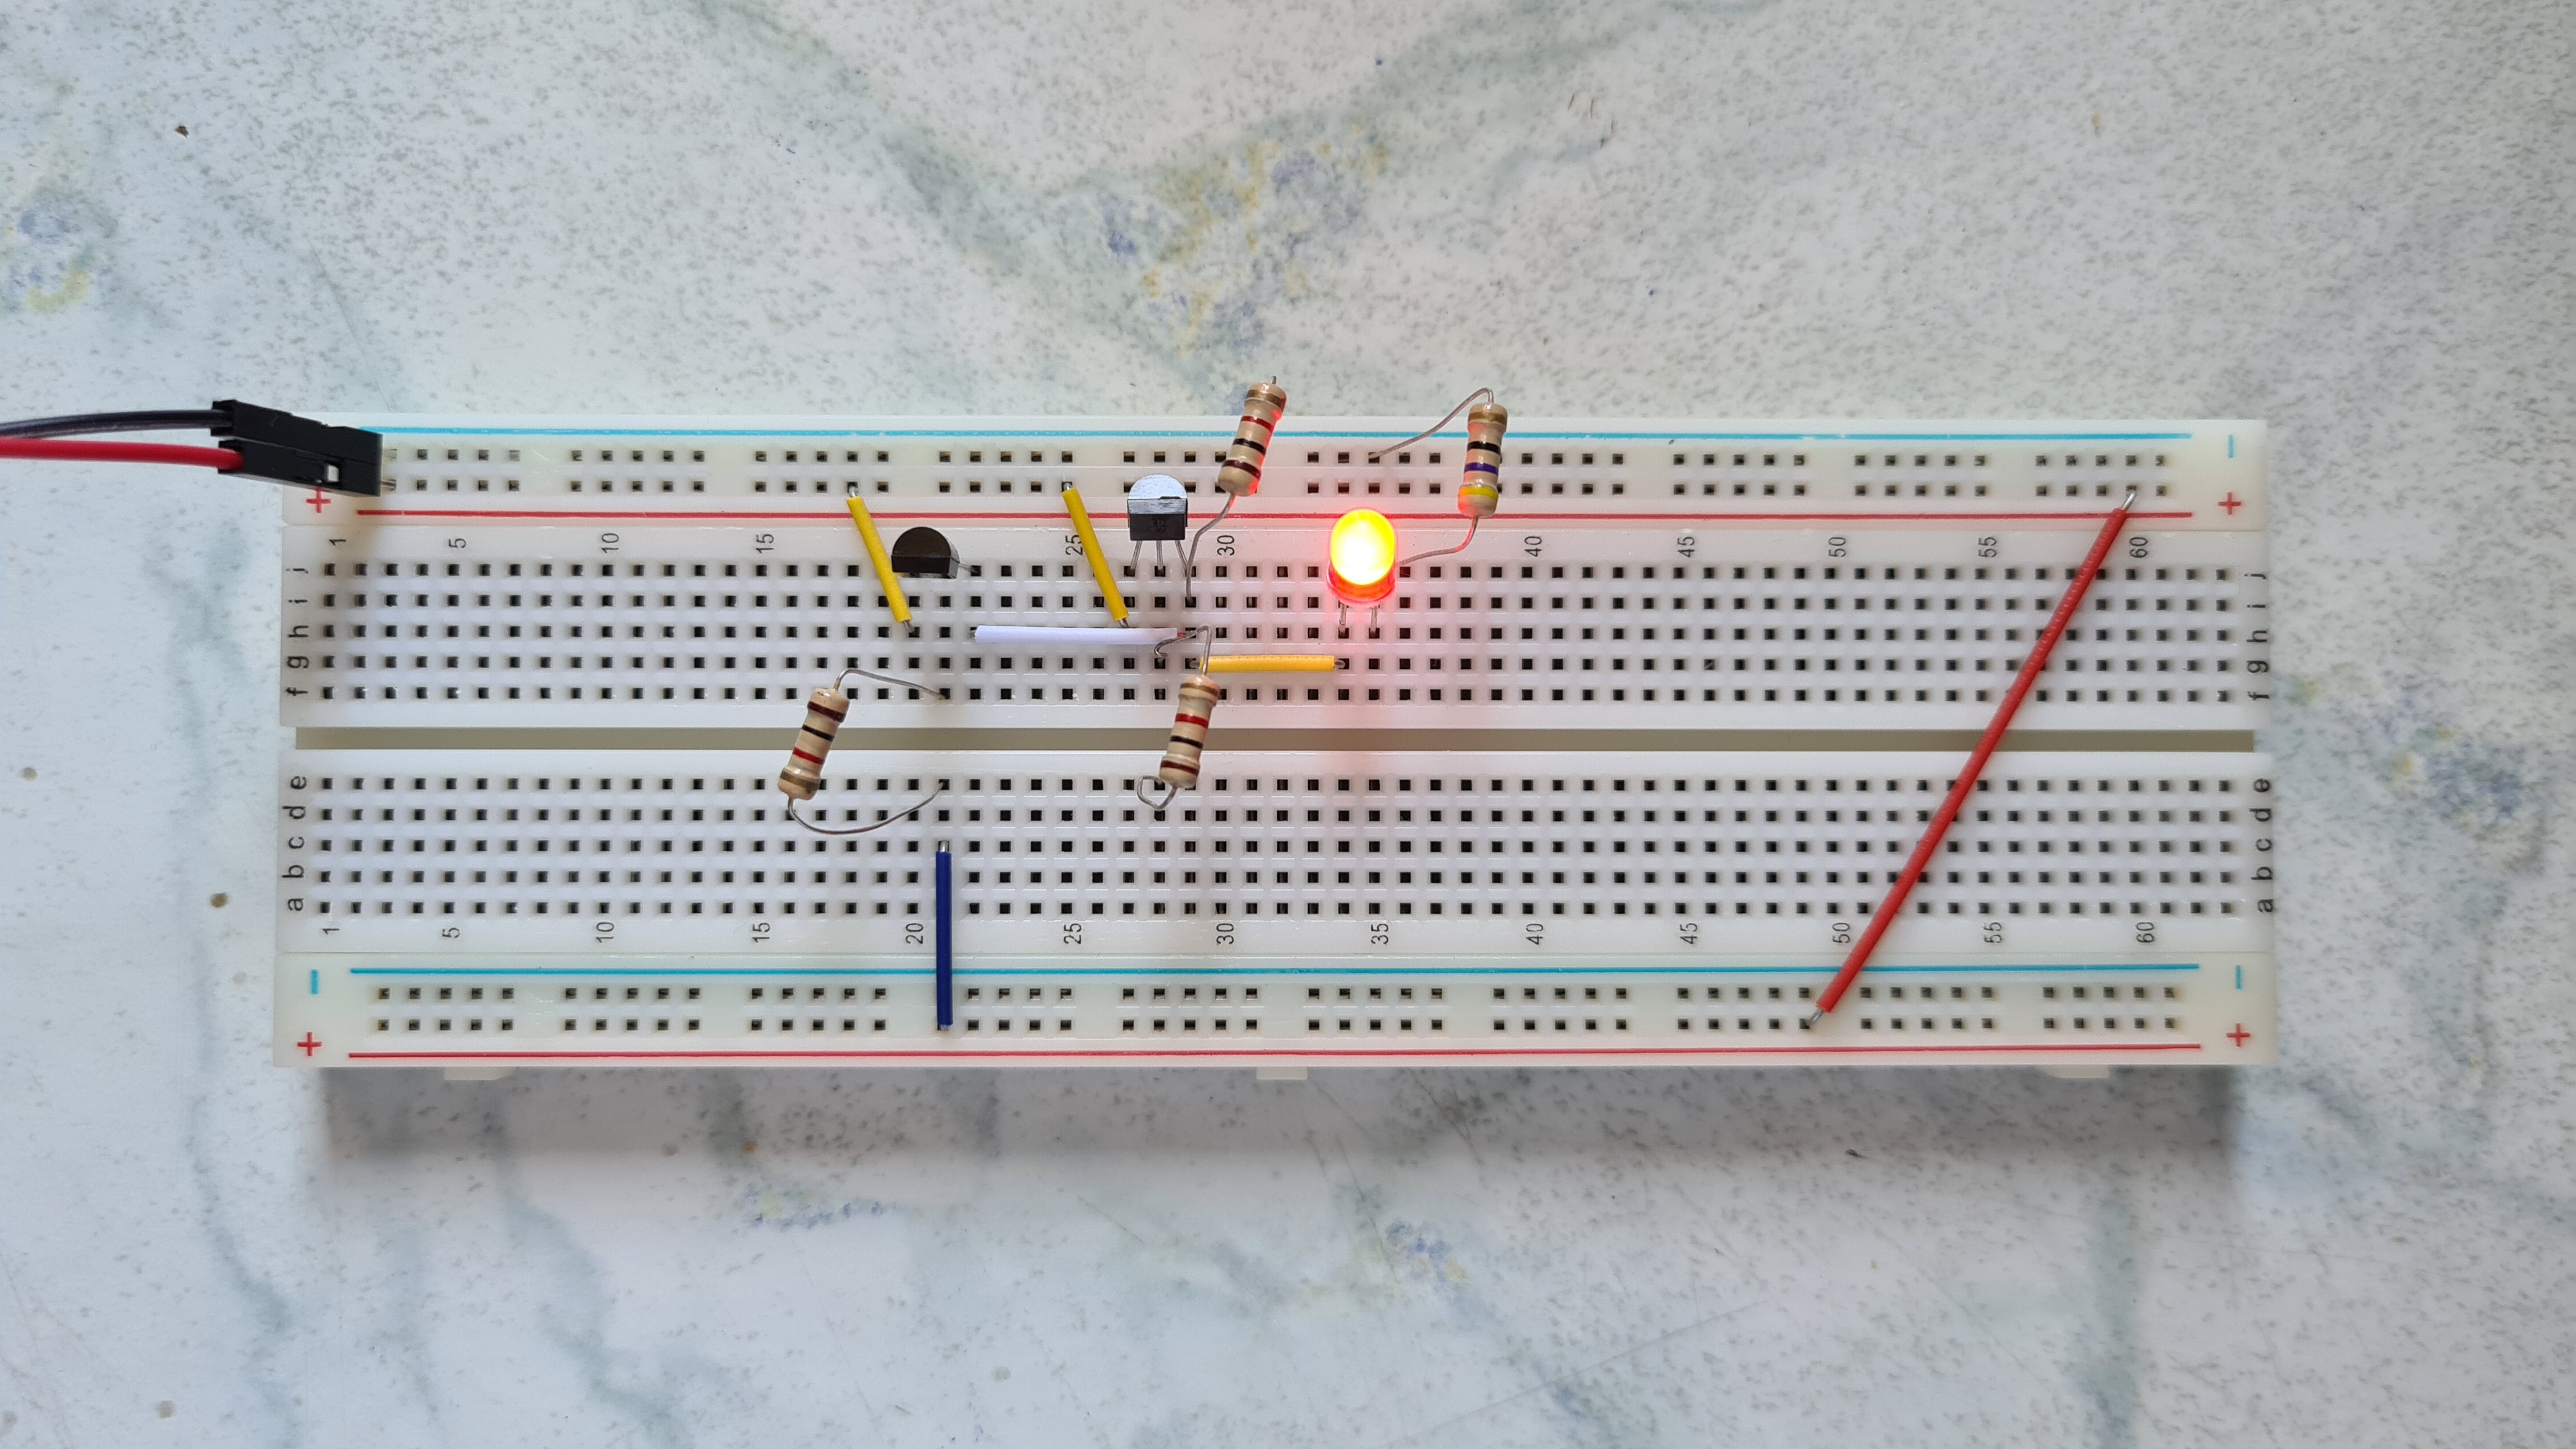
\includegraphics[height=4cm, keepaspectratio]{./Fotos/ODER-10.jpg}
	\end{minipage}%
	\begin{minipage}{.5\textwidth}
		\centering
		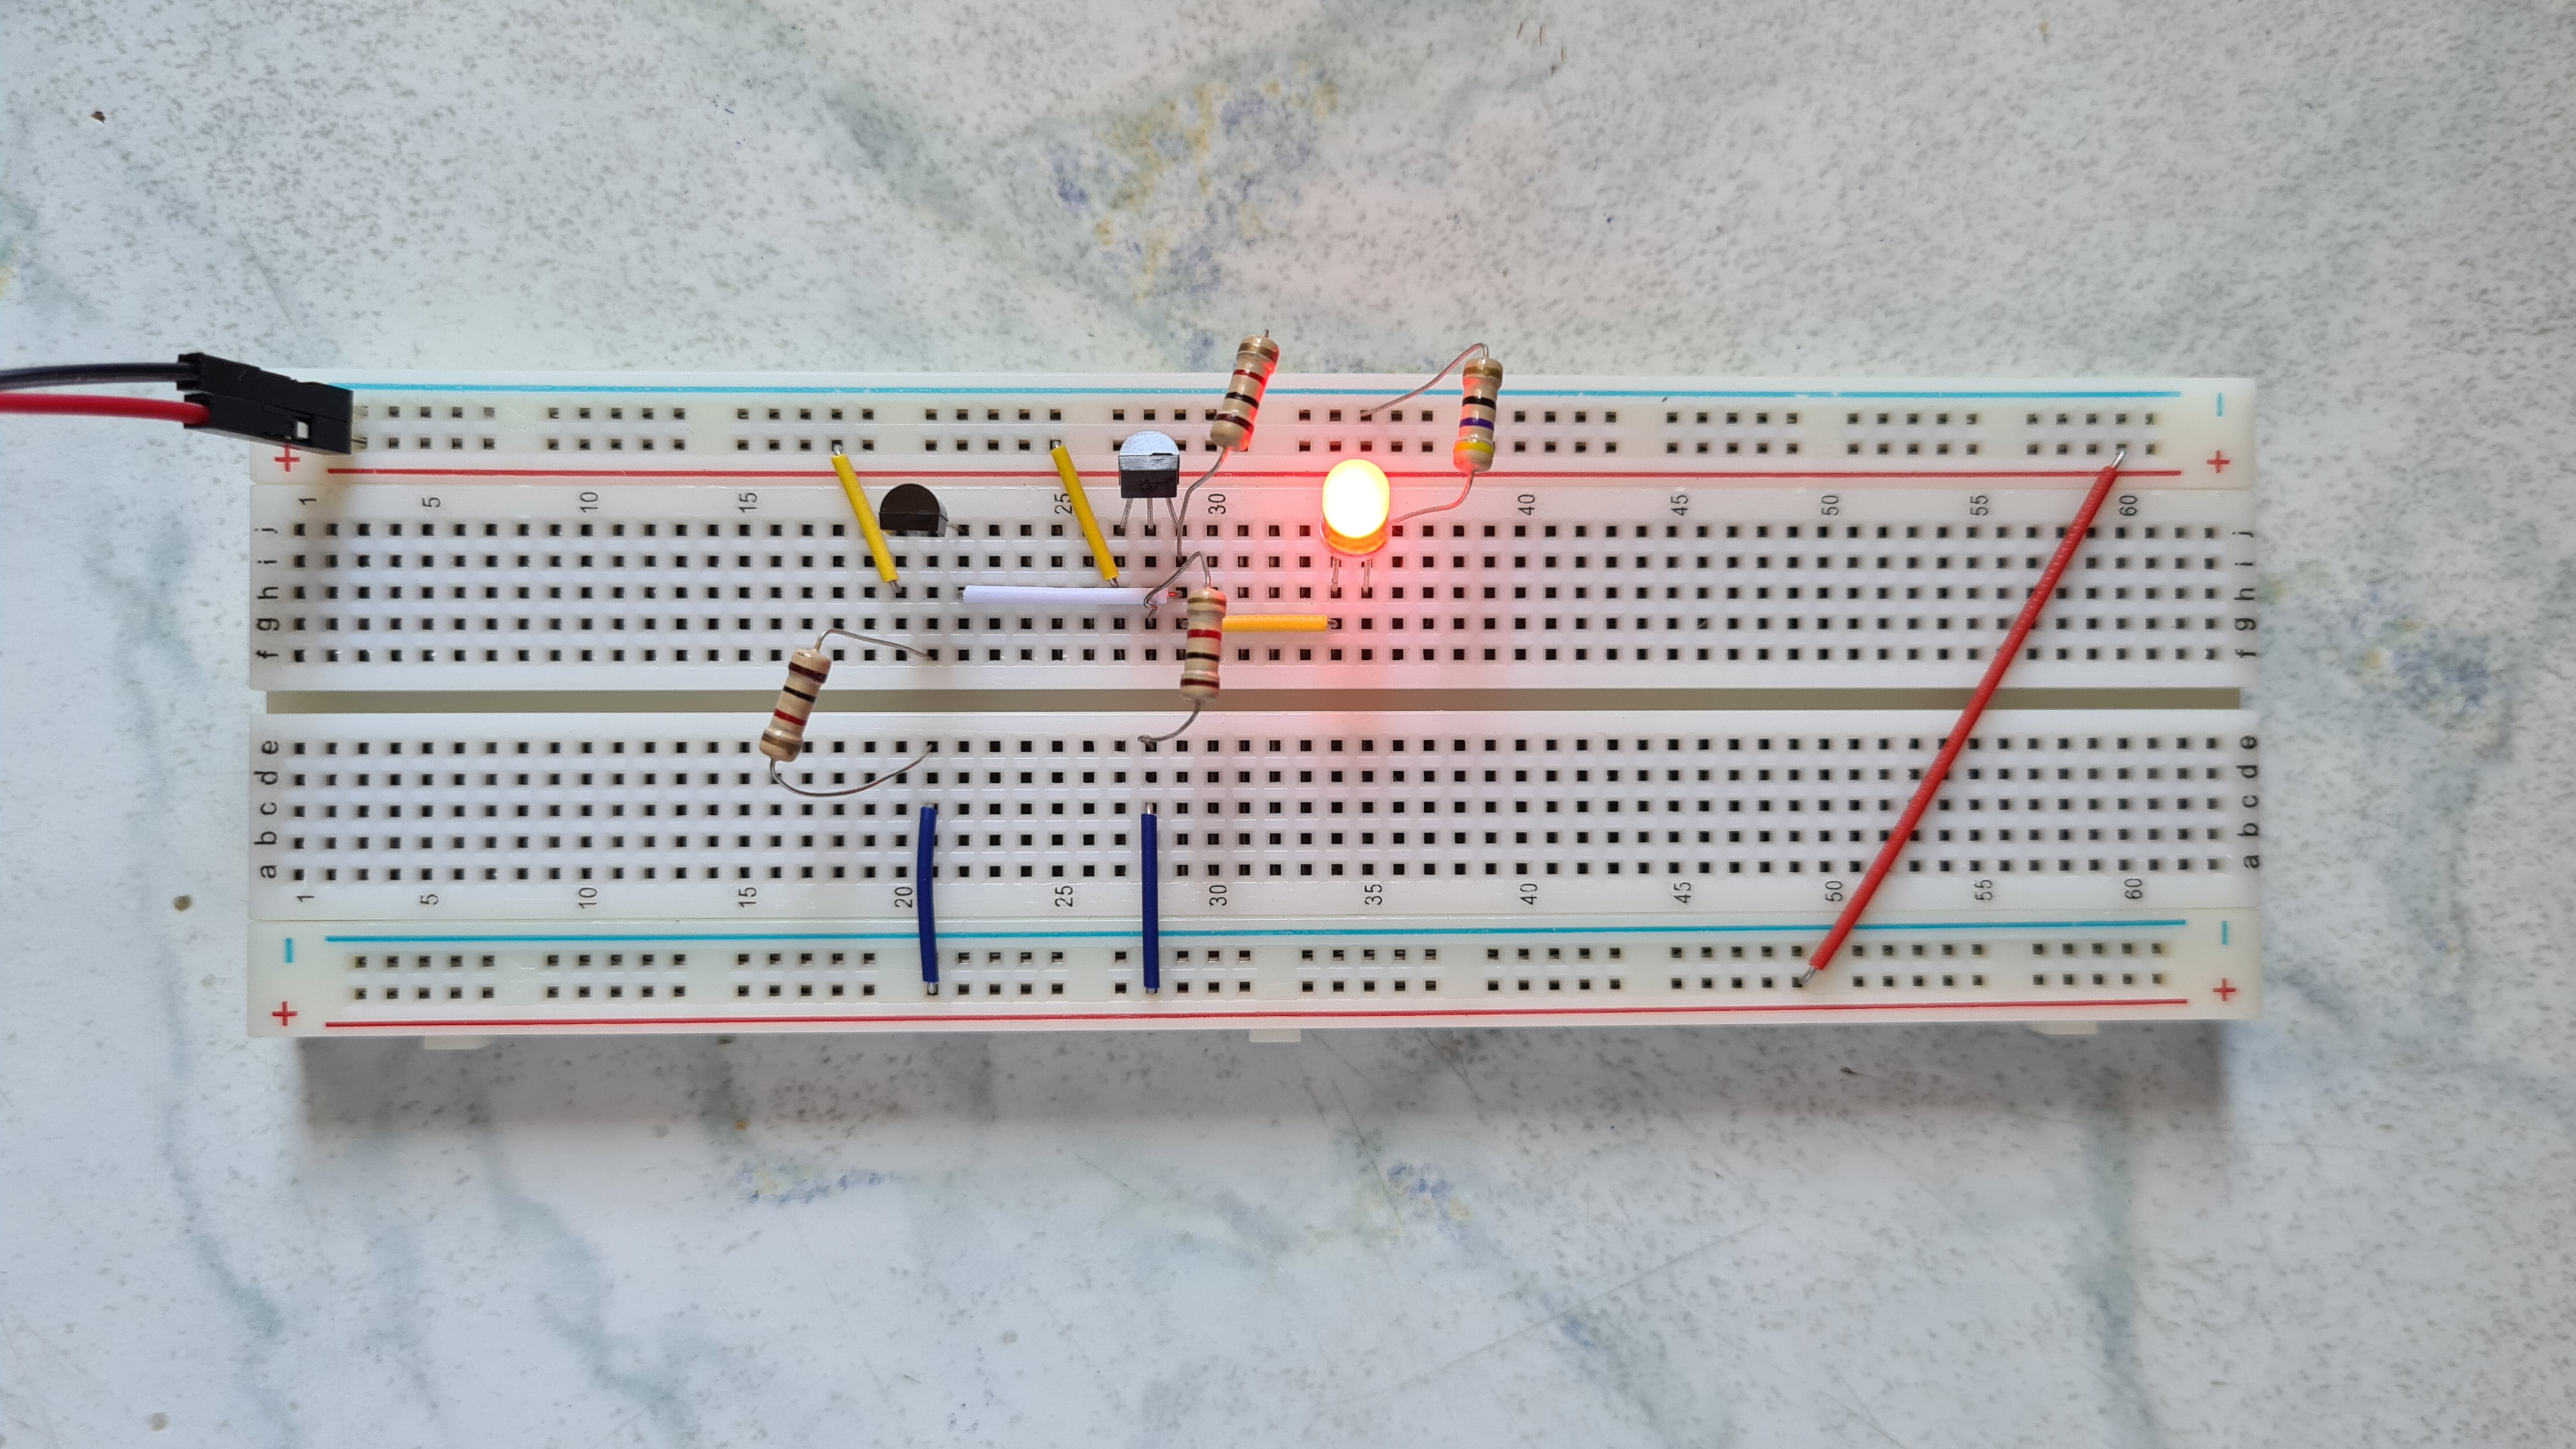
\includegraphics[height=4cm, keepaspectratio]{./Fotos/ODER-11.jpg}
	\end{minipage}
	\caption{Praktischer Aufbau des ODER-Gatters in allen möglichen Zuständen.}
\end{figure}
\newpage

\subsection{NICHT-Gatter}
\begin{figure}[h]
	\centering
	\hspace{1cm}
	\begin{tabular}{|c|c|}
		\hline
		\textbf{In} & \textbf{Out} \\
		\hline
		0 & 1 \\
		1 & 0 \\
		\hline
	\end{tabular}
	\caption{Wahrheitstabelle für das logische NICHT-Gatter}
\end{figure}
Das NICHT-Gatter besitzt lediglich einen Eingabeanschluss. Daher kann dieser auch als \glqq{}In\grqq{} bezeichnet werden. Out zeigt hier den gegenteiligen Zustand von In. So liegt Out beispielsweise auf HIGH, wenn In auf LOW gesetzt ist. Um dieses Verhalten zu erzielen muss Out konstant mit der Versorgungsspannung verbunden sein. Liegt In auf HIGH, so soll die Spannung an Out auf $\approx0\,V$ abfallen. In steuert also einen Transistor an, welcher beim Durchschalten Out mit dem Nullniveau verbindet. Da dies einen Kurzschluss zwischen Plus- und Minuspol ergeben würde, muss gegen Plus ein Widerstand installiert werden.
\begin{figure}[h!]
	\centering
	\begin{circuitikz}
		\draw (0, 0) node[npn](T1){$T_1$};
		
		\draw (T1.B) to[R, l=$R_1$, a=\SI{1}{k\ohm}] ++(-2, 0) to[short, -o] ++(-.5, 0) node[left]{In};
		
		\draw (T1.C) to[short] ++(0, .5) to[R, l=$R_2$, a=\SI{1}{k\ohm}, -o] ++(0, 2) node[above]{$VCC$};
		
		\draw (T1.E) to[short] (0, -1) node[ground](GND){};
		\draw (0, .75) to[short, *-o] ++(2.5, 0) node[right]{Out};
		
		\draw[gray, very thick, densely dashed] (-3, 4.5) -- (2, 4.5) -- (2, -2.5) -- (-3, -2.5) -- cycle;
		\draw (2, -2.5) node[above right, gray]{NICHT-Gatter};
	\end{circuitikz}
	\caption{Schaltplan für die logische NICHT-Schaltung mithilfe von npn-Transistoren.}
\end{figure}\\
Wie im Schaltplan zu erkennen, liegt Out durch einen $1000\,\Omega$-Widerstand auf HIGH. Wird In ebenso auf HIGH gesetzt, so wird das Nullpotenzial auch mit Out verbunden. Dadurch kann der Strom abfließen und die Spannung an Out fällt stark ab ($U_{Out}\leq0,1\,V$).
\begin{figure}[h!]
	\begin{minipage}{.5\textwidth}
		\centering
		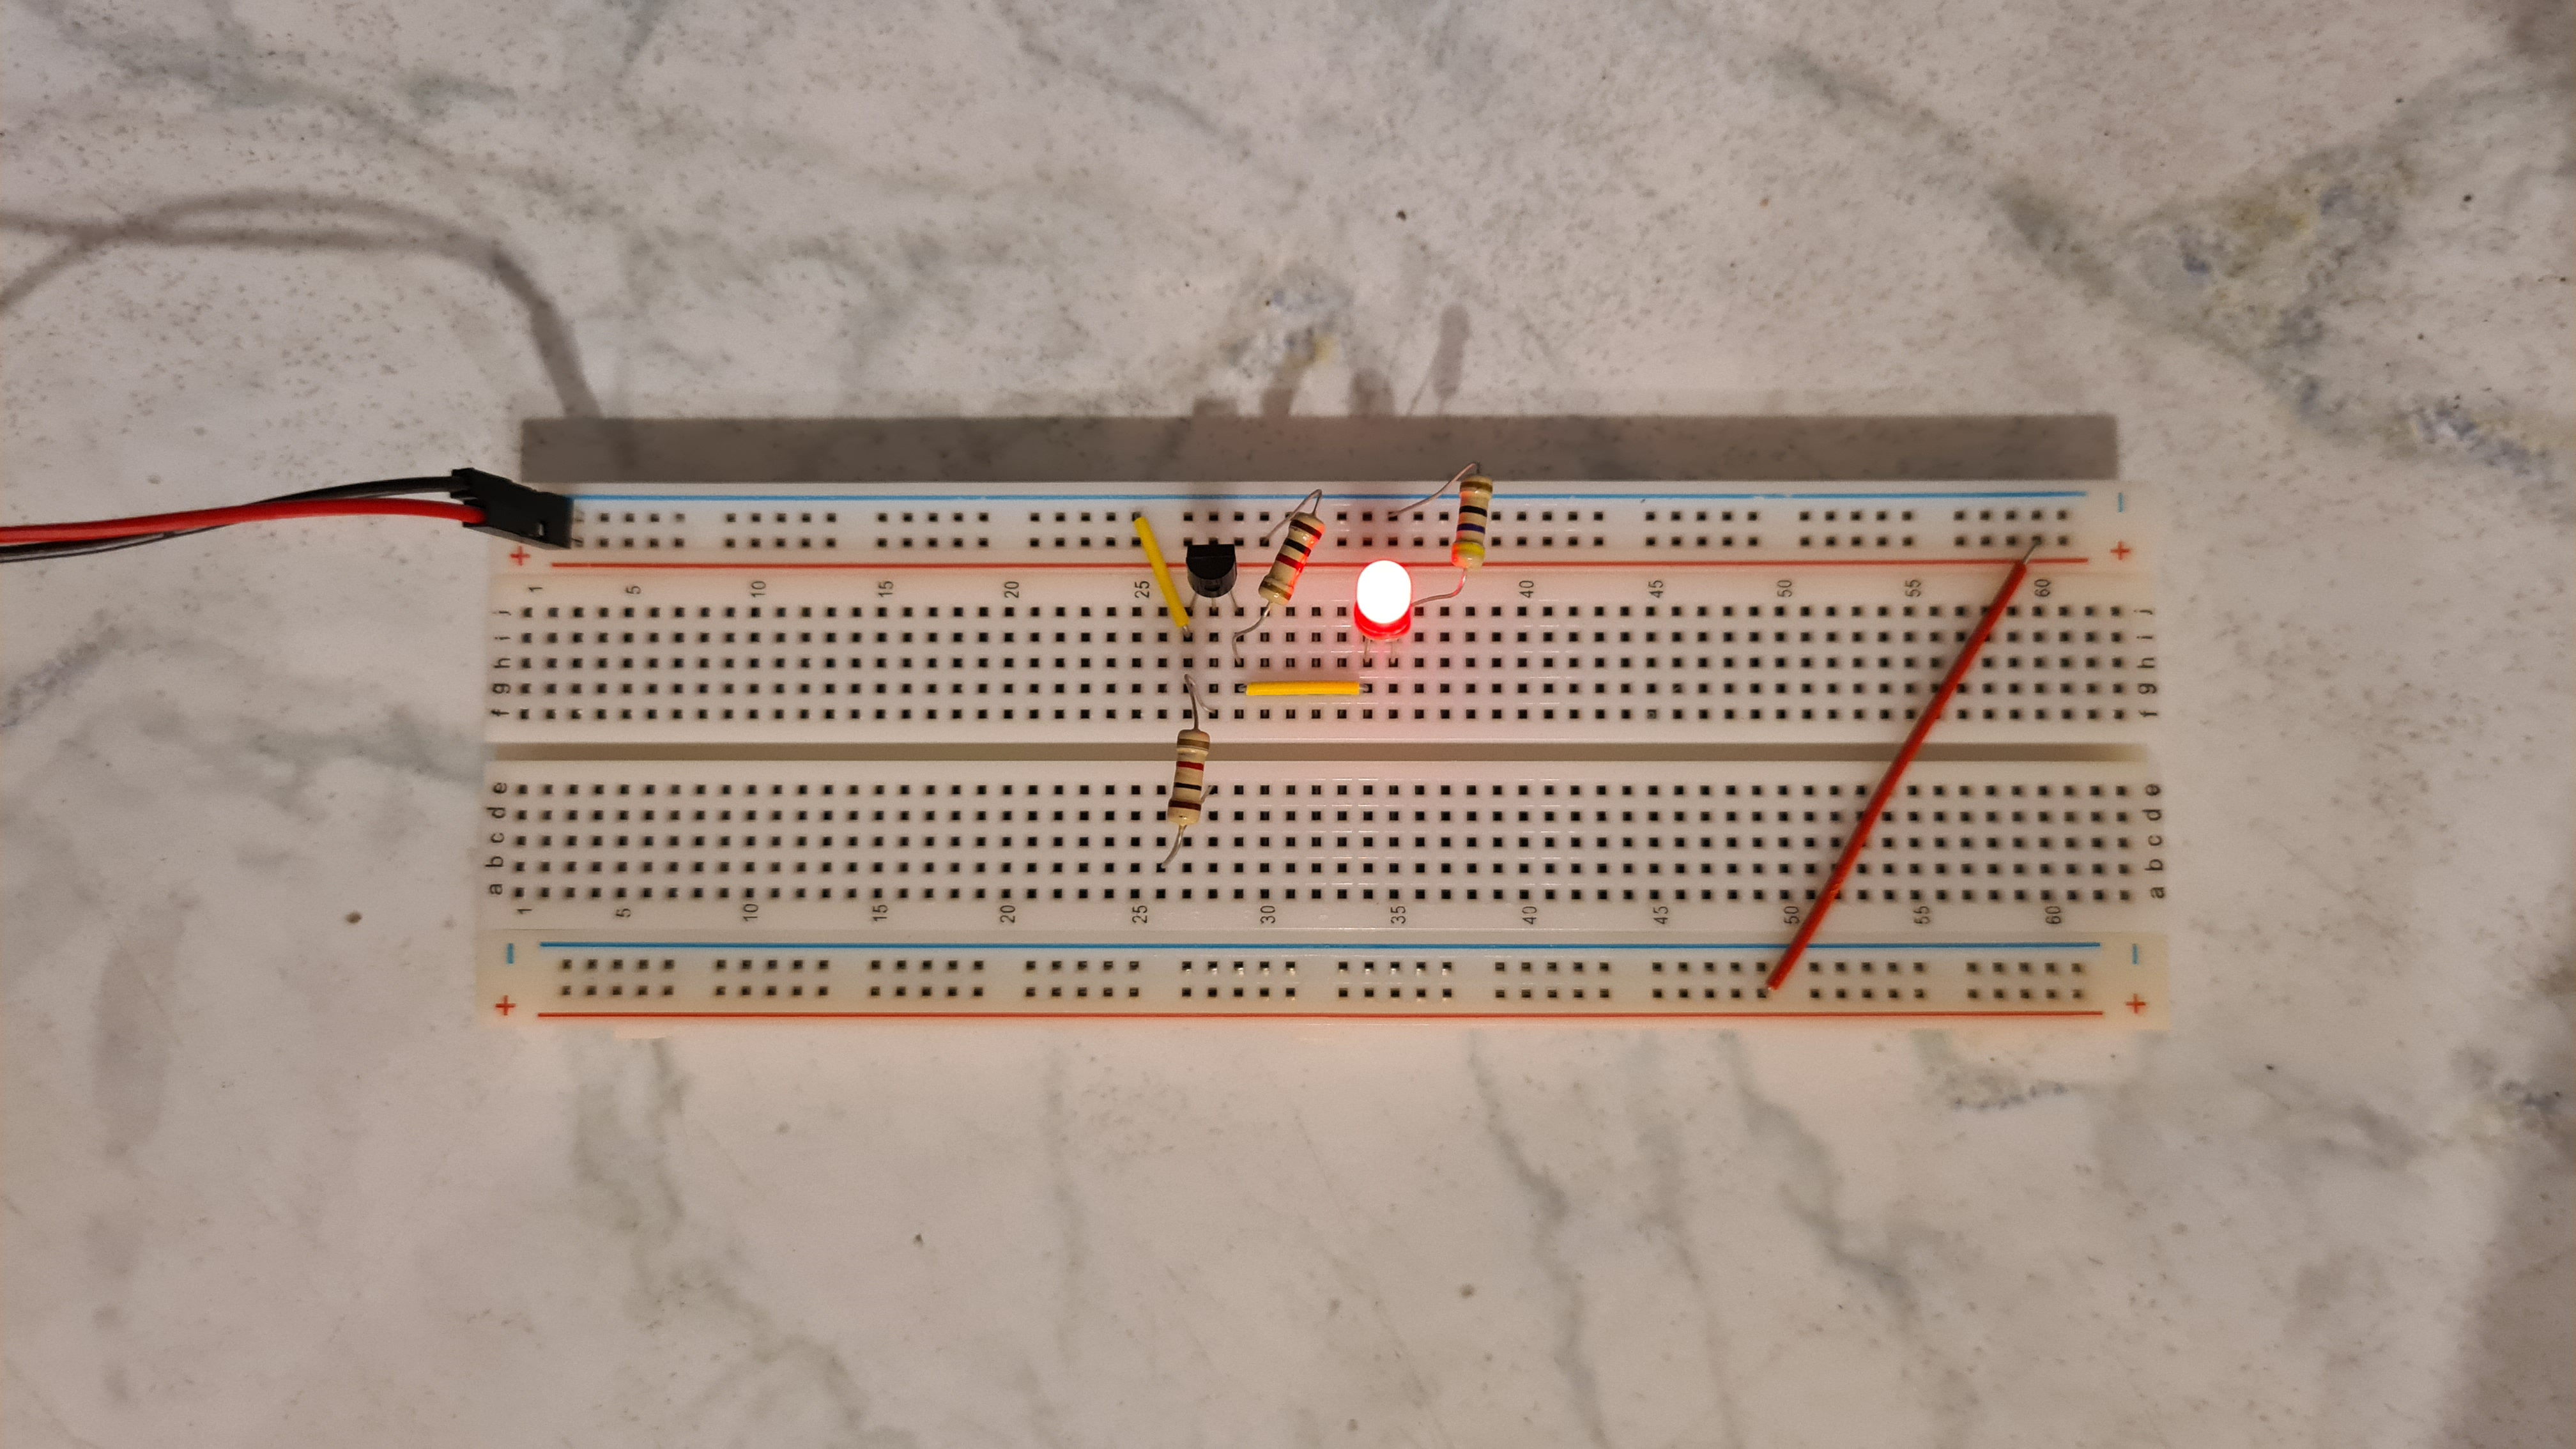
\includegraphics[height=4cm, keepaspectratio]{./Fotos/NICHT-0.jpg}
	\end{minipage}%
	\begin{minipage}{.5\textwidth}
		\centering
		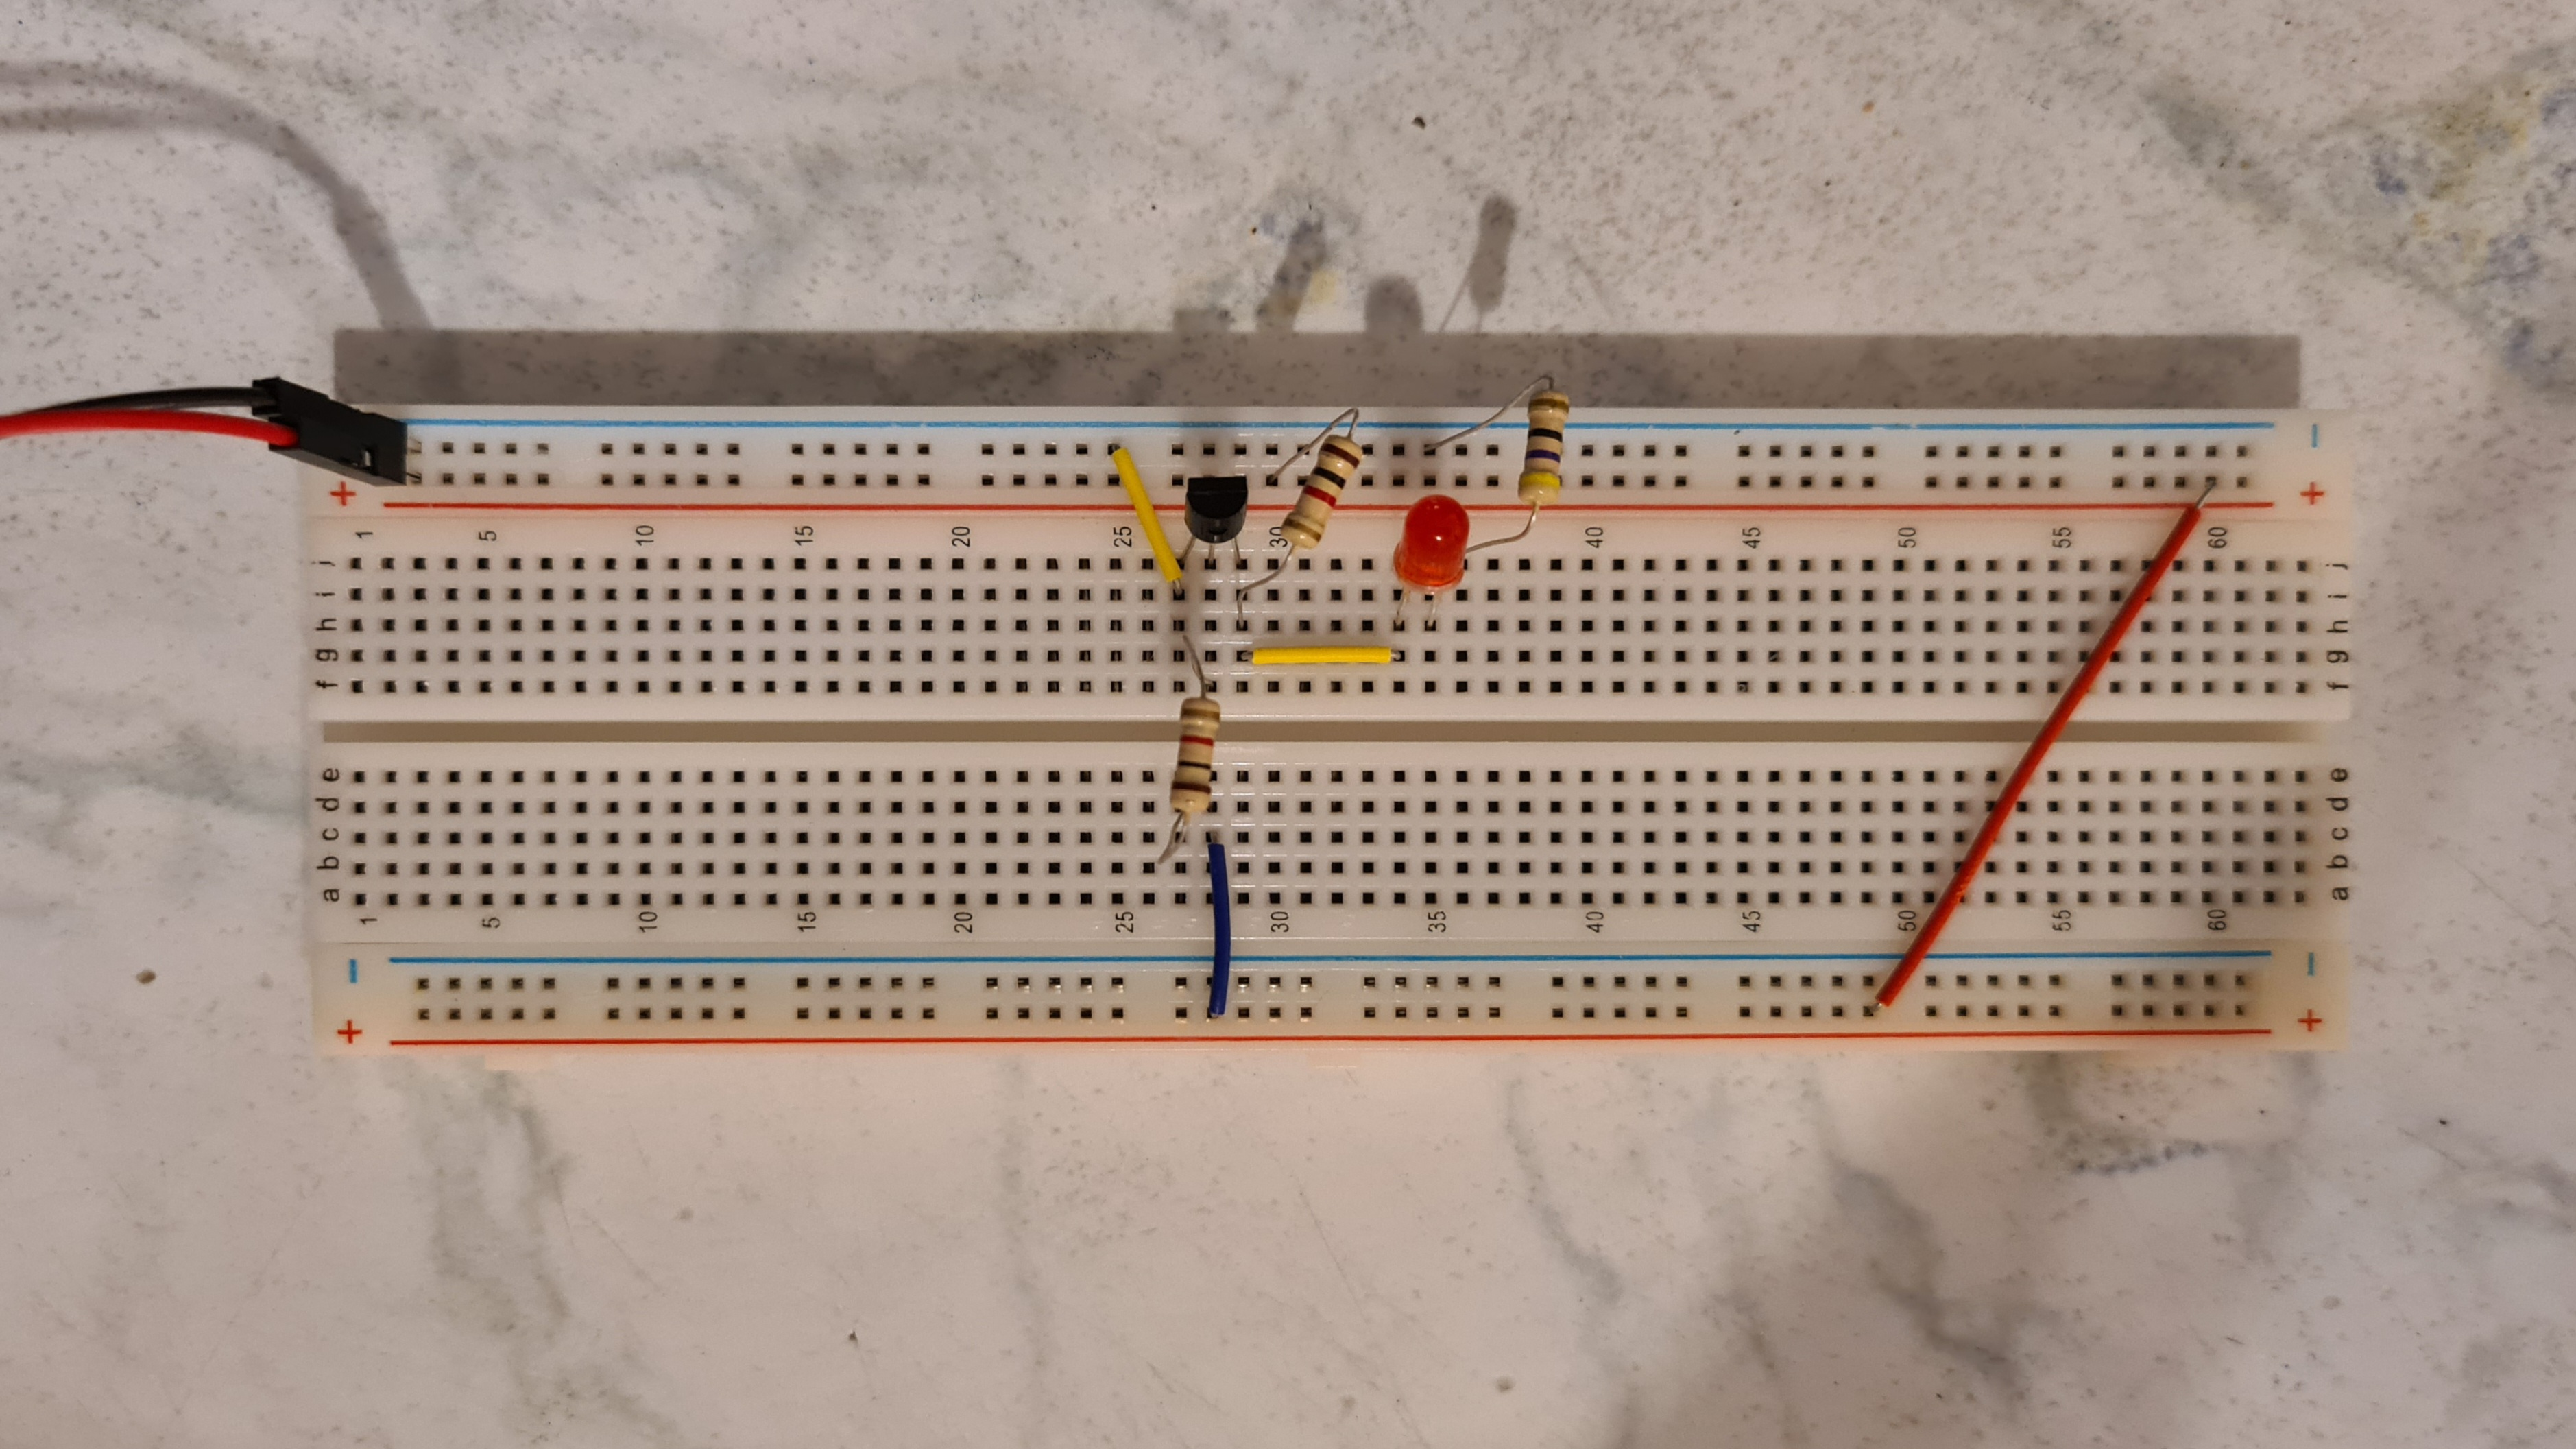
\includegraphics[height=4cm, keepaspectratio]{./Fotos/NICHT-1.jpg}
	\end{minipage}
	\caption{Praktischer Aufbau des NICHT-Gatters in allen möglichen Zuständen.}
\end{figure}
\newpage

\subsection{NAND-Gatter}
\begin{figure}[h]
	\centering
	\hspace{1cm}
	\begin{tabular}{|c|c|c|}
		\hline
		\textbf{A} & \textbf{B} & \textbf{Out} \\
		\hline
		0 & 0 & 1 \\
		1 & 0 & 1 \\
		0 & 1 & 1 \\
		1 & 1 & 0 \\
		\hline
	\end{tabular}
	\caption{Wahrheitstabelle für das logische NAND-Gatter}
\end{figure}
Wie in der Wahrheitstabelle zu erkennen, liegt Out auf HIGH, solange nicht A und B auf HIGH gesetzt sind. Das Verhalten dieses Gatters ist also gegenteilig zu dem des UND-Gatters. Der Name \gqq{NAND} setzt sich aus \gqq{NOT} und \gqq{AND} zusammen. Für das gewünschte Verhalten muss die Ausgabe eines UND-Gatters als Eingabe für ein NICHT-Gatter genutzt werden.\\
\begin{figure}[h!]
	\centering
	\begin{circuitikz}
		\draw (0, 0) node[npn](T1){$T_1$};
		\draw (0, -2) node[npn](T2){$T_2$};
		
		\draw (T1.B) to[R, l=$R_1$, a=\SI{2}{k\ohm}] ++(-2, 0) to[short, -o] ++(-.5, 0) node[left]{A};
		\draw (T2.B) to[R, l=$R_2$, a=\SI{2}{k\ohm}] ++(-2, 0) to[short, -o] ++(-.5, 0) node[left]{B};
		
		\draw (T1.C) to[short, -o] ++(0, 1) node[above]{$VCC$};
		\draw (T1.E) to[short] (T2.C);
		
		\draw (T2.E) to[R, l=$R_3$, a=\SI{330}{\ohm}] ++(0, -3) node[ground](GND){};
		
		\draw (5, -3) node[npn](T3){$T_3$};
		
		\draw (0, -3) to[short, *-] ++(1, 0) to[R, l=$R_4$, a=\SI{1}{k\ohm}] (T3.B);
		\draw (T3.E) to[short] ++(0, -1) node[ground](GND){};
		\draw (T3.C) to[short] ++(0, 1) to[R, l=$R_5$, a=\SI{1}{k\ohm}, -o] ++(0, 2) node[above]{$VCC$};
		
		\draw (5, -2) to[short, *-o] ++(2, 0) node[right]{Out};
		
		\draw[gray, very thick, densely dashed] (-3, 3) -- (6.5, 3) -- (6.5, -8) -- (-3, -8) -- cycle;
		\draw[lightgray, very thick, densely dashed] (-2.75, 2.75) -- (1.25, 2.75) -- (1.25, -6.75) -- (-2.75, -6.75) -- cycle;
		\draw[lightgray, very thick, densely dashed] (1.5, 2.75) -- (6.25, 2.75) -- (6.25, -6.75) -- (1.5, -6.75) -- cycle;
	
		\draw (6.5, -8) node[above right, gray]{NAND-Gatter};
		\draw (-.75, -6.75) node[below, gray]{UND-Gatter};
		\draw (3.875, -6.75) node[below, gray]{NICHT-Gatter};
	\end{circuitikz}
	\caption{Schaltplan für die logische NAND-Schaltung mithilfe von npn-Transistoren. Zusammengesetzt aus NICHT- und UND-Gatter.}
\end{figure}\\
Die Vorwiderstände an der Basis von $T_1$ und $T_2$ betragen hier jeweils $2\,k\Omega$, um den Stromfluss zwischen Basis und Emitter zu minimieren ($I_{BE} \approx 0.5\,mA$). Dies verhindert, dass durch $I_{BE}$ $T_3$ durchschaltet, wenn nur B auf HIGH liegt. Um zu verhindern, dass $U_{E,T2}$ zu sehr abfällt, wird dort gegen das Nullpotenzial ein Widerstand von $330\Omega$, statt $100\Omega$ verwendet. Der Aufbau des NICHT-Gatters bleibt unverändert.
\newpage
\begin{figure}[!h]
	\centering
	\hspace{1cm}
	\begin{tabular}{|c|c|c|}
		\hline
		\textbf{A} & \textbf{B} & $U_{BE,T_3}$ \\
		\hline
		0 & 0 & $0.0\,V$ \\
		1 & 0 & $0.0\,V$ \\
		0 & 1 & $0.3\,V$ \\
		1 & 1 & $1.0\,V$ \\
		\hline
	\end{tabular}
	\caption{Messwerte der Basis-Emitter-Spannung von $T_3$ für alle möglichen Zustände von A und B im NAND-Gatter.}
\end{figure}
Wenn A oder B auf LOW gesetzt ist, wird die Basis von $T_3$ durch $R_3$ und $R_4$ auf dass Nullniveau gesenkt. Ist nur B auf HIGH gesetzt, so liegt wegen $I_{BE,T2}$ an der Basis von $T_3$ eine kleine Spannung $U_{BE,T_3} \approx 0.3\,V$ an. Diese genügt jedoch nicht, um den Transistor durchzuschalten. Erst wenn A und B auf HIGH liegen, fällt durch $T_3$ die Spannung an Out ab.\\
\begin{figure}[h!]
	\begin{minipage}{.5\textwidth}
		\centering
		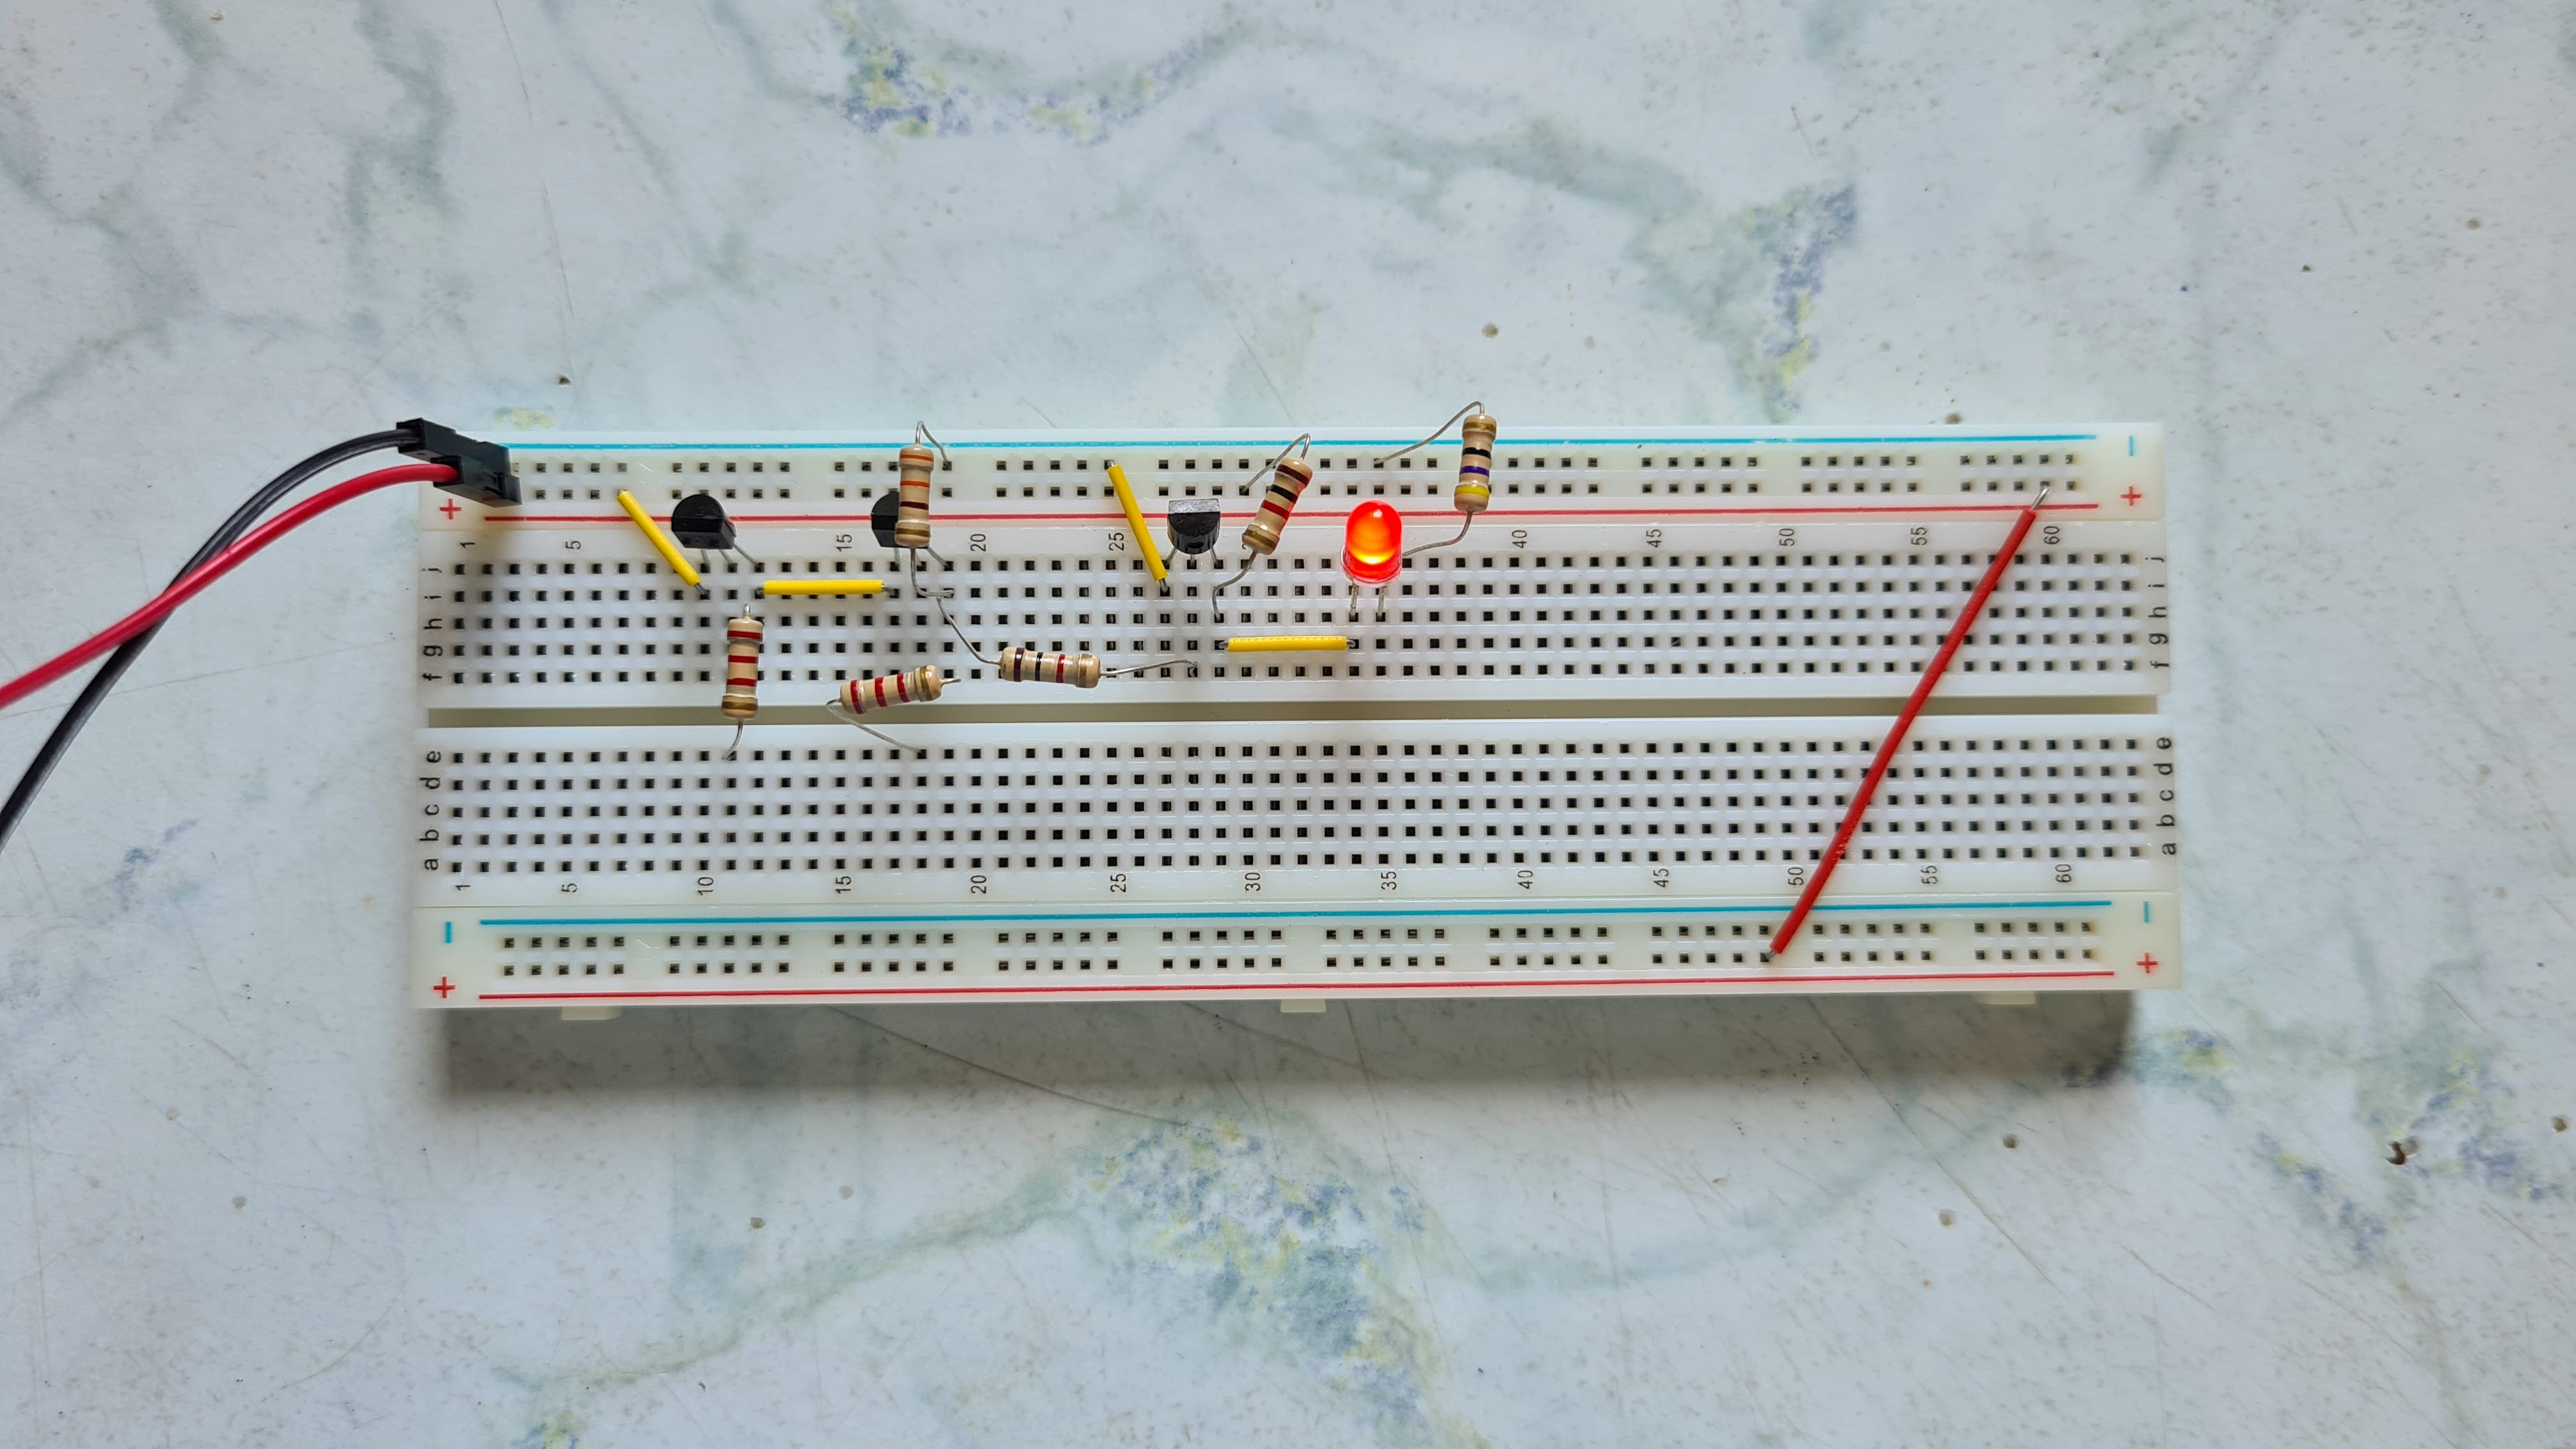
\includegraphics[height=4cm, keepaspectratio]{./Fotos/NAND-00.jpg}
		\vspace{1cm}
	\end{minipage}%
	\begin{minipage}{.5\textwidth}
		\centering
		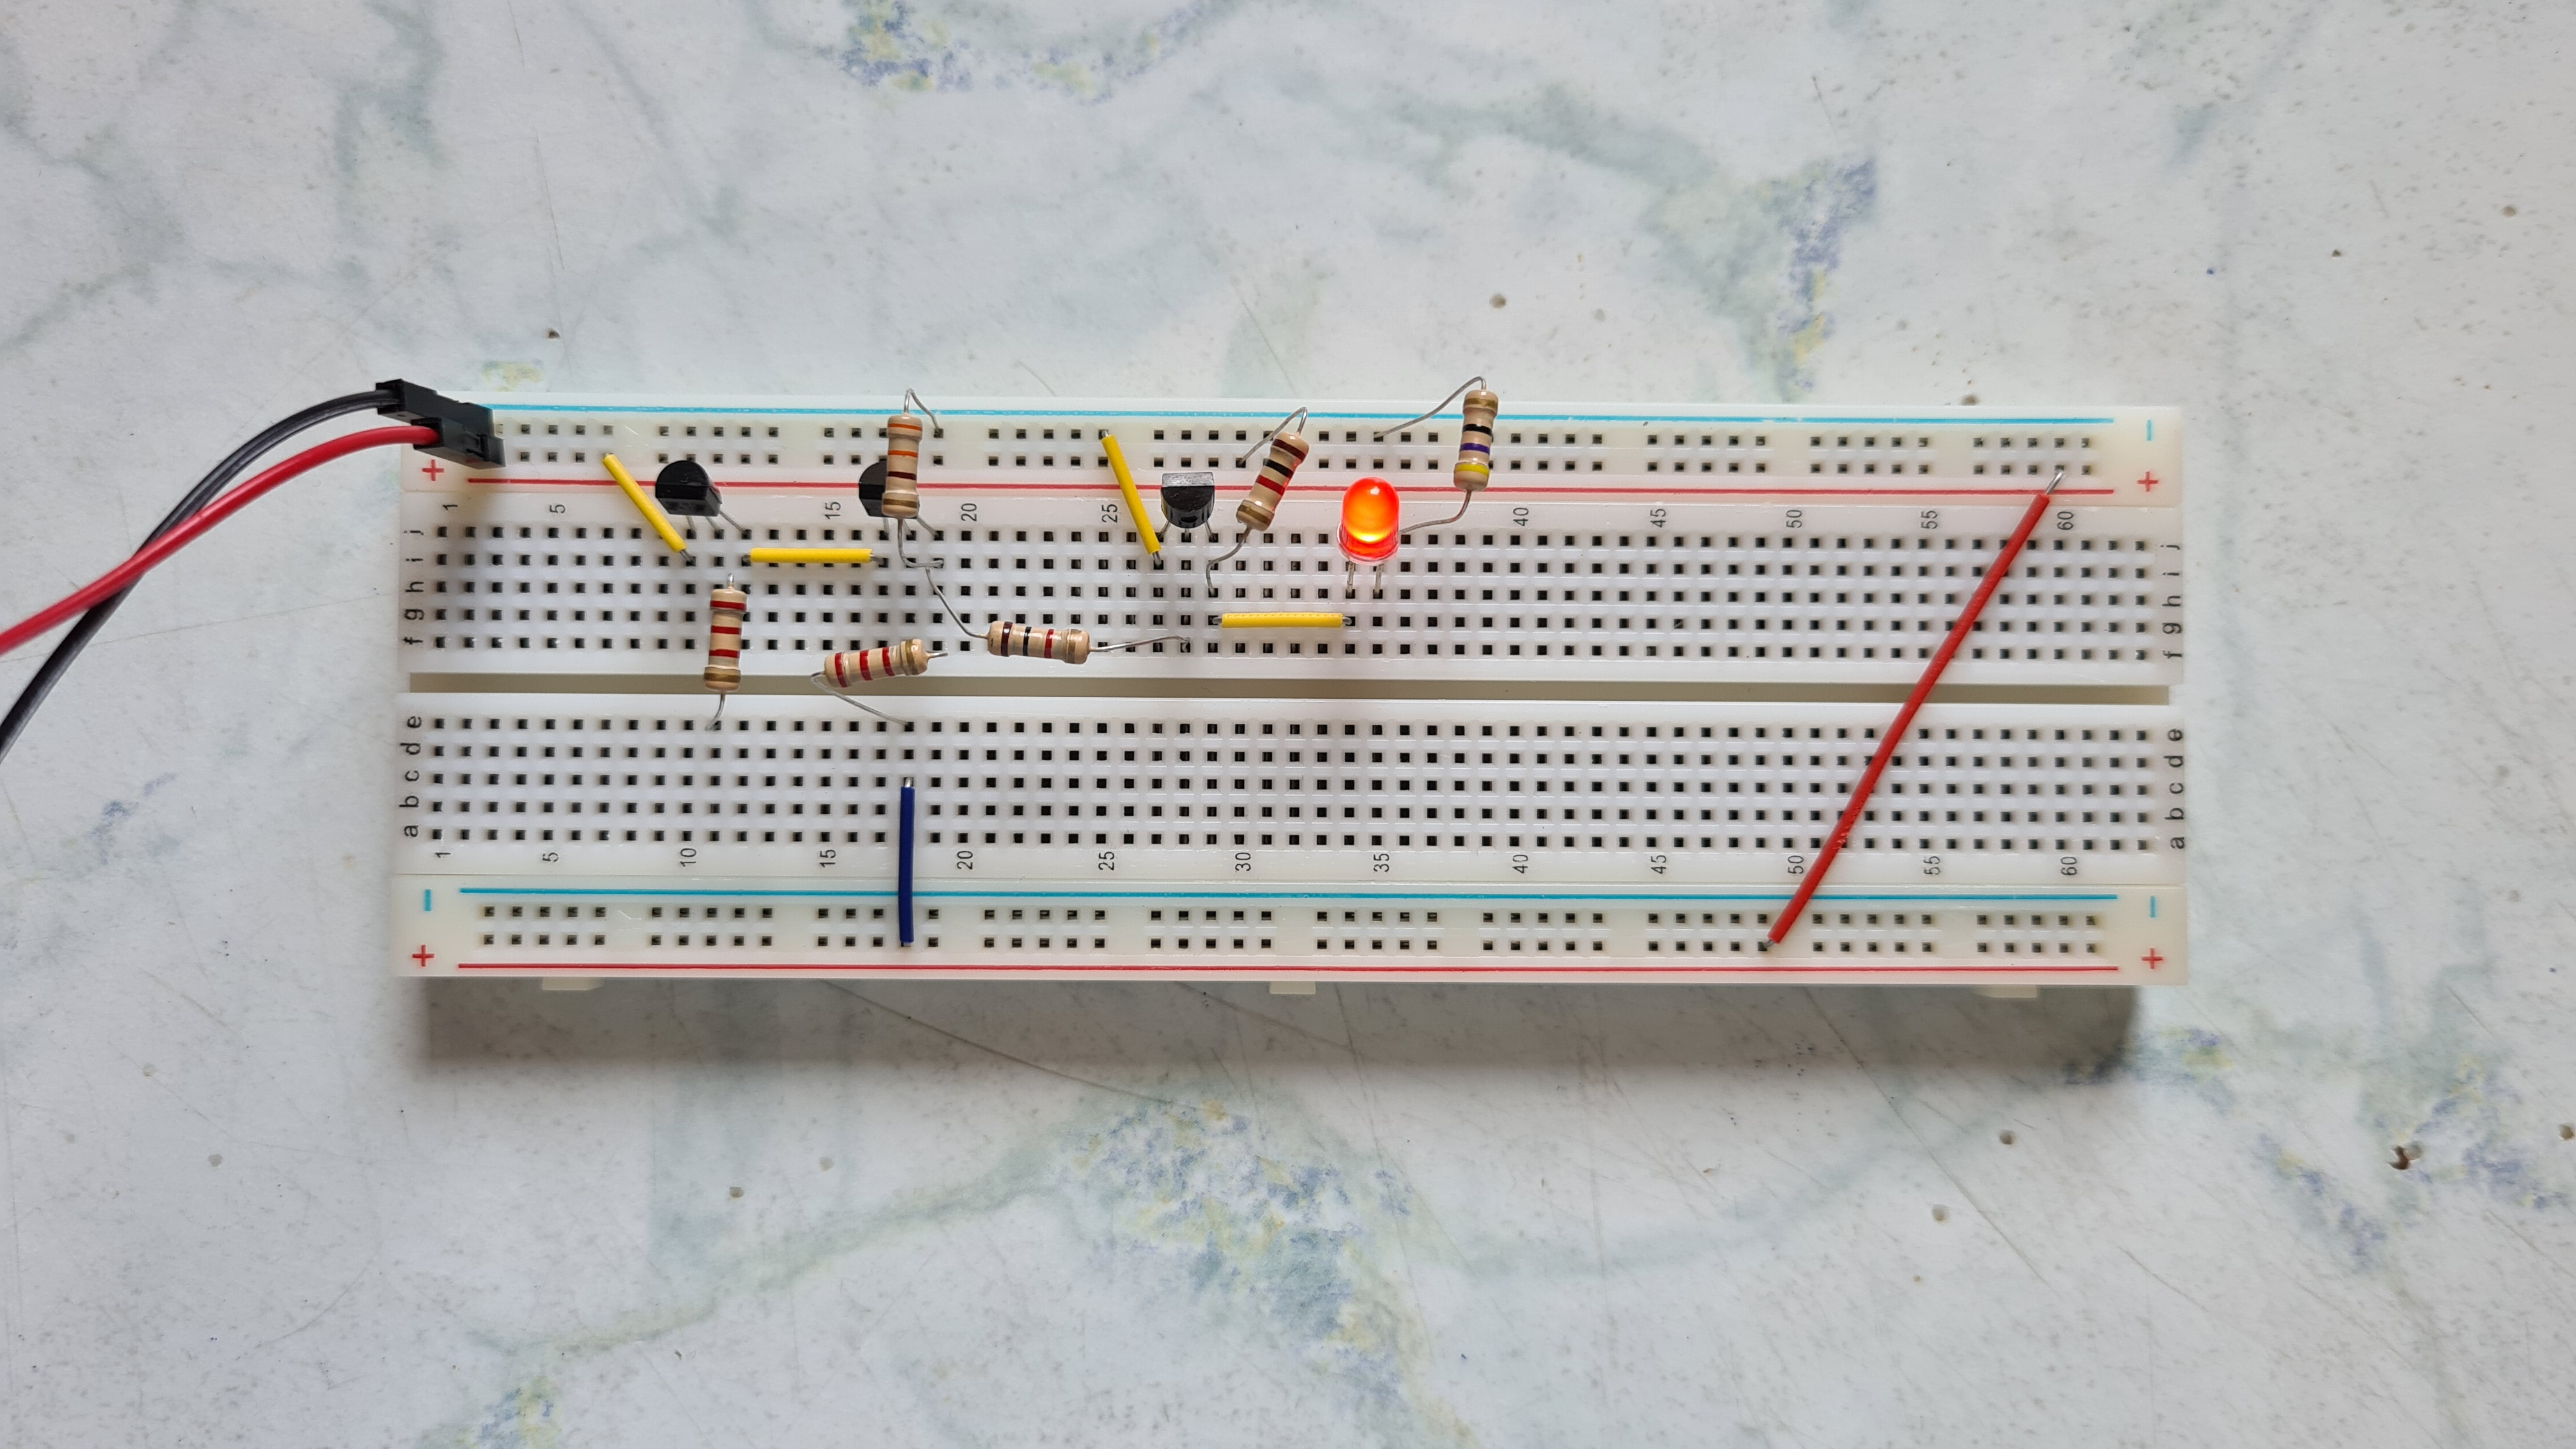
\includegraphics[height=4cm, keepaspectratio]{./Fotos/NAND-01.jpg}
		\vspace{1cm}
	\end{minipage}
	\begin{minipage}{.5\textwidth}
		\centering
		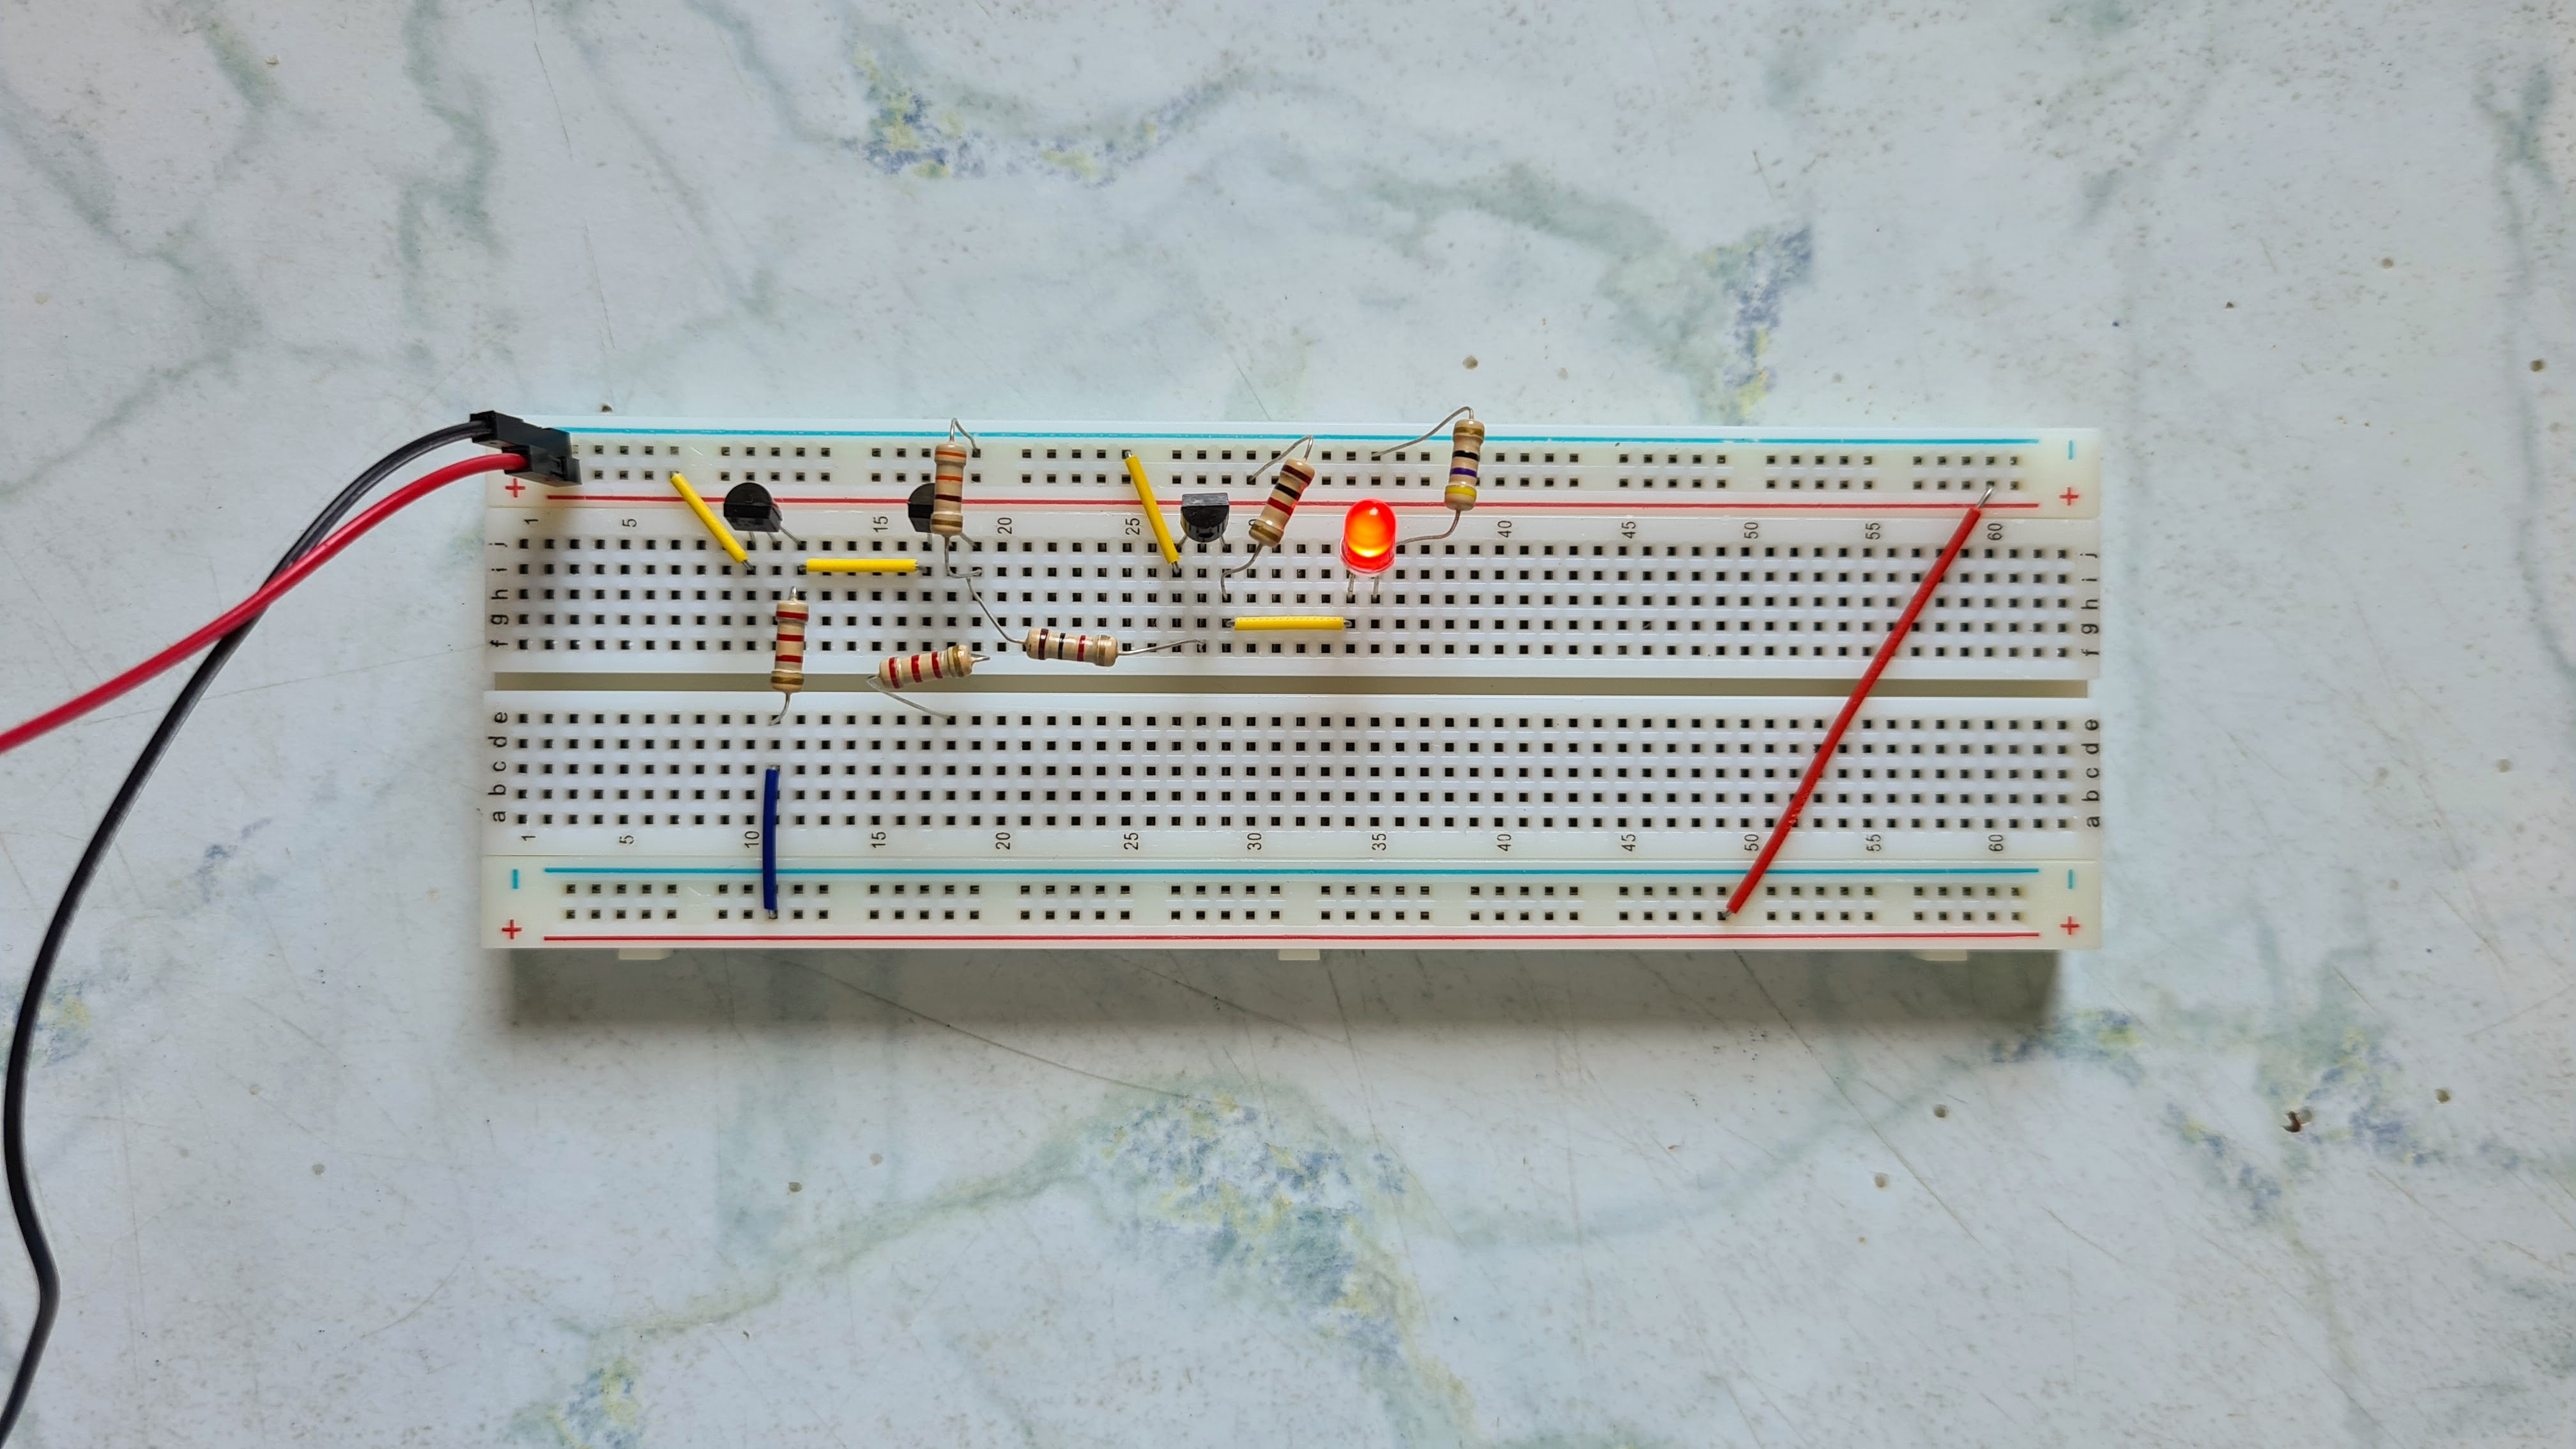
\includegraphics[height=4cm, keepaspectratio]{./Fotos/NAND-10.jpg}
	\end{minipage}%
	\begin{minipage}{.5\textwidth}
		\centering
		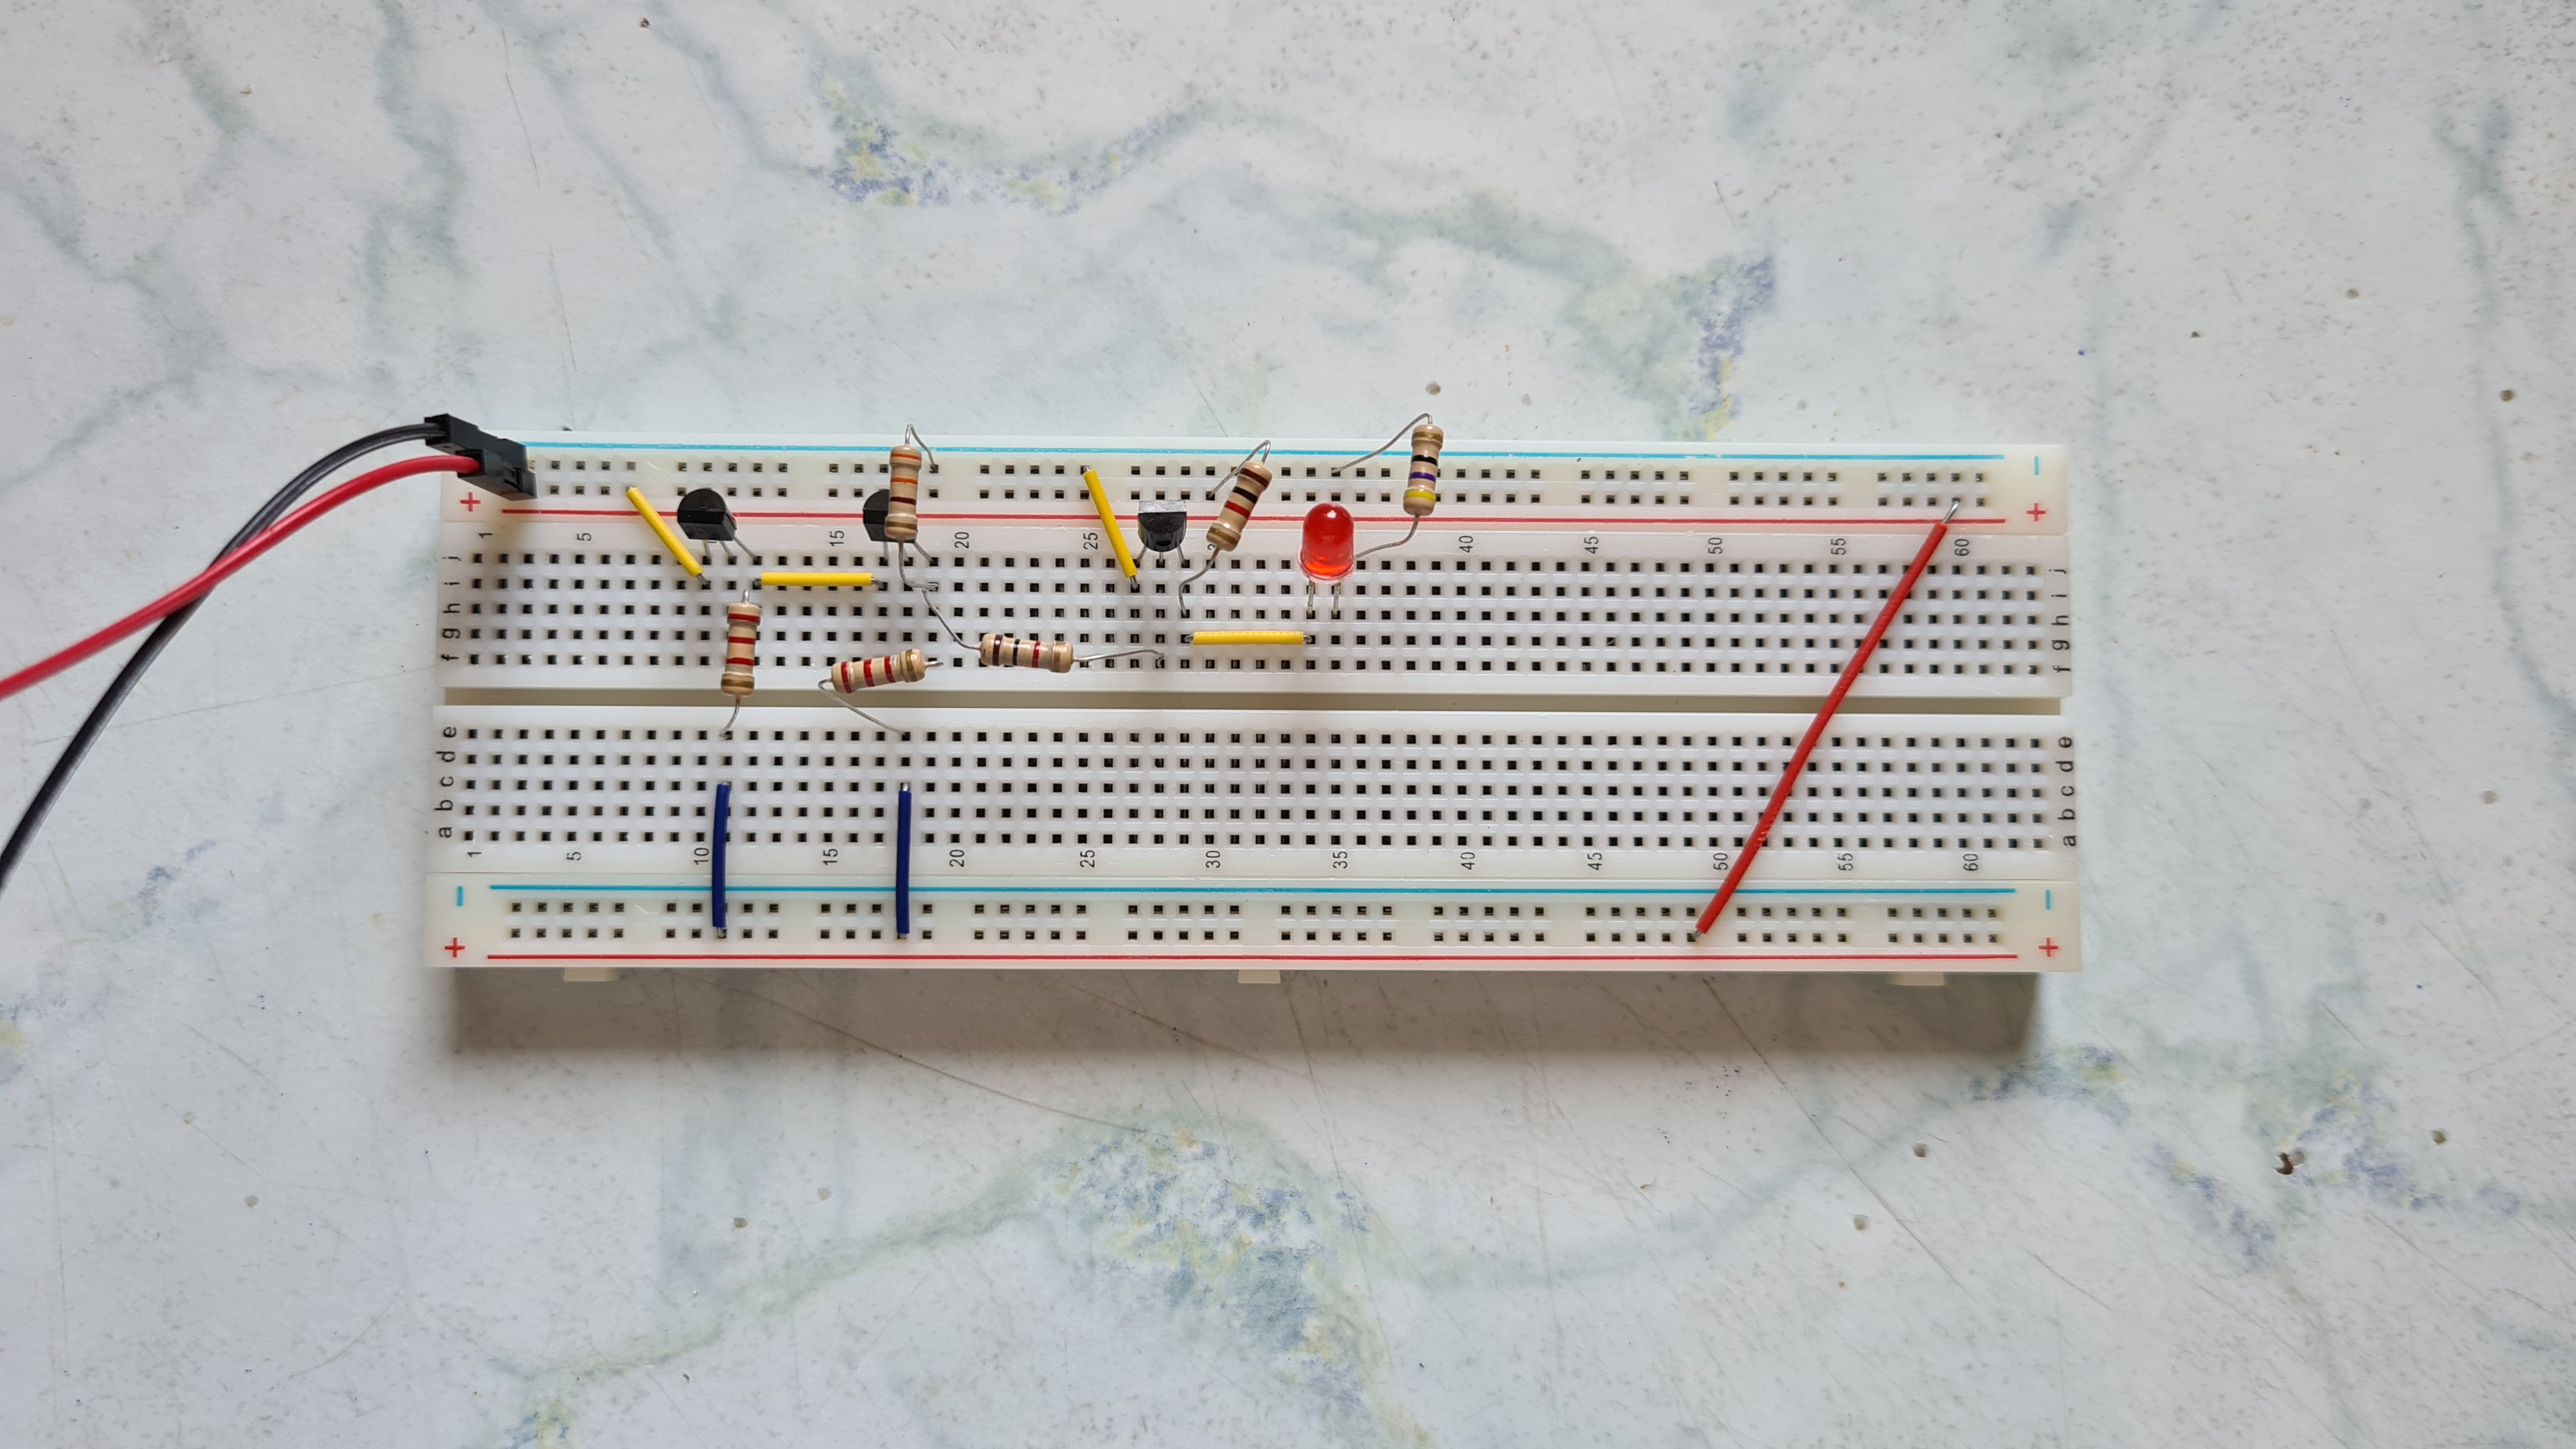
\includegraphics[height=4cm, keepaspectratio]{./Fotos/NAND-11.jpg}
	\end{minipage}
	\caption{Praktischer Aufbau des NAND-Gatters in allen möglichen Zuständen.}
\end{figure}

\subsection{EXOR-Gatter} \label{EXOR}
\begin{figure}[h]
	\centering
	\hspace{1cm}
	\begin{tabular}{|c|c|c|}
		\hline
		\textbf{A} & \textbf{B} & \textbf{Out} \\
		\hline
		0 & 0 & 0 \\
		1 & 0 & 1 \\
		0 & 1 & 1 \\
		1 & 1 & 0 \\
		\hline
	\end{tabular}
	\caption{Wahrheitstabelle für das logische EXOR-Gatter}
\end{figure}
Der Name des EXOR-Gatters leitet sich aus \gqq{exclusive or} (= ausschließendes ODER) ab. Hierbei ist Out also nur dann auf HIGH, wenn ausschließlich A oder B auf HIGH liegen. Sind A und B auf HIGH, liegt Out auf LOW. Anders ausgedrückt ist Out immer dann auf HIGH, wenn A und B unterschiedliche Zustände aufweisen. Setzt man das EXOR-Gatter aus mehreren kleineren Gattern zusammen, so kann als Grundlage das ODER-Gatter verwendet werden. Dieses verhält bereits sich in drei der vier möglichen Fälle richtig. Sind A und B auf HIGH, muss Out auf Low liegen. Es muss also \gqq{A ODER B} zutreffen, nicht jedoch \gqq{A UND B}. Es ergibt sich der logische Ausdruck \gqq{(A ODER B) UND (A NAND B)}.\\
\begin{figure}[h!]
	\centering
	\begin{circuitikz}
		
		% OR
		
		\draw (0, 0) node[npn](T1){$T_1$};
		\draw (1, -2) node[npn](T2){$T_2$};
		
		\draw (T1.B) to[R, l=$R_1$, a=\SI{2}{k\ohm}] (-3, 0) to[short, -o] ++(-2, 0) node[left]{A};
		\draw (T2.B) to[R, l=$R_2$, a=\SI{2}{k\ohm}] (-3, -2) to[short, -o] ++(-2, 0) node[left]{B};
		
		\draw (T1.C) to[short, *-] ++(1, 0) to[short] (T2.C);
		\draw (T1.C) to[short, -o] (0, 2) node[above]{$VCC$};
		\draw (T1.E) to[short] ++(2, 0) to[short, -*] (2, -3);
		
		\draw (T2.E) to[short] (1, -3) to[short] (2, -3) to[R, l=$R_3$, a=\SI{330}{\ohm}] (2, -5) node[ground]{};
		
		
		\draw[lightgray, very thick, densely dashed] (-3, 3) -- (3, 3) -- (3, -6) -- (-3, -6) -- cycle;
		\draw (0, -6) node[below, gray]{ODER-Gatter};
		
		% NAND
		
		\draw (0, -9) node[npn](T3){$T_3$};
		\draw (0, -11) node[npn](T4){$T_4$};
		
		\draw (T3.C) to[short, -o] (0, -8) node[above]{$VCC$};
		\draw (T3.E) to[short] (T4.C);
		
		\draw (T3.B) to[R, l=$R_4$, a=\SI{2}{k\ohm}] (-3, -9) to[short] ++(-.5, 0) to[short, -*] (-3.5, 0);
		\draw (T4.B) to[R, l=$R_5$, a=\SI{2}{k\ohm}] (-3, -11) to[short] ++(-1, 0) to[short, -*] (-4, -2);
		
		\draw (T4.E) to[R, l=$R_6$, a=\SI{330}{\ohm}] (0, -14) node[ground]{};
		
		\draw (3, -12) node[npn](T5){$T_5$};
		\draw (T5.B) to[R, l=$R_7$, a=\SI{1}{k\ohm}, -*] (0, -12);
		\draw (T5.E) to[short] (3, -14) node[ground]{};
		
		\draw (T5.C) to[short] (3, -10) to[R, l=$R_8$, a=\SI{1}{k\ohm}, -o] (3, -8) node[above]{$VCC$};
		

		\draw[lightgray, very thick, densely dashed] (-3, -7) -- (5, -7) -- (5, -15) -- (-3, -15) -- cycle;
		\draw (1, -15) node[below, gray]{NAND-Gatter};
		
		% UND
		
		\draw (8, 0) node[npn](T6){$T_6$};
		\draw (8, -2) node[npn](T7){$T_7$};
		
		\draw (T6.C) to[short, -o] (8, 2) node[above]{$VCC$};
		\draw (T6.E) to[short] (T7.C);
		
		\draw (T6.B) to[R, l=$R_9$, a=\SI{1}{k\ohm}] (5, 0) to[short] (5, -3) to[short] (2, -3);
		\draw (T7.B) to[R, l=$R_{10}$, a=\SI{1}{k\ohm}] (5.5, -2) to[short] (5.5, -11) to[short, -*] (3, -11);
		
		\draw (T7.E) to[R, l=$R_{11}$, a=\SI{100}{\ohm}] (8, -5) node[ground]{};
		\draw (8, -3) to[short, *-o] (11, -3) node[right]{Out};
		
		\draw[lightgray, very thick, densely dashed] (4, 3) -- (9.5, 3) -- (9.5, -6) -- (4, -6) -- cycle;
		\draw (6.75, -6) node[below, gray]{UND-Gatter};
		
		\draw[gray, very thick, densely dashed] (-4.5, 3.5) -- (10, 3.5) -- (10, -16) -- (-4.5, -16) -- cycle;
		\draw (10, -16) node[above right, gray]{EXOR-Gatter};
		
	\end{circuitikz}
	\caption{Unoptimierter Schaltplan für die logische EXOR-Schaltung mithilfe von npn-Transistoren. Zusammengesetzt aus NAND-, ODER- und UND-Gatter.}
\end{figure}\\
\newpage
Bei der Verkettung von UND-, ODER- und NAND-Gattern ergibt sich der abgebildete Schaltplan. Um diesen zu Realisieren wären insgesamt sieben Transistoren nötig. Die Ausgänge des ODER- und NAND-Gatters werden mit den Eingängen A und B des UND-Gatters verbunden.\\\\
Beim Versuch diese Schaltung praktisch umzusetzen ergaben sich allerdings einige Probleme. Oftmals wies die Schaltung unerwünschtes Verhalten auf. Die Fehlerquelle zu bestimmen erwies sich aufgrund der Größe ebenfalls als schwierig. Nicht zuletzt ist es aus Platz- und Kostengründen nicht zu wünschen Schaltungen unnötig groß zu gestalten. Es galt also, die Schaltung weitmöglichst zu vereinfachen.\\\\
Die erste Optimierungsmöglichkeit fand sich im NAND-Gatter. Dessen Aufbau setzte sich zuletzt aus drei Transistoren zusammen. Davon bildeten zwei ein logisches UND-Gatter, der Übrige ein NICHT-Gatter. Durch die Verbindung dieser beiden Gatter wurde das Verhalten eines UND-Gatters invertiert. Jedoch ist es möglich, dieses Ergebnis mit nur zwei Transistoren zu reproduzieren. Hierfür liegt Out über einen Widerstand an der Versorgungsspannung. Über zwei Transistoren wird Out zusätzlich mit dem Nullpotenzial verbunden. Analog zum UND-Gatter liegen A und B jeweils an der Basis von einem der beiden Transistoren. Ist mindestens einer der Eingänge auf LOW, ist die Verbindung zwischen Out und dem Nullpotenzial unterbrochen, wodurch Out auf HIGH liegt. Sind A und B auf HIGH, so fällt die Spannung an Out über die beiden Transistoren ab. Somit liegt Out auf LOW.\\
\begin{figure}[h!]
	\centering
	\begin{circuitikz}
		\draw (0, 0) node[npn](T1){$T_1$};
		\draw (0, -2) node[npn](T2){$T_2$};
		
		\draw (T1.B) to[R, l=$R_1$, a=\SI{2}{k\ohm}] ++(-2, 0) to[short, -o] ++(-.5, 0) node[left]{A};
		\draw (T2.B) to[R, l=$R_2$, a=\SI{2}{k\ohm}] ++(-2, 0) to[short, -o] ++(-.5, 0) node[left]{B};
		
		\draw (T1.E) to[short] (T2.C);
		
		\draw (T1.C) to[R, l=$R_3$, a=\SI{1}{k\ohm}, -o] (0, 3) node[above]{$VCC$};
		\draw (T1.C) to[short, *-o] ++(2, 0) node[right]{Out};
		
		\draw (T2.E) to[short] (0, -3) node[ground]{};
		
		\draw[gray, very thick, densely dashed] (-3, 4) -- (1.5, 4) -- (1.5, -4) -- (-3, -4) -- cycle;
		\draw (1.5, -4) node[above right, gray]{NAND-Gatter};
	\end{circuitikz}
	\caption{Optimierter Schaltplan für die logische NAND-Schaltung, bestehend aus lediglich zwei Transistoren.}
\end{figure}\\
Durch diese Vereinfachung kann zwar auf einen Transistor verzichtet werden, jedoch sind noch immer insgesamt sechs für den Bau des EXOR-Gatters nötig. Das verwenden eines UND-Gatters, um Out auf LOW zu ziehen, kann allerdings auch beim EXOR-Gatter angewandt werden.\\\\
In drei der vier möglichen Zustände des ODER-Gatters ist Out auf HIGH. Sind A und B auf HIGH, so soll allerdings Out auf LOW liegen. Analog zum optimierten NAND-Gatter können hier zwei Transistoren genutzt werden. Diese werden in Reihe geschaltet und verbinden den Ausgang des ODER-Gatters mit dem Nullpotenzial. Hierbei ist Out auf HIGH, sobald entweder A oder B auf HIGH ist. Sind A und B auf HIGH, so schalten die beiden Transistoren durch und die Spannung an Out fällt ab. Somit verhält sich das EXOR-Gatter in allen vier Zuständen richtig.\\
\begin{figure}[h!]
	\centering
	\begin{circuitikz}
		\draw (0, 0) node[npn](T1){$T_1$};
		\draw (2, -2) node[npn](T2){$T_2$};
		
		\draw (T1.B) to[R, l=$R_1$, a=\SI{2}{k\ohm}] ++(-2, 0) to[short] ++(-1, 0) to[short, -o] ++(-1, 0) node[left]{A};
		\draw (T2.B) to[R, l=$R_2$, a=\SI{2}{k\ohm}] ++(-4, 0) to[short] ++(-1, 0) to[short, -o] ++(-1, 0) node[left]{B};
		
		\draw (T1.C) to[short, -o] (0, 2) node[above]{$VCC$};
		\draw (T2.C) to[short] ++(0, 2) to[short, -*] ++(-2, 0);
		
		\draw (T1.E) to[short] ++(3, 0) to[short, -*] (3, -3);
		\draw (T2.E) to[short] (2, -3) to[short, -o] (5, -3) node[right]{Out};
		
		\draw (3, -4) node[npn](T3){$T_3$};
		\draw (3, -6) node[npn](T4){$T_4$};
		
		\draw (T3.C) to[short] (3, -3);
		\draw (T3.E) to[short] (T4.C);
		\draw (T4.E) to[short] (3, -7) node[ground]{};
		
		\draw (T3.B) to[R, l=$R_3$, a=\SI{2}{k\ohm}] ++(-2, 0) to[short] (-3.5, -4) to[short, -*] (-3.5, 0);
		\draw (T4.B) to[R, l=$R_4$, a=\SI{2}{k\ohm}] ++(-2, 0) to[short] (-3, -6) to[short, -*] (-3, -2);
		
		\draw[gray, very thick, densely dashed] (-4, 3) -- (4, 3) -- (4, -8) -- (-4, -8) -- cycle;
		\draw (4, -8) node[above right, gray]{EXOR-Gatter};
		
	\end{circuitikz}
	\caption{Optimierter Schaltplan für die logische EXOR-Schaltung, bestehend aus lediglich vier Transistoren.}
\end{figure}
\begin{figure}[h!]
	\begin{minipage}{.5\textwidth}
		\centering
		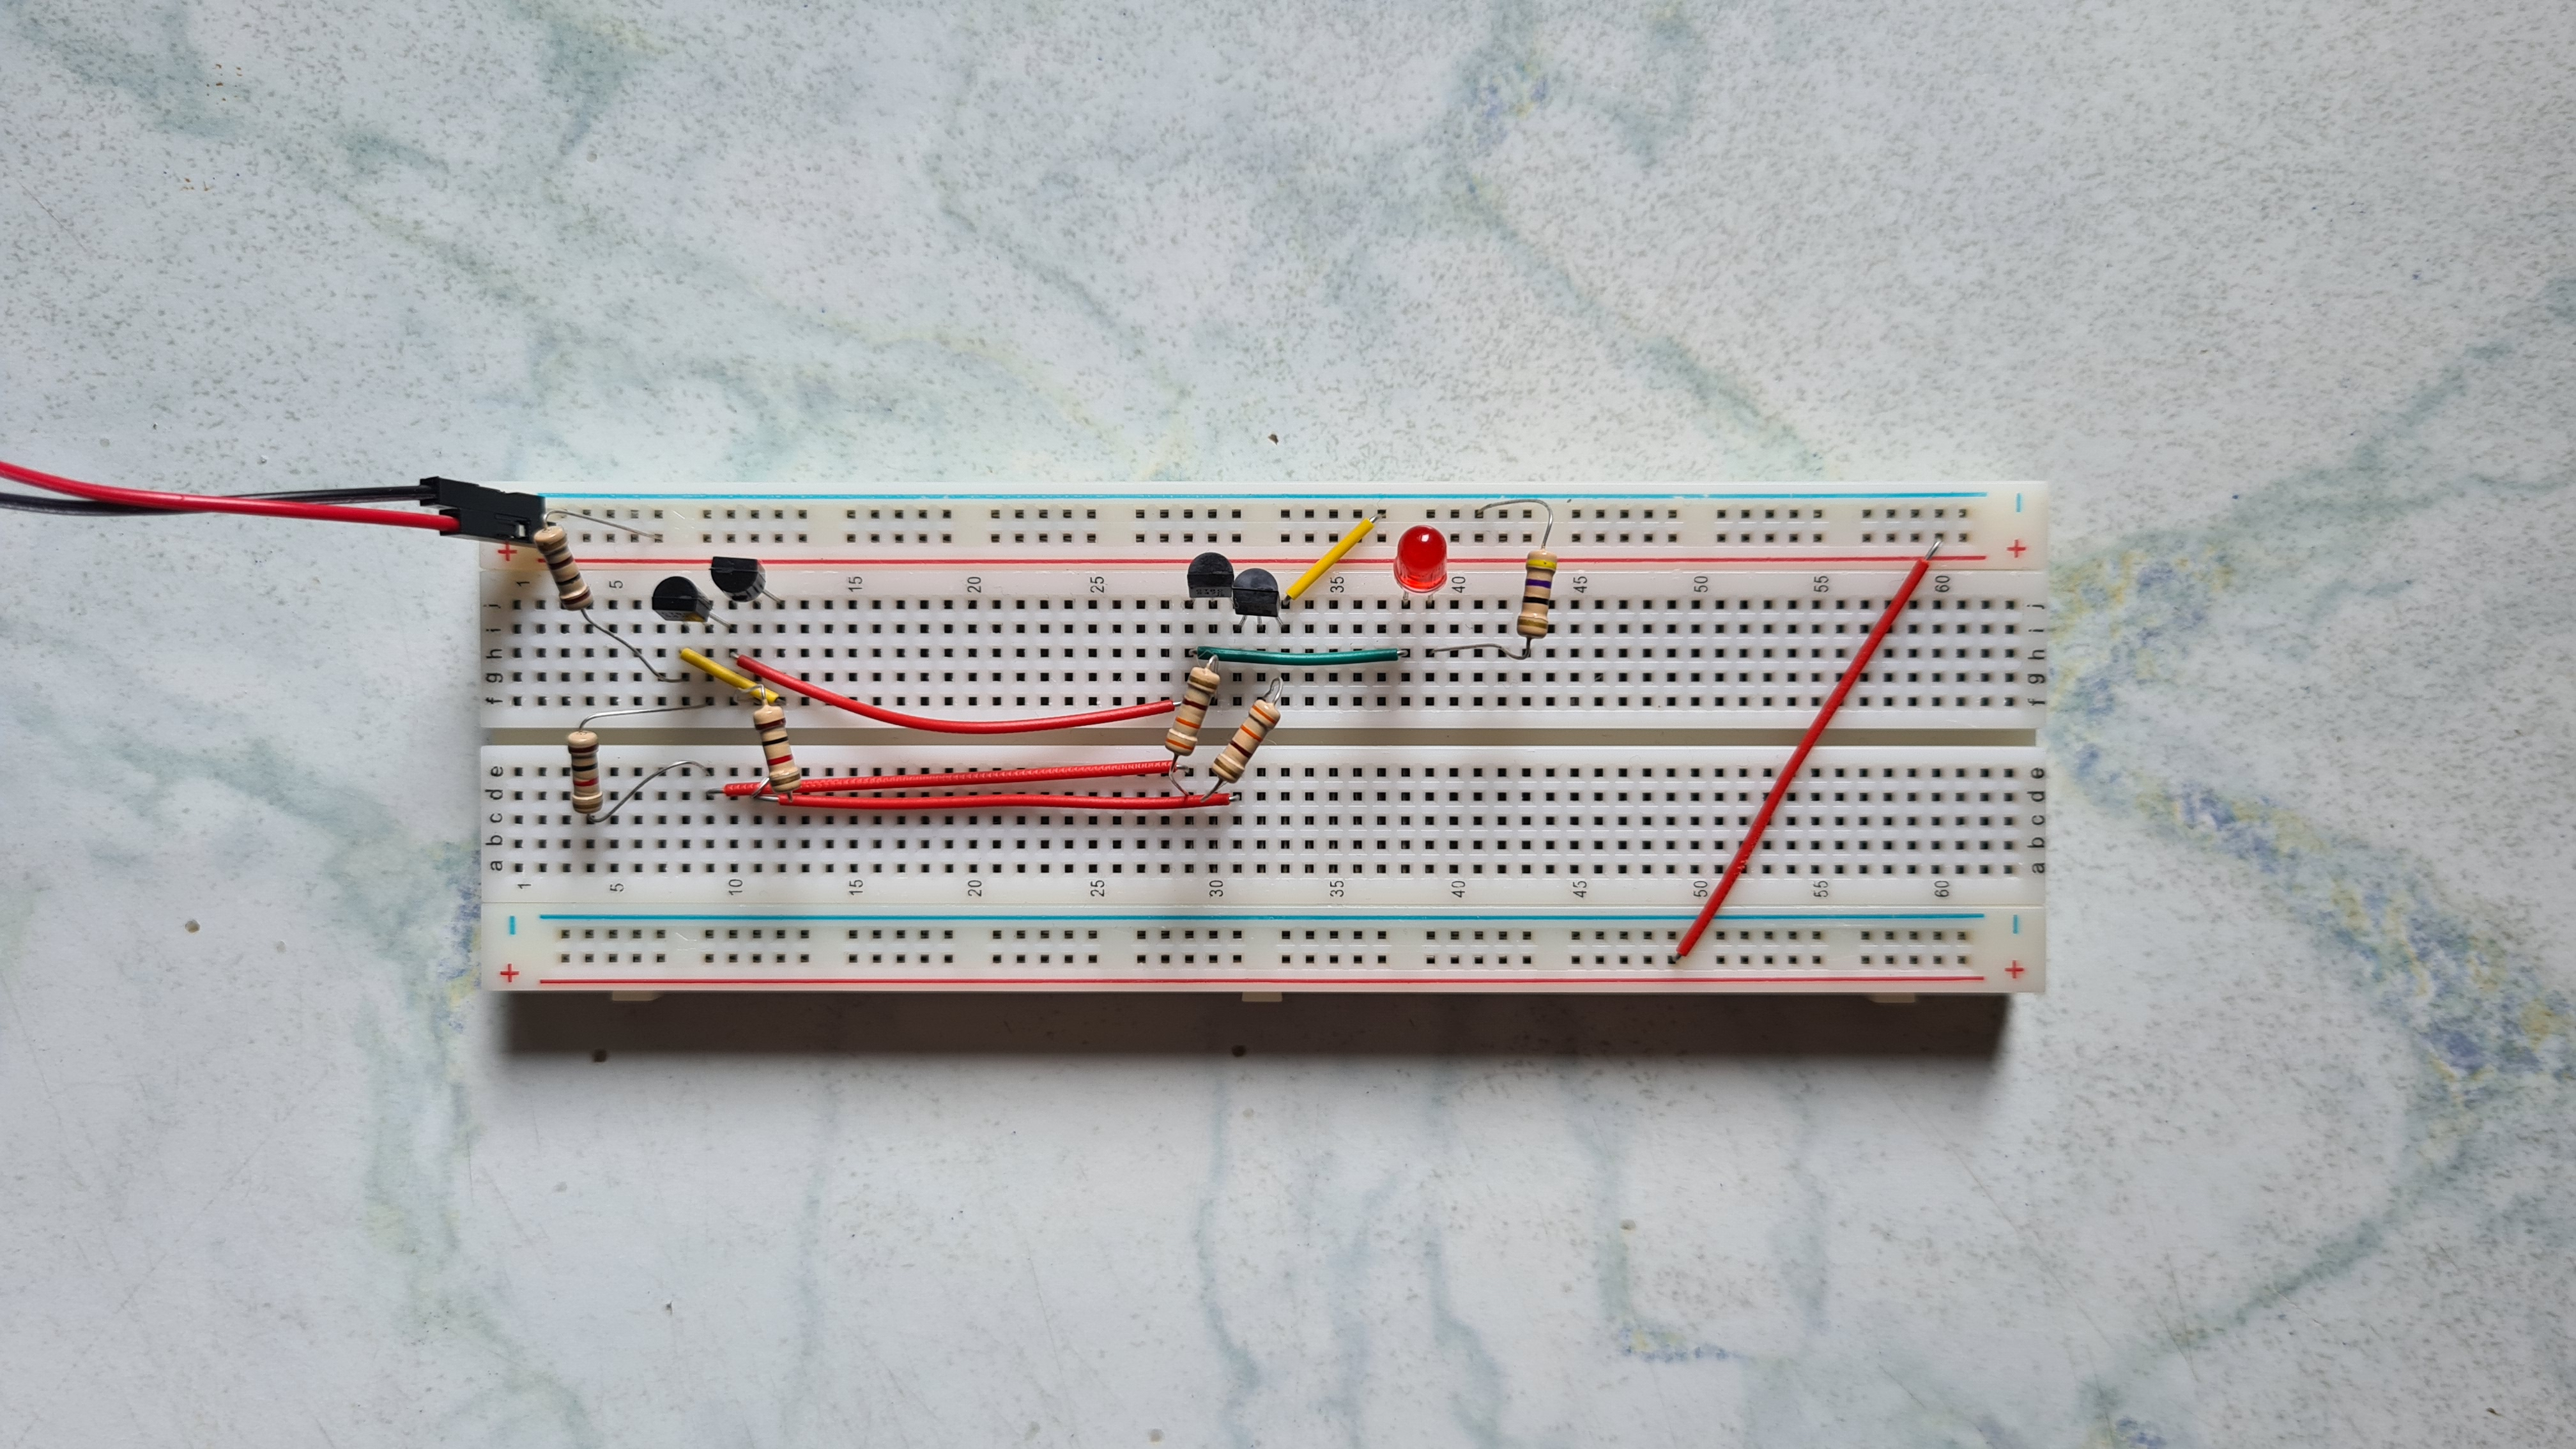
\includegraphics[height=4cm, keepaspectratio]{./Fotos/EXOR-00.jpg}
		\vspace{1cm}
	\end{minipage}%
	\begin{minipage}{.5\textwidth}
		\centering
		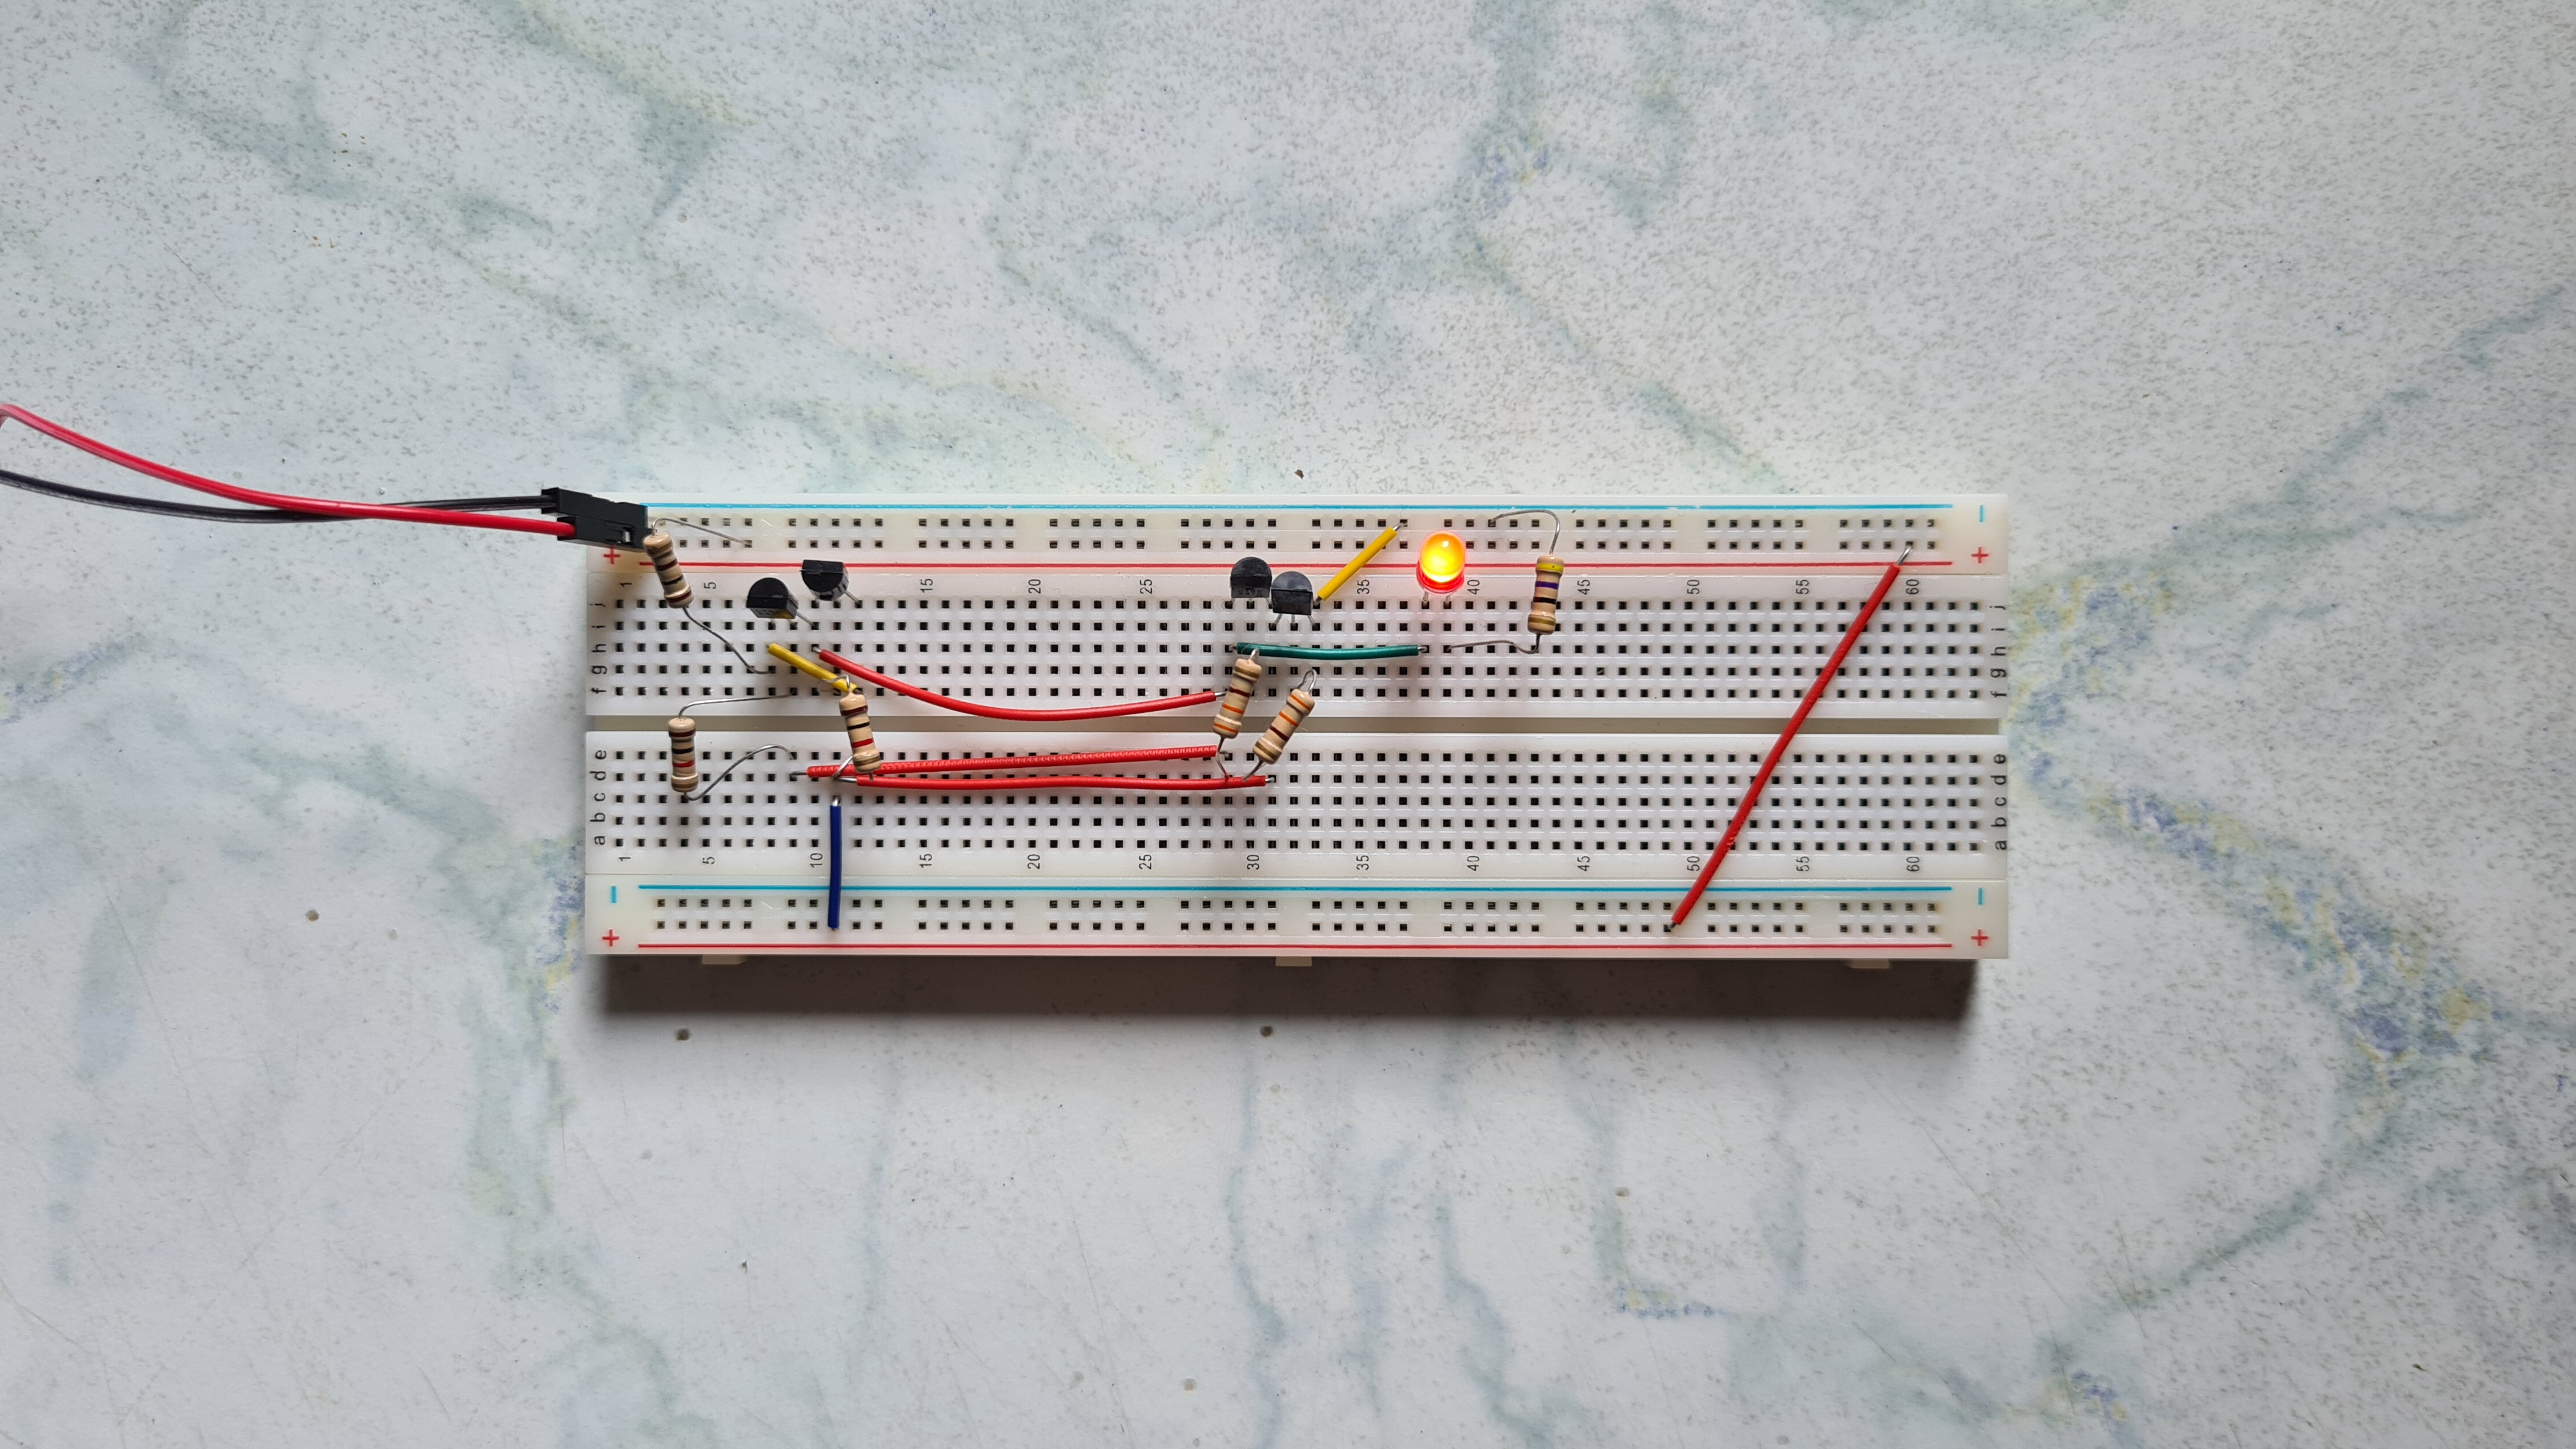
\includegraphics[height=4cm, keepaspectratio]{./Fotos/EXOR-01.jpg}
		\vspace{1cm}
	\end{minipage}
	\begin{minipage}{.5\textwidth}
		\centering
		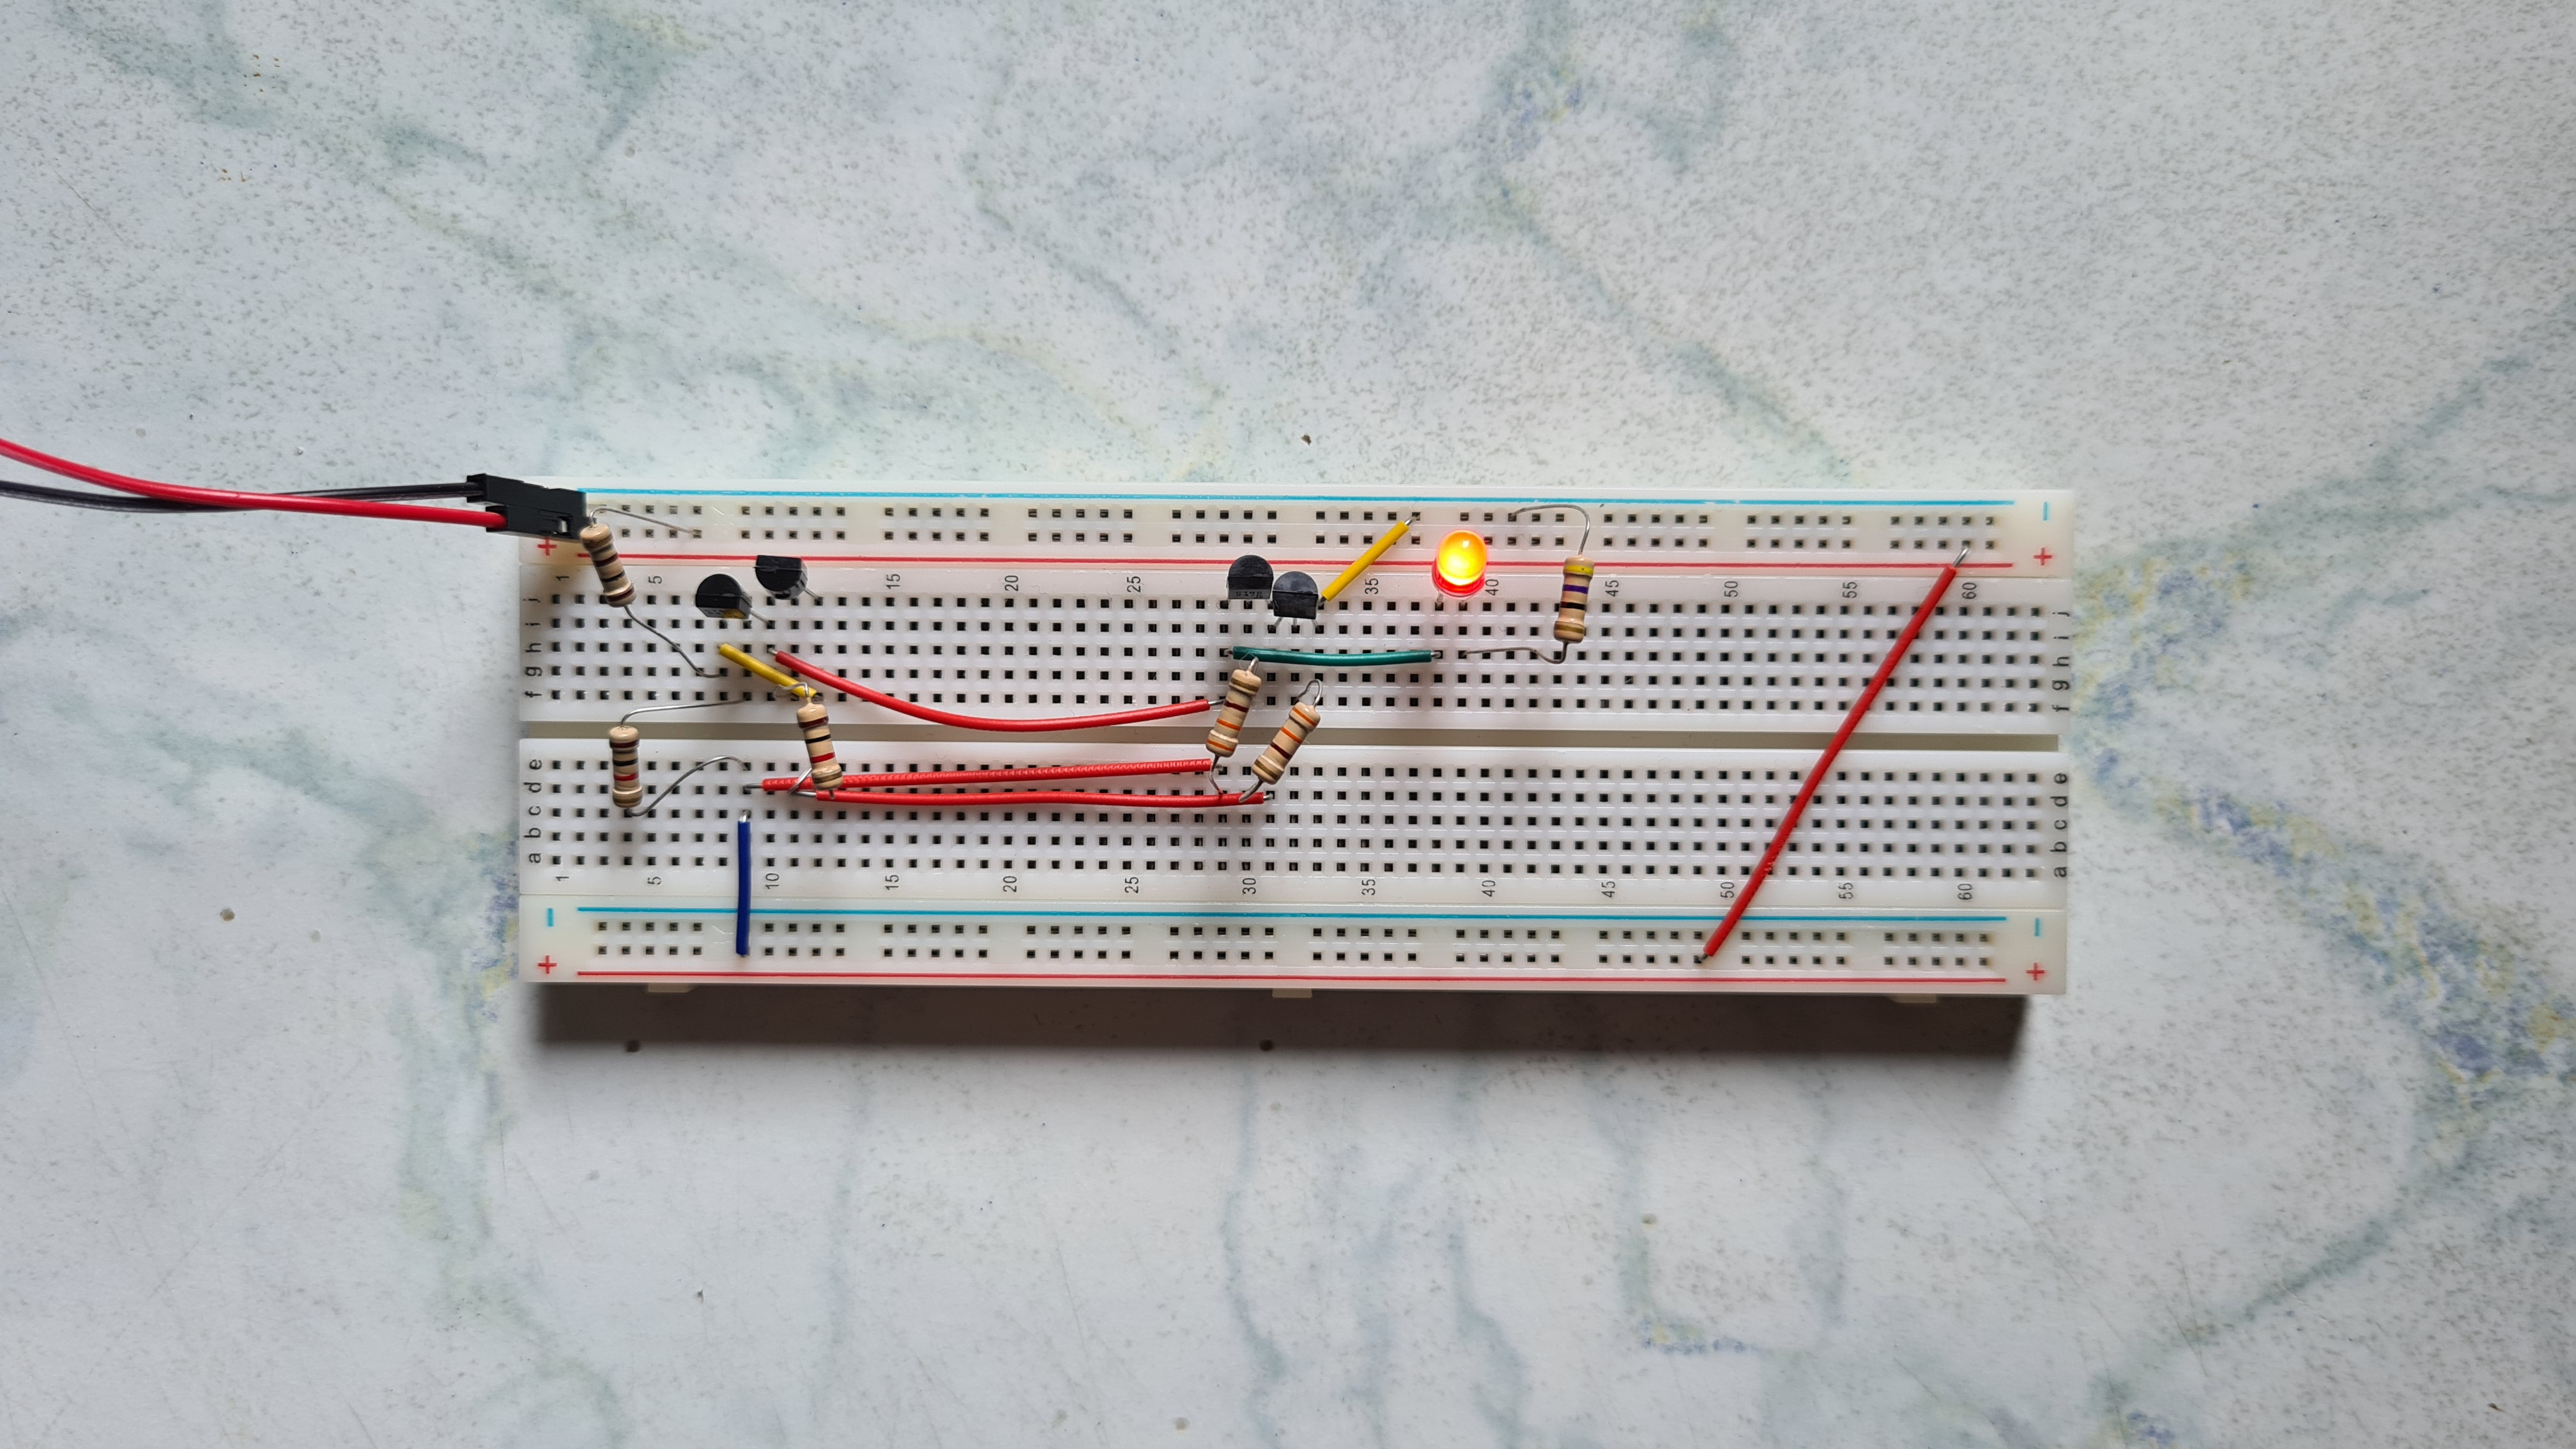
\includegraphics[height=4cm, keepaspectratio]{./Fotos/EXOR-10.jpg}
	\end{minipage}%
	\begin{minipage}{.5\textwidth}
		\centering
		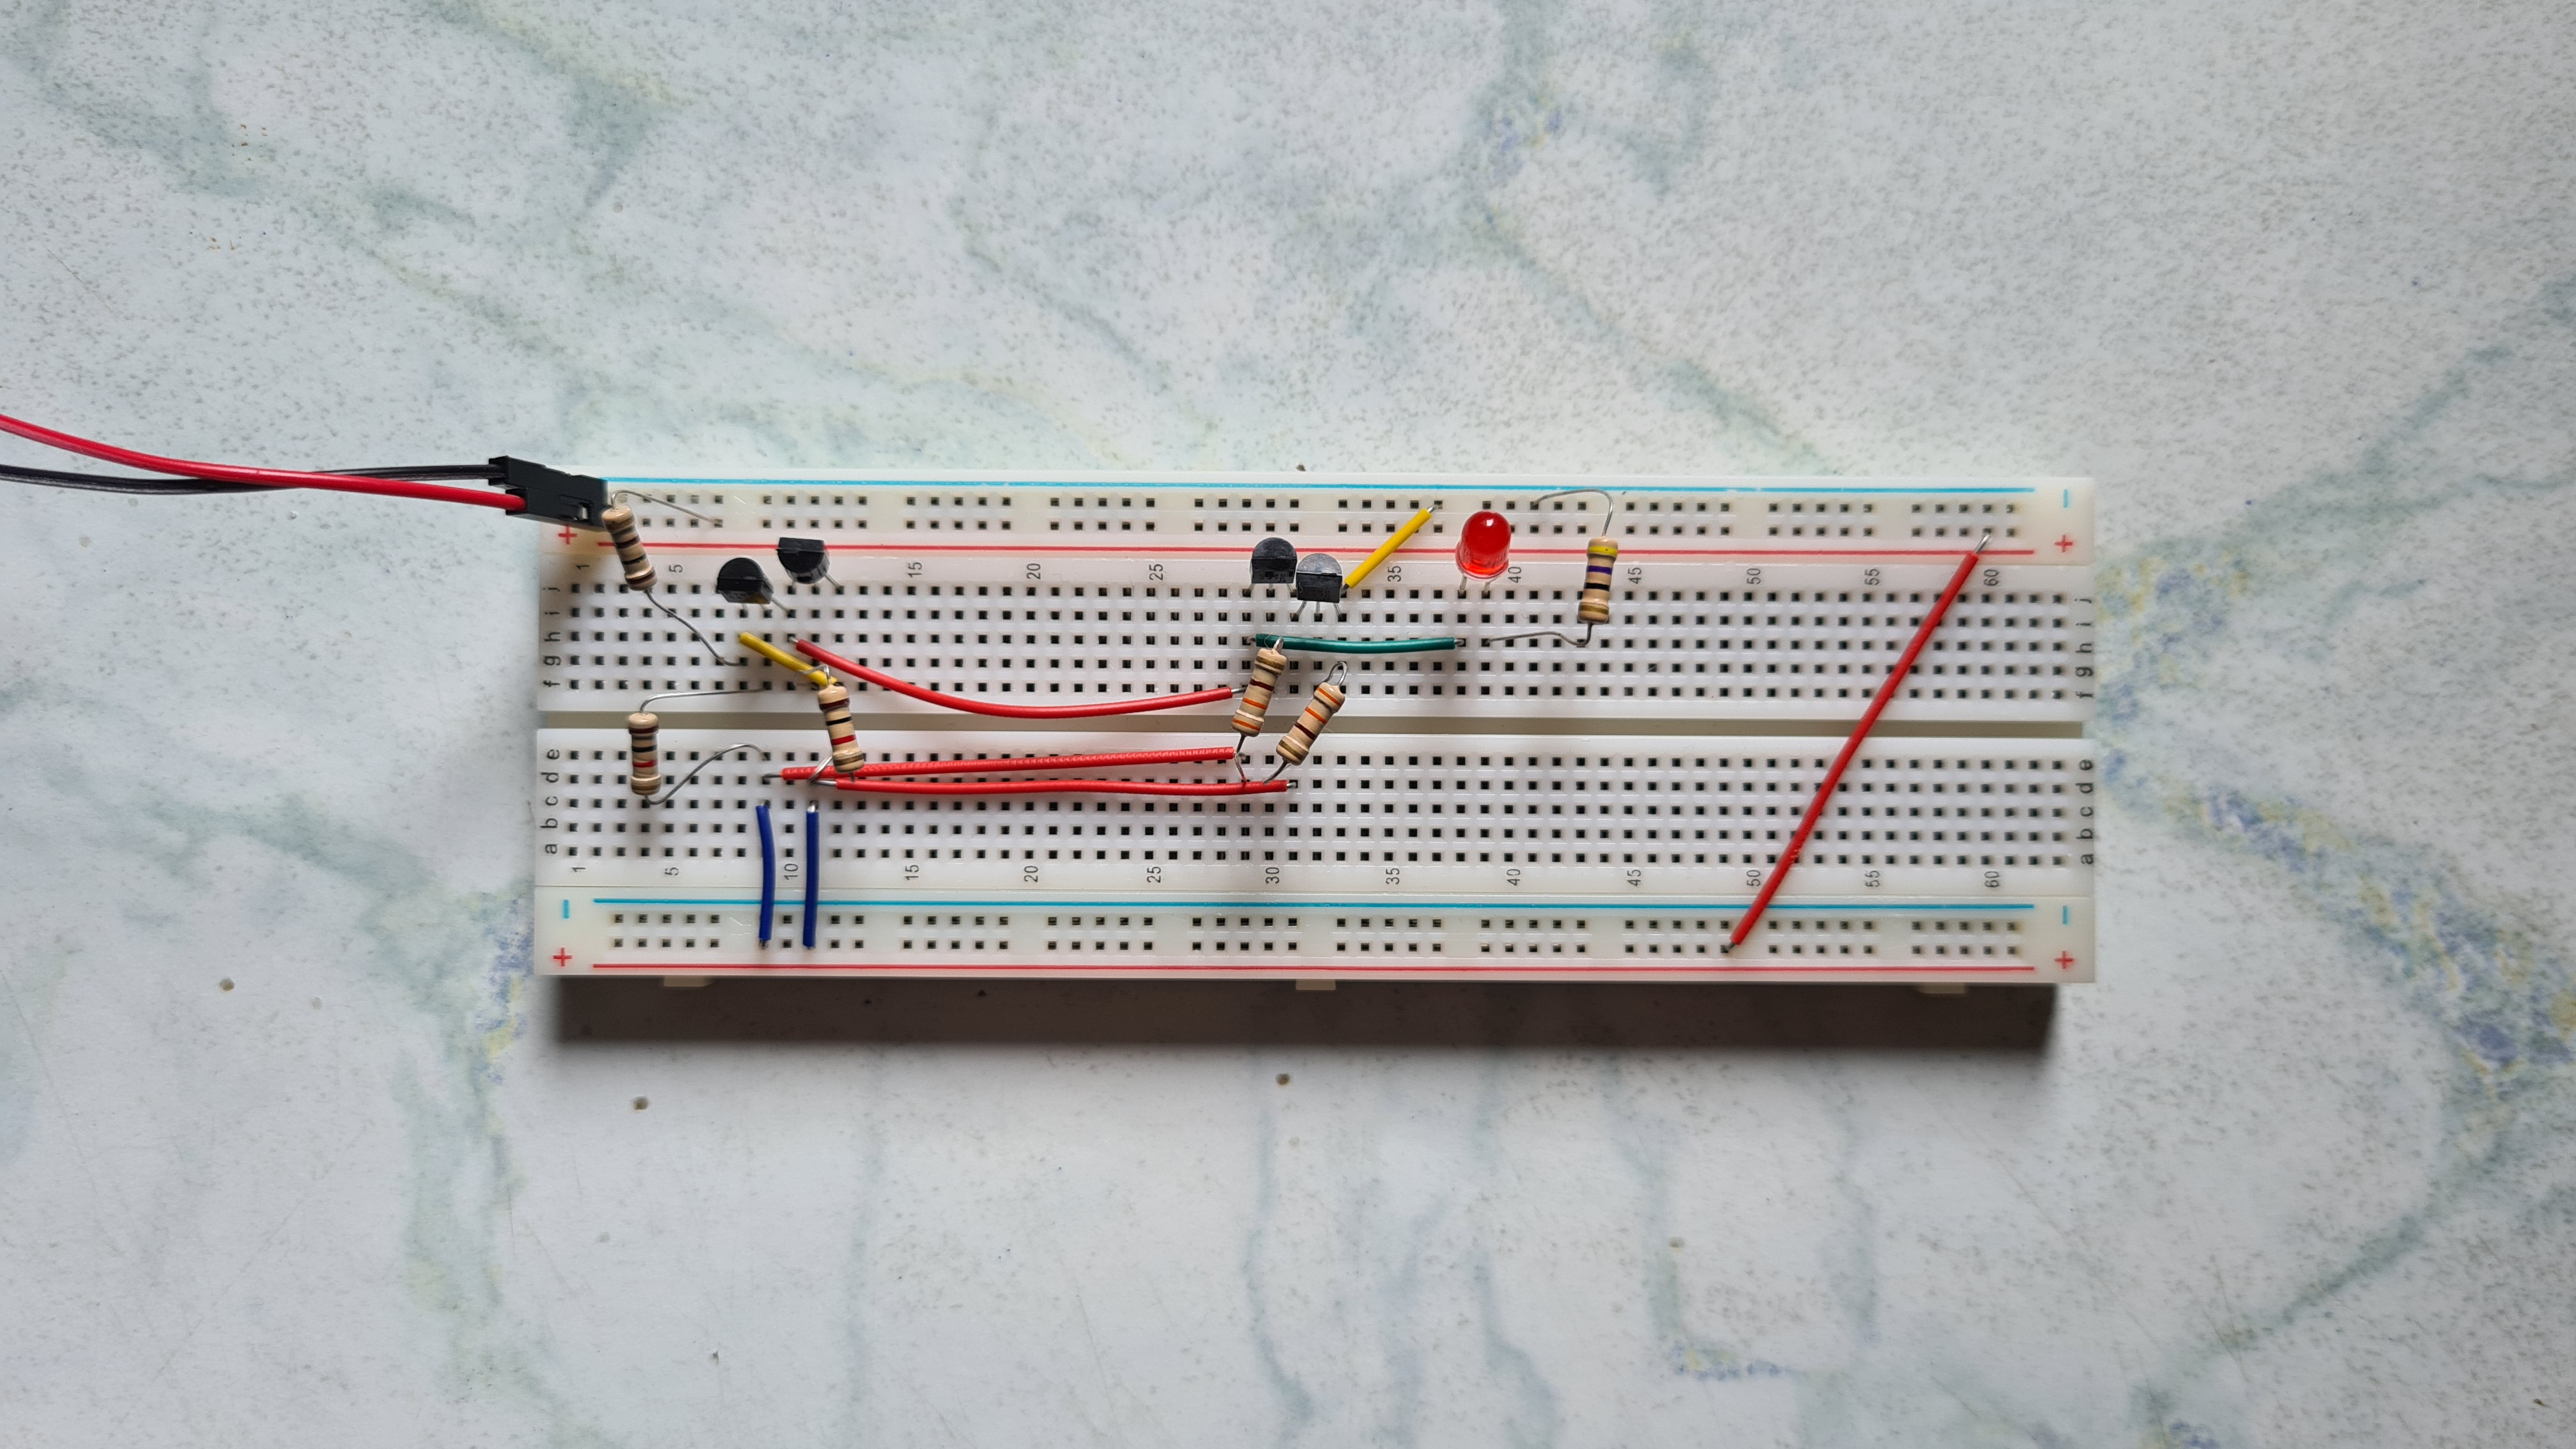
\includegraphics[height=4cm, keepaspectratio]{./Fotos/EXOR-11.jpg}
	\end{minipage}
	\caption{Praktischer Aufbau des EXOR-Gatters in allen möglichen Zuständen.}
\end{figure}\\
\newpage

\subsection{Halbaddierer}
Der schematische Aufbau des Halbaddierers ist in \cite{zimmermann1998binary} abgebildet. Dieses logische Bauteil besitzt zwei Ausgänge. Deshalb wird die Wahrheitstabelle um eine weitere Spalte ergänzt. Die beiden Ausgänge können mit \gqq{$s$} und \gqq{$c_{out}$} (\gqq{carry out}) beschriftet werden. \gqq{$s$} stellt hierbei die Summe der Addition dar. \gqq{$c_{out}$} gibt an, ob sich bei der Rechenoperation ein Überlauf ereignet.\\
\begin{figure}[h]
	\centering
	\hspace{1cm}
	\begin{tabular}{|c|c|c|c|}
		\hline
		\textbf{A} & \textbf{B} & \textbf{$s$} & \textbf{$c_{out}$} \\
		\hline
		0 & 0 & 0 & 0 \\
		1 & 0 & 1 & 0 \\
		0 & 1 & 1 & 0 \\
		1 & 1 & 0 & 1 \\
		\hline
	\end{tabular}
	\caption{Wahrheitstabelle für den Halbaddierer}
\end{figure}\\
Sind A und B auf LOW, so ist $s$ ebenso auf LOW ($0+0=0$). Ist entweder A oder B auf HIGH, so liegt $s$ gleichermaßen auf HIGH ($1+0=1$ bzw. $0+1=1$). Sind A und B auf HIGH, so ereignet sich ein Überlauf ($1+1=10$). $s$ liegt hierbei auf LOW. Allein in diesem Fall liegt $c_{out}$ auf HIGH.\\\\
Die Umsetzung dieses Bauteils erfolgt durch die Verwendung zweier Logikgatter. Das Verhalten von $s$ ist identisch mit dem des EXOR-Gatters. $c_{out}$ verhält sich übereinstimmend zum UND-Gatter. Wie in \fancyref{EXOR} erwähnt, werden größere Logikschaltungen aus npn-Transistoren instabil. Daher wird zukünftig überwiegend auf vorgefertigte Logikgatter zurückgegriffen.\\
\newpage
\begin{figure}[h!]
	\centering
	\begin{circuitikz}
		
		% EXOR IC
		
		\draw[black, thick] (-1, 2) -- (2, 2) -- (2, -2) -- (-1, -2) -- cycle;
		\draw[black, thick] (.25, 2) .. controls (.25, 1.5) and (.75, 1.5) .. (.75, 2);
		
		
		\draw (-1, 1.5) node[right]{$A_1$};
		\draw (-1, 1) node[right]{$B_1$};
		\draw (-1, .5) node[right]{$Y_1$};
		
		\draw (-1, 0) node[right]{$A_2$};
		\draw (-1, -.5) node[right]{$B_2$};
		\draw (-1, -1) node[right]{$Y_2$};
		
		\draw (-1, -1.5) node[right]{$\text{GND}$};
		
		
		\draw (2, 1.5) node[left]{$\text{VCC}$};
		\draw (2, 1) node[left]{$B_4$};
		\draw (2, .5) node[left]{$A_4$};
		
		\draw (2, 0) node[left]{$Y_4$};
		\draw (2, -.5) node[left]{$B_3$};
		\draw (2, -1) node[left]{$A_3$};
		
		\draw (2, -1.5) node[left]{$Y_3$};
		
		\draw[gray] (.5, -2) node[below]{EXOR};
		
		% END EXOR IC
		
		\draw (-1, -1.5) to[short] (-1.5, -1.5) to[short] (-1.5, -3) node[ground]{};
		\draw (2, 1.5) to[short] (2.5, 1.5) to[short, -o] (2.5, 3) node[above]{$VCC$};
		
		\draw (-9, 0) node[left]{A} to[short, o-] (-4.5, 0) to[short] (-4.5, 1.5) to[short] (-1, 1.5);
		\draw (-9, -1) node[left]{B} to[short, o-] (-4, -1) to[short] (-4, 1) to[short] (-1, 1);
		
		\draw (-1, .5) to[short] (-3, .5) to[short] (-3, -5) to[short, -o] (5, -5) node[right]{$s$};
		
		\draw (-4, -5) node[npn](T1){$T_1$};
		\draw (-4, -7) node[npn](T2){$T_2$};
		
		\draw (T1.E) to[short] (T2.C);
		\draw (T1.C) to[short, -o] ++(0, 2) node[above]{$VCC$};
		
		\draw (T1.B) to[R, l=$R_1$, a=\SI{1}{k\ohm}] (-6.5, -5) to[short, -*] (-6.5, 0);
		\draw (T2.B) to[R, l=$R_2$, a=\SI{1}{k\ohm}] (-6.5, -7) to[short] (-7, -7) to[short, -*] (-7, -1);
		
		\draw (T2.E) to[short] (-4, -8) to[short, -o] (5, -8) node[right]{$c_{out}$};
		\draw (-4, -8) to[R, l=$R_3$, a=\SI{1}{k\ohm}, *-] (-4, -10) node[ground]{};
		
		
		\draw[gray, very thick, densely dashed] (-8, 4) -- (4, 4) -- (4, -11) -- (-8, -11) -- cycle;
		\draw (4, -11) node[above right, gray]{Halbaddierer};
		
	\end{circuitikz}
	\caption{Schaltplan für den Halbaddierer, bestehend aus jeweils einem EXOR- und UND-Gatter.}
\end{figure}

